% Centro de Estadística y Matemática Aplicada
% Universidad Simón Bolívar
% Plantilla LaTeX para manuscritos (tesis y pasantías)
% pregrado y postgrado
%
% Andrés M. Sajo-Castelli
% Carlos Contreras
%
% 15 Abril 2015 -- primera versión pública
% ...
% 11 Mayo 2018 --- Se agrega bibliografía en castellano via babelbib
%
\documentclass[pregrado]{tesis-usb}

% paquetes
\usepackage[utf8]{inputenc}
\usepackage{verbatim, acronym, amsmath, amsfonts, amssymb, float, pdfpages}
% \usepackage{hyperref}

% estilo de las referencias
\usepackage[fixlanguage]{babelbib-and}\selectbiblanguage{spanish}
\usepackage{url}
\bibliographystyle{babplain-lf}

\usepackage{graphicx}
\graphicspath{ {../imgs/} }

\usepackage{bookmark}

\autor{Ricardo Münch}
\autori{R. Münch}
\usbid{11-10684}
\titulo{Desarrollo de la versión 2 de la aplicación web eFuel}
\fecha{Septiembre~de~2018}
\agno{2018}
\fechadefensa{15~de~noviembre~de~2018}
\tutor{Tutor Académico: Prof. Soraya Carrasquel}
\usarcotutor
\cotutor{Tutor Industrial: Ing. José Cerqueiro}
\trabajo{Informe de Pasantía}
\coord{Ingeniería de la Computación}
\grado{Ingeniero en Computación}
\carrera{Ingeniería de la Computación}
\programa{Nombre del Programa}
\juradouno{Nombre y Apellido}
\juradodos{Nombre y Apellido}
\juradotres{Nombre y Apellido}

% Cambia comillas simple por comilla cerrada en ambiente verbatim
\makeatletter
\let \@sverbatim \@verbatim
\def \@verbatim {\@sverbatim \verbatimplus}
{\catcode`'=13 \gdef \verbatimplus{\catcode`'=13 \chardef '=13 }}
\makeatother

\begin{document}

    \frontmatter
    \maketitle
    \begin{resumen}
        El presente documento tiene por objetivo describir el proceso de desarrollo de la aplicación web eFuel durante el período Abril-Septiembre 2018 en la empresa iKêls Consulting, una empresa que se especializa en el desarrollo de aplicaciones y sitios web para el sector corporativo utilizando Umbraco como la plataforma principal de manejo de contenido (CMS). La aplicación desarrollada permite a las estaciones de servicio de combustible la colocación de sus pedidos al mayorista. Una primera versión de esta aplicación fue desarrollada hace más de 10 años utilizando tecnología obsoleta, por lo tanto, la empresa requiere de un proceso re-ingeniería completo para adaptar la solución a plataformas y modelos de gestión más modernos así como integrarla como un módulo o paquete del CMS Umbraco. El desarrollo se dividió en varias fases: inducción del pasante, análisis de requerimientos, diseño, implementación y documentación, la metodología para llevar a cabo estas fases se basa en las ideas de Scrum. En cuanto a las tecnologías utilizadas, la aplicación fue desarrollada sobre la plataforma Umbraco CMS que está, a su vez, construida sobre la plataforma ASP.NET de Microsoft, los lenguajes de programación utilizados fueron C\# para el back end y HTML, CSS y JavaScript para el front end, para la base de datos se usó el DBMS SQL Server de Microsoft. Como resultado del proyecto de pasantía se obtuvo una versión funcional de la solución y se cumplieron los objetivos planteados.
    \end{resumen}
    \tableofcontents
    \listoffigures

    \mainmatter
    \chapter*{Introducción}

Este proyecto fue realizado en el marco de los Cursos de Cooperación Técnica y Desarrollo Social de la Universidad Simón Bolívar, consistió en el desarrollo de una aplicación web llamada \emph{eFuel} que sirve como apoyo al sistema de gestión de recursos de una empresa mayorista de combustibles. La aplicación desarrollada permite a los usuarios realizar pedidos de combustible y monitorear el estado de dichos pedidos, de pagos y de facturas. Además, permite gestionar entidades del modelo de negocio como clientes, transportes y productos.

El proyecto se llevó a cabo en la empresa iKêls Consulting \cite{ikelsAbout}, la cual se especializa en el desarrollo de aplicaciones y sitios web para el sector corporativo utilizando Umbraco como la plataforma principal de manejo de  contenido. Umbraco \cite{umbraco} es una herramienta de código abierto desarrollada en Dinamarca usando el lenguaje C\# y ASP.NET para sistemas Windows de Microsoft que cuenta con una gran aceptación a nivel mundial y una amplia comunidad de desarrolladores.

\section*{Antecedentes}
Entre los activos de la empresa se encuentra una aplicación web (\emph{eFuel}) que permite a las estaciones de servicio de combustible la colocación de sus pedidos al mayorista. Dicha aplicación fue desarrollada hace más de 10 años usando tecnología Classic ASP. Classic ASP es un motor de scripting para servidores cuya última versión fue desarrollada en el año 2000, y que fue reemplazado por ASP.NET en el año 2002. No se sabe de otra aplicación web que ofrezca este servicio.

La primera versión de eFuel desarrollada no se encuentra en un estado funcional. Tampoco se pudo emular porque no se pudo replicar el ambiente original de la aplicación. Esta primera versión estaba conformada por 4 módulos de funcionalidad:

\begin{itemize}
    \item \emph{Seguridad}: controlaba el acceso a la aplicación y sus datos.
    \item \emph{Pedidos}: inserción de pedidos de combustible.
    \item \emph{Pagos}: operaba como auxiliar contable del sistema de facturación interno de la organización (mayorista). 
    \item \emph{Datos}: ofrecía la posibilidad de activar y desactivar registros correspondientes a clientes, productos y otros parámetros no disponibles en el \ac{ERP} de la organización. Adicionalmente poseía una bitácora que registraba las operaciones realizadas en el sistema.
\end{itemize}

\section*{Planteamiento del problema}
Las empresas de distribución de combustible deben atender diariamente un volumen importante de pedidos a lo largo del territorio nacional. Este proceso involucra a múltiples actores, tiene un alto impacto en la sociedad y su coordinación es una labor tediosa y delicada que requiere personal especializado. Se requiere reducir los errores humanos, mejorar la eficiencia, aumentar la calidad de la información asociada al proceso.

Con los procesos manuales tradicionales, el proceso de pedidos de combustible consume mucho tiempo y esfuerzo, está sujeto a muchos errores debido a las múltiples variables involucradas y no tiene flexibilidad para responder con rapidez a los cambios propios de la demanda de las \ac{EE/SS}.

\section*{Justificación e importancia}
Debido al alto impacto que tiene en la dinámica diaria de las personas y negocios, la inversión en herramientas de apoyo producirá mejoras inmediatas en todos los aspectos del proceso. Al automatizar las tareas de pedido de combustible y asignación de pagos, se reduce considerablemente la cantidad de errores humanos que se cometen con los métodos manuales. Por otro lado, se consolida toda la información de pedidos y pagos (pendientes y realizados) de todas las estaciones de servicio en un solo sitio de acceso fácil y seguro.

\section*{Objetivo general}
Desarrollar una nueva versión de la aplicación web eFuel integrada con el \ac{CMS} Umbraco \cite{umbraco} para el ingreso y administración de pedidos de combustible (cisternas).

\section*{Objetivos específicos}
\begin{itemize}
    \item Crear el módulo de administración de clientes, productos, precios, vehículos, rutas y conductores. Las funcionalidades de este módulo incluyen:
    \begin{itemize}
        \item Crear, editar y eliminar registros.
        \item Calcular costo de cisterna según volumen y precios de productos.
        \item Asignar vehículos y tipos de producto a clientes.
        \item Listar registros con mecanismo de búsqueda.
    \end{itemize}

    \item Crear el módulo de administración de pedidos. Las funcionalidades de este módulo incluyen:
    \begin{itemize}
        \item Crear, editar y eliminar pedidos mediante consola especializada.
        \item Diferenciar opciones según perfil del usuario.
        \item Listar y filtrar pedidos con opción de exportar en un archivo.
    \end{itemize}

    \item Crear el módulo de conciliación de pagos. Este módulo cuenta con las siguiente funcionalidad:
    \begin{itemize}
        \item Mecanismo para registro de pagos totales o parciales.
        \item Mecanismo de conciliación y asignación de pagos a pedidos.
    \end{itemize}

    \item Crear el módulo de registro de usuarios y perfiles. A través de este módulo los usuarios pueden:
    \begin{itemize}
        \item Registrar y editar usuarios con perfil de permisos.
        \item Asociar usuarios a clientes.
    \end{itemize}
\end{itemize}
    \chapter{Entorno empresarial}
En este capítulo se describe a la empresa en la cual se desarrolló el proyecto de pasantía. Comprende una breve reseña histórica, su misión y visión, la estructura organizacional y el área a la cual el pasante estuvo asignado.

\section{Antecedentes de la empresa}
IKêls Consulting se creó el año 2008 como una empresa dedicada al desarrollo de soluciones en el área de Sistemas de Información. Los fundadores contaban con una amplia trayectoria en los procesos y tecnología para la elaboración de documentación técnica avanzada (por ejemplo normas ISO para construcción de plantas petroquímicas).

Para aprovechar la experiencia previa los productos y servicios se concentran en el área de aplicaciones web (por ejemplo, sistemas de manejo de contenido o CMS) para el sector corporativo atendiendo a un selecto grupo de clientes con presencia local e internacional.

Actualmente, las actividades principales se concentran en:

\begin{itemize}
  \item Construcción de portales web en múltiples idiomas y que pueden ser administrados por sus propios dueños. Esto incluye la programación de módulos especiales para integrar información desde y hacia sistemas externos, desplegar datos de manera amigable o generar notificaciones automáticas dependientes de actividades de los visitantes u otros eventos.
  \item Apoyo en la gestión de contenido de portales web.
  \item Consultoría y gestión para optimizar las variables asociadas al rendimiento y desempeño de las páginas web. Teniendo especial interés en el monitoreo de presencia en buscadores, evaluación del perfil de los visitantes y garantizar un nivel adecuado de usabilidad en diferentes dispositivos, etc.
  \item Desarrollo de productos personalizados que complementen las ventajas y facilidades de los dispositivos móviles en sincronización con mecanismos de soporte en servidores web.
  \item Desarrollo de soluciones especializadas para ofrecer bajo el modelo SaaS o Software as a Service.
\end{itemize}

\section{Misión}
Proveer productos y servicios en el área de sistemas de información que permitan una comunicación efectiva de nuestros clientes con su público y también sirva como plataforma de trabajo donde se aprovechen las innovaciones y ventajas de las tecnologías más modernas.

\section{Visión}
Deseamos ser un proveedor confiable, que ofrece un alto valor agregado en cada producto o servicio que prestamos a nuestros clientes.

\section{Ubicación del pasante}
El proyecto de pasantía pertenece al grupo de desarrollo de aplicaciones y cuenta con la dirección del Presidente de la Empresa y con el apoyo de los ingenieros líderes del grupo.
    \chapter{Marco Teórico}
En el presente capítulo se definen las bases teóricas sobre las cuáles se apoya el proyecto.

\section{Bases Teóricas}

\subsection{CMS}
Un CMS, por sus siglas en inglés \textit{Content Management System} (Sistema de Gestión de Contenidos), es una aplicación de software que provee algún nivel de automatización a las tareas de manejo de contenido. Un CMS permite a los usuarios crear nuevo contenido, editar contenido existente, y hacer el contenido accesible al público. \cite{cmsBarker}

Desde el punto de vista de un editor un CMS consta, básicamente, de 2 partes: una interfaz para la edición de contenido (referido como el \textit{back-end}, esto es, la capa de acceso a los datos de la aplicación) y una interfaz para mostrar el contenido publicado (referido como el \textit{front-end}, es decir, la capa de presentación de la aplicación).

El uso de un CMS facilita las tareas de mantenimiento y de generación de contenido, especialmente para usuarios que no tienen preparación técnica especial. Los usuarios de la aplicación eFuel serán, en su mayoría, personal sin conocimientos especializados en el área de computación, esta es una de las razones por las cuales resulta conveniente desarrollar el sistema sobre un CMS.

Además, el CMS sobre el cual se desarrolló la aplicación posee funcionalidades ya implementadas que son necesarias para el sistema: la autenticación de usuarios, permisología, interfaces para realizar operaciones sobre la base de datos, entre otras. La plataforma también cuenta con una variedad de librerías y de módulos que facilitan el desarrollo del sistema. También cabe destacar que la empresa tiene varios años de experiencia desarrollando aplicaciones web con un CMS lo cual facilitó el desarrollo del sistema.

\subsection{Modelo Cliente-Servidor}
Arquitectura de redes de computadoras que divide el trabajo entre 2 entidades: un cliente y un servidor. El cliente le envía una solicitud al servidor y espera una respuesta. Por otra parte, el servidor recibe la solicitud, lleva a cabo el trabajo requerido y devuelve una respuesta al cliente. \cite{redesTanenbaum} El servidor mantiene una relación de uno-a-muchos con los clientes. Es importante destacar que los términos “cliente” y “servidor” pueden referirse tanto a máquinas como a programas o procesos. Esta arquitectura es ampliamente utilizada en aplicaciones web.

\subsection{MVC}
MVC, siglas para Modelo-Vista-Controlador, es un modelo de diseño de aplicaciones compuesto por 3 partes: el Modelo (datos), la Vista (presentación de los datos e interfaz con el usuario) y el Controlador (proceso que maneja la entrada de los usuarios y el acceso a los datos). \cite{mvcKrasner} Al separar la aplicación en estos 3 componentes se reduce la complejidad del diseño arquitectónico y se incrementa la reusabilidad, flexibilidad y mantenimiento del código. Adicionalmente, se pueden realizar cambios sobre un componente sin afectar a los demás, lo cual permite que cada componente tenga ciclos de desarrollo independientes.

Actualmente, este patrón es ampliamente utilizado en el desarrollo de aplicaciones web ya que resulta muy natural acoplarlo con el modelo cliente-servidor que utiliza la web. El sistema eFuel fue desarrollado sobre una plataforma de desarrollo web que implementa el patrón MVC y, en consecuencia, el código tiene la estructura descrita por este patrón.

\subsection{API}
Un API, siglas en inglés para \textit{Application Programming Interface}, es un conjunto de comandos, funciones, protocolos y objetos que exponen los datos de una aplicación de software, es decir, establecen las reglas y los mecanismos a través de los cuales se puede tener acceso a ellos. \cite{apiChristensson}

Normalmente, aplicaciones externas disponen del API de una aplicación para obtener datos de esta última y usarlos para proveer algún servicio a sus usuarios.

\subsection{Servicio Web}
Un servicio web es un sistema de software diseñado para soportar interacción máquina-máquina a través de una red, proveen una vía estándar para la interoperabilidad entre distintas aplicaciones de software ejecutadas en distintas plataformas y ambientes. \cite{webServiceW3C} Típicamente, los sistemas externos tienen acceso al servicio web a través de un API.

El proyecto presente incluye el desarrollo de un módulo de servicios web para el acceso a algunos datos de la aplicación, por ejemplo, datos para generar tablas informativas.

\subsection{REST}
Transferencia de Estado Representacional o REST, por sus siglas en inglés, es un estilo de arquitectura para sistemas de hipermedia distribuidos (como la \textit{World Wide Web} o red informática mundial) que define una serie de restricciones que, cuando se aplican en conjunto, enfatizan la escalabilidad de interacciones entre componentes, la generalidad de las interfaces y el despliegue independiente de componentes. \cite{restFielding}

Las restricciones definidas para los sistemas REST son las siguientes:

\paragraph{Separación Cliente-Servidor} .
\paragraph{Sin estado (\emph{stateless} en inglés)} .
\paragraph{Permite el uso de memoria caché} .
\paragraph{Interfaz uniforme} cada solicitud al servidor debe tener los mismos componentes .
\paragraph{Sistema por capas} .

Se dice que un servicio web o el API de un servicio web es \textit{RESTful} cuando cumple con estas restricciones.
    \chapter{Marco Tecnológico}
En este capítulo se definen las tecnologías y herramientas utilizadas para el desarrollo del sistema. Entre estas se incluyen los \textit{frameworks} utilizados para el desarrollo (ASP.NET, ASP.NET MVC, ASP.NET Web API y Umbraco), los lenguajes utilizados (C\# para el \textit{backend}, y HTML, CSS y JavaScript para el \textit{frontend}, como es común en el desarrollo web), la herramienta de control deversiones (Git) y el entorno de desarrollo (Visual Studio).

\section{Frameworks}
    \subsection{ASP.NET}
    ASP.NET es un modelo de desarrollo Web unificado que incluye los servicios necesarios para construir aplicaciones Web empresariales con un mínimo de codificación. ASP.NET es parte de .NET Framework y al codificar las aplicaciones en ASP.NET se tiene acceso a las clases de .NET Framework. \cite{asp.netMicrosoft}

    \subsection{ASP.NET MVC}
    ASP.NET MVC es un marco de trabajo (o \textit{framework} en inglés) para construir aplicaciones web escalables, basadas en estándares y usando patrones de diseño bien establecidos (el patrón MVC) y el poder de ASP.NET y .NET Framework. \cite{asp.netMVCMicrosoft}

    Se utilizó este marco de trabajo para el desarrollo del módulo \textbf{EF\_Core} (ver sección \emph{sección de arquitectura}) del proyecto, allí están implementados los controladores (ver sección \ref{mvc}) de la aplicación web.

    \subsection{ASP.NET Web Api}
    ASP.NET Web API es un marco de trabajo que facilita la construcción de servicios HTTP que llegan a una amplia gama de clientes, incluyendo navegadores y dispositivos móbiles. ASP.NET Web API es una plataforma ideal para construir aplicaciones RESTful en .NET Framework. \cite{asp.netWebAPIMicrosoft}

    Este marco de trabajo se utilizó para el desarrollo del módulo \textbf{EF\_API} (ver sección \emph{sección de arquitectura}) del proyecto, allí están implementados los servicios del API para acceder a información del sistema (ver sección \ref{webService}) de la aplicación web.

    \subsection{Umbraco}
    Umbraco es un Sistema de Gestión de Contenido gratuito y de código abierto construido sobre ASP.NET, fue desarrollado en Dinamarca y su primera versión fue lanzada en el año 2005. Umbraco cuenta con funcionalidades que son necesarias para el sistema: la autenticación de usuarios, permisología, interfaces para realizar operaciones sobre la base de datos, entre otras. La plataforma también cuenta con un repositorio de paquetes y extensiones que proveen otras funcionalidades útiles para la aplicación web y provee una variedad de librerías y de módulos que facilitan el desarrollo del sistema.

    Cabe destacar que la empresa tiene varios años de experiencia desarrollando aplicaciones web con Umbraco y varios de sus empleados tienen certificaciones y un nivel alto de conocimiento de la plataforma lo cual facilitó el desarrollo del sistema. La aplicación web eFuel fue desarrollada con Umbraco v7.10.

    \subsection{Bootstrap}


\section{Lenguajes}
A continuación se definen brevemente los lenguajes de programación utilizados para el desarrollo del proyecto divididos en \textit{front-end} y \textit{back-end}.

\subsection{\emph{Front-end}}
\subsubsection{HTML}
HTML (siglas en inglés para Lenguaje de Marcado de HiperTexto), es el lenguaje de marcado central de la \textit{World Wide Web} (red informática mundial). Originalmente, HTML fue diseñado principalmente para describir semánticamente documentos científicos. Sin embargo, la generalidad de su diseño ha permitido que sea adaptado, en los años siguientes, para describir otros tipos de documentos y hasta aplicaciones. \cite{htmlW3C}

Es el lenguaje que se usa para definir la estructura y el contenido de una página web, en el caso de este proyecto se usa para describir las vistas del sistema.

\subsubsection{CSS}
Hojas de Estilo en Cascada, o CSS por sus siglas en inglés (\textit{Cascading Style Sheets}), es un lenguaje de hojas de estilo que permite a los autores y usuarios adjuntar estilos (\textit{e.g.} fuentes y espaciados) a documentos estructurados (\textit{e.g.} documentos de HTML). Al separar el estilo de presentación del contenido de los documentos, se simplifica la autoría y el mantenimiento de los sitios. \cite{cssW3C}

\subsubsection{JavaScript}
JavaScript es un lenguaje de \textit{scripting} o programación que permite la creación de contenido dinámico, control de multimedia, animación de imágenes \cite{jsMozilla}. \emph{mencionar las llamadas al servidor para traer datos con el API}


\subsection{\emph{Back-end}}
\subsubsection{C\#}
C\# es un lenguaje con seguridad de tipos y orientado a objetos que permite a desarrolladores construir una variedad de aplicaciones robustas y seguras que corren sobre .NET Framework. \cite{cSharpMicrosoft}

\section{Control de versiones}
\subsection{Git}
Git es un sistema de gestión de versiones rápido, escalable y distribuido con un rico conjunto de comandos que proveen operaciones de alto nivel y acceso completo a internos. \cite{gitGit} Fue desarrollado por Linus Torvald en el año 2005 para facilitar el trabajo de varios desarrolladores sobre un mismo proyecto. Permite llevar el seguimiento de los cambios a un grupo de archivos y sincronizar varios repositorios en máquinas distintas.

Este es el sistema de gestión de versiones usado en la empresa en la que se desarrolló el proyecto.

\section{Entorno de trabajo}
\subsection{Visual Studio}
Visual Studio es un ambiente de desarrollo integrado que permite editar, depurar, compilar y publicar código. \cite{visualStudioMicrosoft} Este ambiente de desarrollo incluye una gran cantidad de funcionalidades para facilitar el desarrollo de software: depuración del código paso a paso y con información detallada de las variable y otras entidades del programa, instrucciones de compilación complejas para la aplicación, descarga y actualización paquetes y librerías, integración con Git, \textit{IntelliSense} de Microsoft para la completación de partes de código usando el contexto de la aplicación (clases y sus relaciones y métodos), entre otras.

Este entorno de trabajo está muy bien integrado con los \textit{frameworks} utilizados para el proyecto (ASP.NET y sus extensiones/derivados), por lo que su uso resultó ventajoso y natural para el desarrollo del proyecto.

\subsection{Trello}
Trello es una herramienta de colaboración que organiza las tareas de un proyecto en tablas. Trello informa en qué se está trabajando, quién está trabajando en qué, y el estado de una tarea en el proceso de desarrollo.

Cada tabla tiene varias listas y cada lista contiene tarjetas. Una tabla corresponde a un proyecto, una lista corresponde al estado de una tarea y una tarjeta a una tarea, por ejemplo, en una tabla suele haber 3 listas: \emph{Por hacer}, \emph{Haciendo} y \emph{Lista}. Las tarjetas contienen una descripción de la tarea, la o las personas asignadas y puede tener una fecha límite de entrega. A medida que se va completando trabajo se van moviendo las tarjetas de una lista a otra.

Resultó una herramienta útil para llevar el control de las tareas realizadas y por realizar. Se usó esta herramienta como apoyo para el uso de Scrum (ver capítulo \ref{marcoMetodologico}).
    \chapter{Marco Metodológico}

    \chapter{Desarrollo} \label{development}
En este capítulo se describe la aplicación web eFuel con sus módulos y funcionalidades, luego se narra cómo fue el desarrollo del proyecto. El desarrollo se divide en 3 fases: una fase de inducción donde el pasante se familiarizó con las herramientas y tecnologías necesarias para realizar el proyecto, una fase de desarrollo que consta de 6 Iteraciones de Scrum y una última fase de documentación.

A continuación la descripción de la aplicación seguido de las fases del desarrollo de la misma durante el proyecto de pasantía.

\section{La aplicación web eFuel}
Para este proyecto se desea desarrollar una nueva versión de la aplicación web eFuel basada en tecnologías modernas como ASP.NET y Umbraco. No se usó código de la primera versión, se partió desde cero a programar la nueva versión. Se usaron documentos de la versión original para guiar el desarrollo de la nueva versión de eFuel, especialmente en el diseño de las entidades de la base datos y en las funcionalidades generales (módulos) del sistema.

\subsection{Nueva versión de eFuel}
La nueva versión de eFuel desarrollada para este proyecto es una aplicación web que permite a las estaciones de servicio de combustible la colocación de sus pedidos al mayorista. La aplicación permite consultar información del estado de los pedidos (si fueron despachados y si fueron pagados), asociar facturas a pedidos y asociar pagos a facturas, también permite consultar información sobre otras entidades del dominio de negocio como clientes (estaciones de servicio), transportes disponibles según la zona del cliente, productos disponibles y sus precios. Además, permite importar y exportar información para intercambiar con el \ac{ERP} del mayorista y, de esta manera, servir como sistema de apoyo para este.

\subsubsection{Módulos de funcionalidad}
El sistema se descompone en 4 módulos de funcionalidad: Pedidos, Pagos, Administración y Seguridad. A continuación una breve descripción de las funcionalidades de cada módulo:

\begin{itemize}
    \item \emph{Pedidos}: módulo para la gestión de pedidos. Al crear un pedido se brinda la facilidad de seleccionar rápidamente la combinación de cliente-fecha-turno-transporte-productos. También permite mostrar un listado de los pedidos, filtrar la lista por cliente, transporte, rango de fecha o estado, y luego exportarla como un archivo de Excel. 
    \item \emph{Pagos}: módulo para la gestión de pagos y facturas. Con este módulo se pueden importar facturas desde un archivo de Excel generado por el \ac{ERP} del mayorista, éstas se asocian inmediatamente con un pedido. También se pueden gestionar los pagos, asociar pagos a facturas y exportarlos a un archivo de Excel.
    \item \emph{Administración}: módulo para la gestión de clientes, transportes, productos, zonas y turnos. Esto incluye creación, edición, consulta, listado, importación y eliminación de estas entidades del sistema.
    \item \emph{Seguridad}: este módulo controla el acceso a la aplicación para garantizar que únicamente las personas autorizadas puedan consultar los datos y realizar las operaciones que les corresponden. Se pueden crear y editar miebros, así como modificar los permisos de cada uno.
\end{itemize}

\subsubsection{Sobre los modelos de datos}
Las entidades del sistema las podemos dividir en 2 categorías: transaccionales y no transaccionales. Las entidades transaccionales son objetos que se van a generar con mucha frequencia durante el funcionamiento del sistema: pedidos, facturas y cobros; las no transaccionales no se generan con tanta frequencia: clientes, transportes, zonas, turnos y productos.

Al crear un nodo de contenido desde el back office de Umbraco se guarda cierta información adicional a las propiedades definidas por el programador: fechas de publicación, versiones, autor, entre otras. Esto no es conveniente para modelar las entidades transaccionales ya que se genera un volumen importante de éstas y mucha de esa información adicional no es necesaria. Por esta razón, se decidió modelar las entidades transaccionales como tablas en la base de datos independientes de las tablas de Umbraco las entidades no transaccionales se modelaron como Doctypes de Umbraco, que son definiciones de la estructura de un tipo de contenido (para más detalles ver la Sección \ref{conceptosUmbraco}).

En la Figura \ref{fig:esquema_general_nuevo} se muestra el esquema general del sistema.

\vspace{0.3cm}

\begin{figure}[ht]
    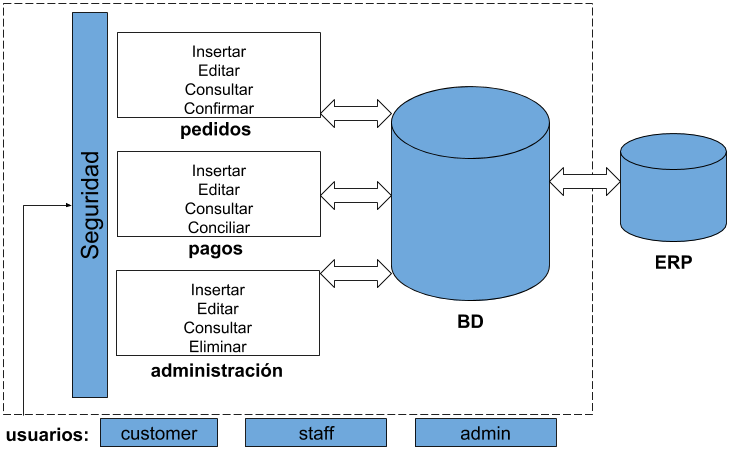
\includegraphics[width=\textwidth]{esquema_general_nuevo.png}
    \caption{Esquema general de los módulos de funcionalidad}
    \label{fig:esquema_general_nuevo}
    \centering
\end{figure}

Uno de los objetivos de la aplicación es servir como sistema de apoyo a los ERP de los mayoristas. Los sistemas ERP llevan el control de todas las entidades del negocio, entre estas están las estaciones de servicio, los transportes para los pedidos, los pedidos, las facturas, etc. La aplicación eFuel interactúa con el \ac{ERP} y le sirve de apoyo a éste manteniendo un registro separado de las entidades pertinentes a la inserción y el pago de pedidos de combustible. Esta interacción se da a través de importaciones y exportaciones de datos entre estos sistemas para que estén sincronizados.

\section{Fases del desarrollo}
\subsection{Fase de Inducción}
Esta fase tuvo una duración de 1 semana, el pasante realizó varios tutoriales y utilizó varios recursos (guías de Umbraco, videos de ASP.NET, entre otros) proporcionados por la empresa para inducir los conocimientos técnicos necesarios para llevar a cabo el proyecto. Las herramientas investigadas fueron: Umbraco, ASP.NET, SQL Server y Visual Studio.

\subsection{Fase de Desarrollo}
Esta fase duró 16 semanas continuas y se llevaron a cabo 6 Iteraciones donde se desarrolló la aplicación. A continuación una descripción del trabajo realizado en cada iteración.

\subsubsection{Análisis de requerimientos (1era Iteración)}
Se definió la arquitectura y la estructura de la base de datos. Además, se creó el repositorio de Git, el proyecto de Visual Studio y el sitio de Umbraco, y por otro lado, se eligió una plantilla de HTML para el \emph{look and feel} de la aplicación.

\vspace{0.3cm}
\textbf{Actividades realizadas:}
\begin{itemize}
    \item El pasante se familiarizó con la versión original de eFuel.
    \item El pasante se familiarizó con las reglas de negocio.
    \item El pasante junto con el dueño del producto definieron los actores del sistema, estos son: \emph{admin} (adminsitradores del sistema), \emph{staff} (empleados del mayorista) y \emph{customer} (empleados de las estaciones de servicio).
    \item Se listaron las funcionalidades básicas del front end a desarrollar. Esta lista de funcionalidades fue refinada y expandida a medida que se avanzo con el desarrollo. Listado de funcionalidades básicas elaborado:
        \begin{itemize}
            \item Listado de pedidos.
            \item Creación de pedidos.
            \item Listado de clientes, zonas y transportes.
            \item Listado de facturas.
        \end{itemize}
    \item Creación de la solución de Visual Studio con los módulos \texttt{EF\_Core}, \texttt{EF\_Core} y \texttt{EF\_\-Miscelaneous}.
    \item Creación del repositorio de Git y familiarización con las reglas del mismo.
    \item Se definieron las entidades de la base de datos del proyecto para poder implementar funcionalidades básicas del sistema. Esto incluyó decidir qué entidades se modelarán como tablas en la base datos directamente y qué entidades se modelarán como Doctypes de Umbraco. Finalmente se definieron las columnas que tienen las tablas de la base de datos.
    \item Se creó el sitio de Umbraco.
    \item Se evaluaron 2 plantillas de HTML para el estilo del sitio, ambas eran plantillas de tableros o \emph{dashboards}, se decidió utilizar una plantilla gratuita llamada Adminator, en la Figura \ref{fig:orderslist} se muestra una captura de la plantilla elegida.
\end{itemize}

\begin{figure}[H]
    \centering
    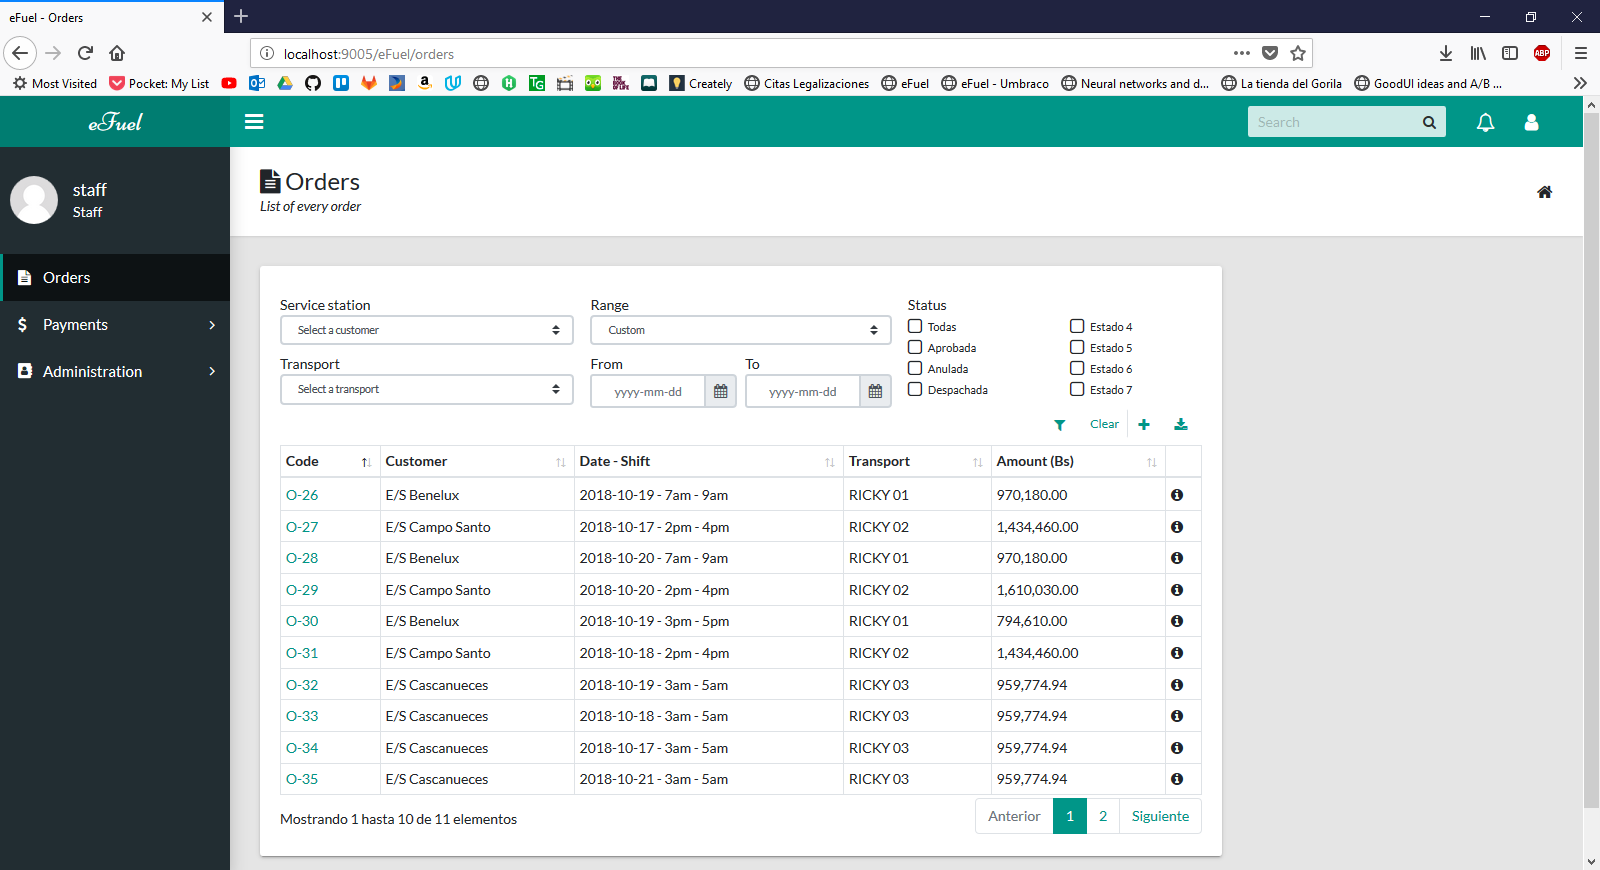
\includegraphics[width=0.7\textwidth]{./vistas/frontend/orders_list.png}
    \caption{Lista de pedidos (captura)}
    \label{fig:orderslist}
\end{figure}

\textbf{Duración:} 2 semanas.

\subsubsection{Módulo de Administración (2da Iteración)}
Se implementó la funcionalidad de manejo de las entidades principales de la aplicación: clientes, productos, transportes, zonas, turnos, pedidos, facturas y cobros. Para esto se implementó una interfaz en el back end de Umbraco usando Fluidity y se definieron los Doctypes y Data Types de las entidades a ser almacenadas como contenido de Umbraco.

También se empezó el desarrollo del front end de la aplicación. Al finalizar esta Iteración se tuvo una forma de manejar las entidades del sistema, ya sea a través del árbol de contenido de Umbraco o a través de la interfaz de Fluidity.

\vspace{0.3cm}
\textbf{Actividades realizadas:}
\begin{itemize}
    \item Se diseñaron los Doctypes y Data Types para las entidades no transaccionales (clientes, transportes, zonas, turnos y productos).
    \item Se desarrolló la interfaz de Fluidity para insertar registros en la base de datos de las entidades transaccionales. Esta actividad se realizó para tener una manera de gestionar las entidades transaccionales mientras no se tenga implementada esta funcionalidad en el front end.
    \item Se empezó el desarrollo de la barra de navegación, títulos de las páginas, menú de navegación para el front end. Éstos son elementos que tienen en común la mayoría de las vistas del front end.
    \item Se implementó la funcionalidad de listado de clientes en el front end. Primero se desarrolló el controlador para mostrar la vista y luego se diseñó la vista (el archivo de HTML). Se implementaron 2 controladores: uno de tipo \texttt{UmbracoApiController} para devolver los elementos de la lista y otro de tipo \texttt{SurfaceController} para devolver la vista como tal. También se desarrolló un script de JavaScript para manejar la organización de las tablas usando Datatables.
    \item Se implementó la funcionalidad de detalles de un cliente en el front end, se diseñaron el controlador y la vista correspondientes.
\end{itemize}

\textbf{Duración:} 3 semanas.

\subsubsection{Módulo de Administración (cont.) y Pedidos (3ra Iteración)}
Esta Iteración estuvo dedicada a terminar algunas funcionalidades del módulo de Administración en el front end y al desarrollo de la funcionalidad referente a los pedidos de combustible. Se desarrolló el listado de pedido con filtros, el formulario de creación de pedidos y la exportación de la lista de pedidos.

\pagebreak
\textbf{Actividades realizadas:}
\begin{itemize}
    \item Se implementaron las funcionalidades de listado de transportes y zonas en el front end. Para esto se diseñaron los controladores, las vistas y los scripts de JavaScript correspondientes.
    \item Se implementó la funcionalidad de listado de pedidos en el front end. Se diseñaron los controladores para devolver los datos de los pedidos y para devolver la vista, además se diseñó la vista de listado de pedidos y el script de JavaScript para manejar la tabla.
    \item Se implementó la funcionalidad de filtrado para la lista de pedidos en el front end. Para esto se modificó el archivo de JavaScript encargado de manejar la tabla para que también manejara los filtros aplicados a ésta y se agregaron varios métodos al controlador que devuelve la lista de pedidos. Cada método se encarga de seleccionar los pedidos de una lista de pedidos que tengan el mismo valor que el filtro deseado por el cliente en alguna propiedad. Hay un método por cada propiedad de los pedidos.
    \item Se implementó la funcionalidad de consultar los detalles de un pedido en el front end. Para esto se diseñaron el controlador y la vista correspondientes.
\end{itemize}

\textbf{Duración:} 2 semanas.

\subsubsection{Refactorización (4ta Iteración)} \label{refactorizacion}
Al realizar una revisión de la estructura del código se determinó que éste debía ser refactorizado para seguir el patrón MVC implementado por ASP.NET MVC, de esta manera el código se haría más fácil de mantener y extender al aprovechar las virtudes de este patrón.

Hasta ese punto del desarrollo los Controladores no reflejaban adecuadamente la estructura MVC y por lo tanto no se aprovechaba al máximo las virtudes de este patrón. Se habían implementado Controladores para cada "tipo" de funcionalidad, por ejemplo, en el caso de los pedidos había 3 Controladores: \texttt{OrdersController} que devolvía la lista de pedidos, \texttt{OrderDetailController} que devolvía la vista de detalles y \texttt{NewOrderFormContro\-ller} que devolvía el formulario para crear un nuevo pedido y procesaba la información de éste. Como se puede observar, esta estructura generó una elevada cantidad de archivos (uno por Controlador). El resultado fue código díficil de mantener (por la cantidad de archivos) y que no seguía las buenas prácticas sugeridas por el diseño de ASP.NET MVC.

Para resolver estos inconvenientes y mejorar la calidad del código se agruparon los métodos o acciones relacionadas a cada Modelo (se refiere aquí al concepto de Modelo de MVC, ver la Sección \ref{mvc}) de la siguiente manera: existe un archivo que implementa el Controlador (entendido según el patrón MVC, ver Sección \ref{mvc}) para cada Modelo y los \emph{métodos} del Controlador implementan las acciones que se pueden realizar sobre el Modelo correspondiente. Siguiendo con el ejemplo de los pedidos, en vez de tener un Controlador para cada acción (\texttt{OrdersController}, \texttt{OrderDetailContro\-ller} y \texttt{NewOrderFormContro\-ller}), se tiene un Controlador (\texttt{OrderController}) asociado al Modelo de pedido (\texttt{Order}) que contiene los métodos \texttt{List}, \texttt{Detail} y \texttt{Create}, cada uno de estos métodos implementa una acción específica, de esta manera todo el código de las acciones que se pueden realizar sobre los pedidos se encuentra en un solo archivo. Con este esquema también se ve claramente qué acciones se pueden llevar a cabo sobre el Modelo.

Por otro lado, los archivos de HTML que implementan las Vistas (entiéndase por Vistas el concepto definido por el patrón MVC en la Sección \ref{mvc}) de la aplicación también se organizaron según el Modelo al que están relacionados. Hay una carpeta para cada Modelo y dentro de ésta hay un archivo de HTML que implementa una Vista para cada acción o método que se puede realizar (y que requiera de una Vista) sobre este Modelo. Con esta organización se puede ver claramente una correspondencia entre un Modelo, sus Vistas y su Controlador.

A continuación se muestran algunas figuras que ilustran los cambios realizados, siguiendo el ejemplo descrito en los párrafos anteriores:

\begin{figure}[H]
    \centering
    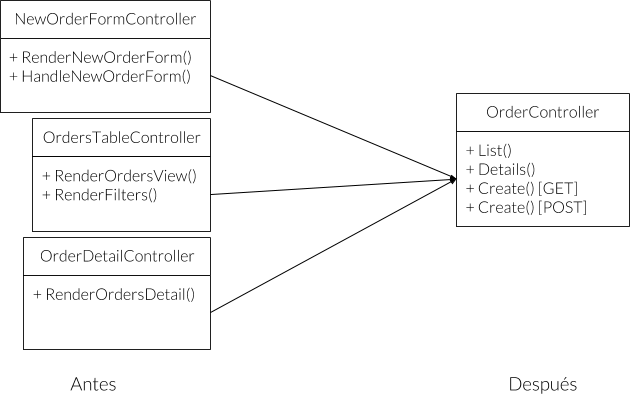
\includegraphics[width=0.7\textwidth]{controller_changes.png}
    \caption{Cambios a los controladores}
    \label{fig:controller_changes}
\end{figure}

\begin{figure}[H]
    \centering
    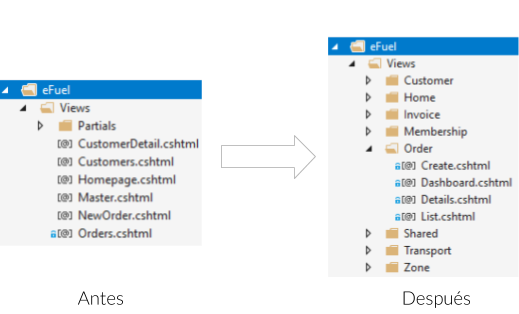
\includegraphics[width=0.7\textwidth]{views_changes.png}
    \caption{Cambios a las vistas}
    \label{fig:views_changes}
\end{figure}

Durante esta iteración también se llevó a cabo una reunión con los miembros del equipo (el dueño del producto/tutor industrial y otros integrantes del equipo de programación de la empresa) para revisar el estado de la aplicación y para evaluar el código escrito hasta el momento. Como resultado de la evaluación se realizaron varios comentarios y correcciones sobre el código para seguir las buenas prácticas y convenciones del equipo de desarrollo de la empresa.

\vspace{0.3cm}
\textbf{Actividades realizadas:}
\begin{itemize}
    \item Se cambió la estructura del código para que siguiera el patrón MVC de una mejor manera.
    \item Mejoras en la calidad del código en general. Se hizo más robusto el código al chequear cada conexión a la base de datos para capturar errores, se mejoró la eficiencia de algunas consultas a la base de datos, se cambiaron los nombres de algunas variables y métodos, se ajustaron algunos detalles con el espacado del código. Todo esto con el objetivo de seguir las buenas prácticas de la empresa y hacer el código más legible y mantenible.
\end{itemize}

\textbf{Duración:} 3 semanas.

\subsubsection{Continuación con el Módulo de Pedidos (5ta Iteración)}
En esta Iteración se continuó el desarrollo de la funcionalidad referente a los pedidos del sistema.

\vspace{0.3cm}
\textbf{Actividades realizadas:}
\begin{itemize}
    \item Implementación de la funcionalidad de crear pedido en el front end. Para esto fue necesario crear 2 métodos en el controlador de pedidos, un para mostrar el formulario y otro para chequear que los datos introducidos son válidos, también se implementó un método que, dado un cliente, devuelve la lista de fechas disponibles con los transportes y turnos disponibles. También se diseñó la vista correspondiente y se desarrolló un script de JavaScript para ir hablitando los campos del formulario a medida que se van seleccionando las opciones. Para crear un pedido se debe selccionar un cliente, al seleccionarlo el servidor envía al cliente la lista de fechas disponibles con sus transportes y turnos correspondientes, se habilita el campo de fecha, se seleccicona una fecha, se habilita el campo de transporte y se selecciona uno de los transportes disponibles, se habilita el campo de turno, se selcciona uno de los disponibles y, fianlmente se selccionan los productos del pedido. En la Figura \ref{fig:ordercreate} se muestra el formulario.
    \item Implementación de la funcionalidad exportación de la lista de pedidos desde el front end. Para esto se diseñó un método que busca la lista de pedidos (puede o no tener filtros aplicados) y genera un archivo de Excel con la información de éstos.
\end{itemize}

\begin{figure}[H]
    \centering
    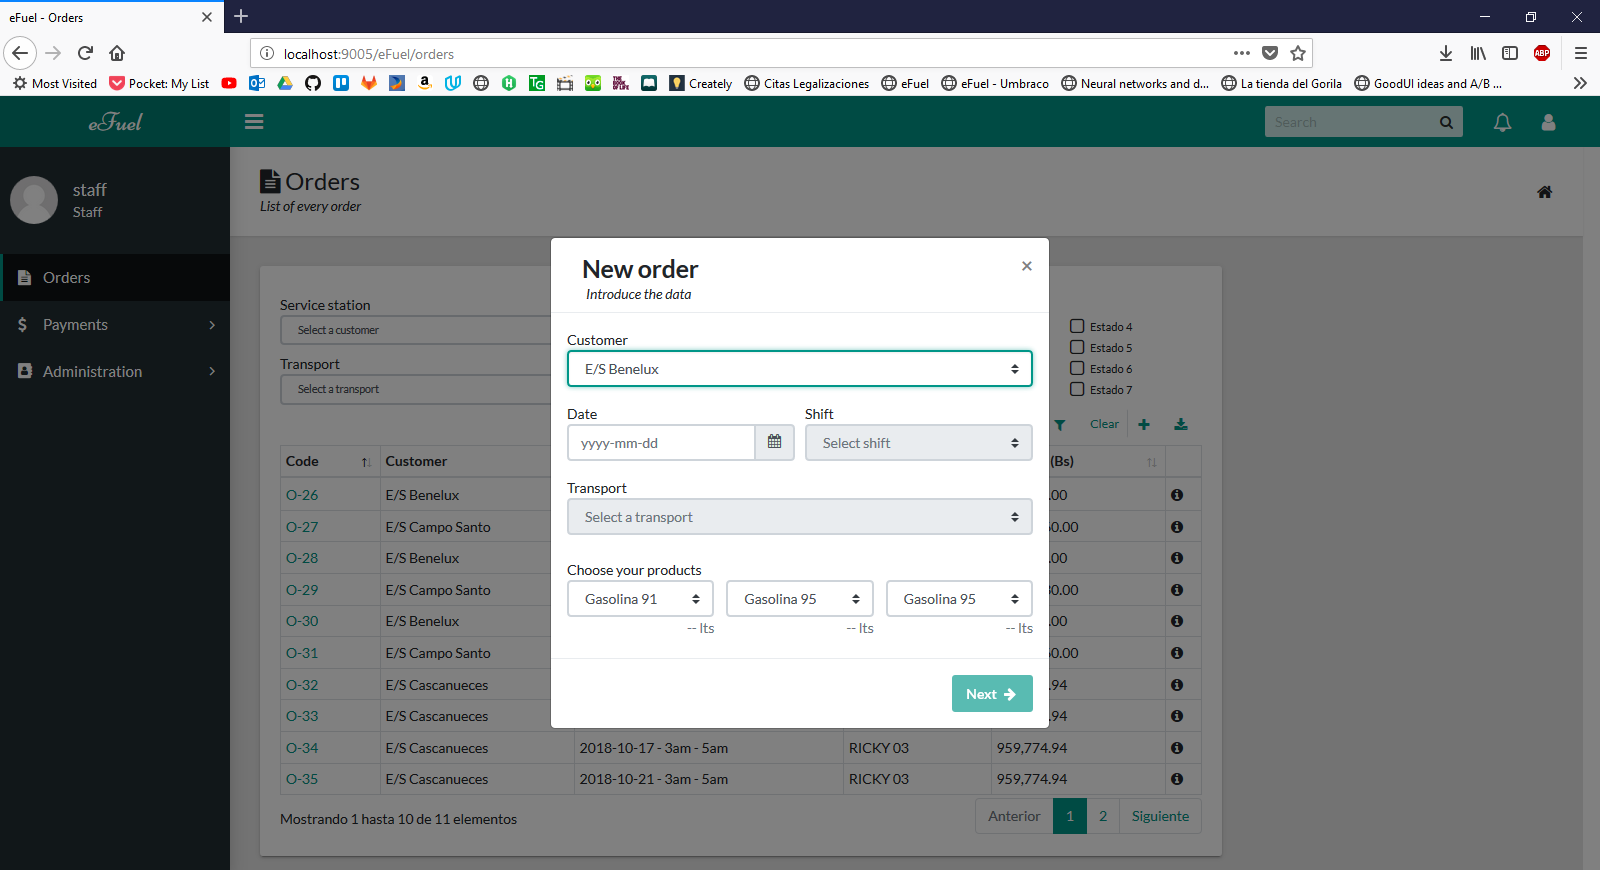
\includegraphics[width=0.7\textwidth]{./vistas/frontend/orders_create.png}
    \caption{Formulario para crear un pedido (captura)}
    \label{fig:ordercreate}
\end{figure}

\textbf{Duración:} 3 semanas.

\subsubsection{Módulo de Manejo de Usuarios e Importación (6ta Iteración)}
Ésta fue la última Iteración de desarrollo, en ella se desarrolló el módulo de manejo de usuarios y se implementó la funcionalidad de importación de algunas entidades. También se mejoraron todos los aspectos que fueron posibles del código y se empezó a desarrollar el módulo de pagos, tan solo se terminó una vista (lista de facturas).

\vspace{0.3cm}
\textbf{Actividades realizadas:}
\begin{itemize}
    \item Se definieron los tipos de usuario y los permisos por actor (customer y staff) para el front end. Para esto se creó un tipo de miembro llamado \emph{eFuel Member} desde la sección Members del back office de Umraco y luego se crearon 2 grupos de miembros: \emph{eFuel Customer} y \emph{eFuel Staff}.
    \item Implementación de funcionalidad de autenticación, inicio y cierre de sesión para el front end de la aplicación. Para esto se tuvo que agregar lógica de autenticaión en cada método de cada controlador para chequear si hay un usuario con una sesión abierta y, en ese caso, si posee los permisos necesarios.
    \item Implementación de la funcionalidad de importación de Zonas y Transportes desde archivos de Excel en el front end. Para esto se implementaron métodos en los controladores de Transportes y Zonas que se encargan de leer un archivo de Excel y de crear registros en la base de datos basados en la información de los archivos.
    \item Se implementó la funcionalidad de listado de facturas en el front end. Para esto se diseñaron el controlador y la vista correspondientes.
\end{itemize}

\textbf{Duración:} 3 semanas.

\subsection{Fase de Documentación} \label{documentation}
Esta fase duró 1 semana, en ella se elaboró un Documento de Arquitectura de Software donde se detallan los componentes y casos de uso desarrollados de la aplicación y, además, se elaboró una guía de instalación de eFuel. A lo largo de esta sección se utiliza el término \emph{vista} para referirse a una representación del sistema desde la perspectiva de un conjunto de propiedades relacionadas (a diferencia de las Vistas de MVC o de Umbraco), a menos que se indique explícitamente lo contrario.

A continuación se describe la arquitectura del software como aparece en el Documento de Arquitectura del Software desarrollado durante esta fase. El documento está basado en el modelo 4+1 de arquitectura de Phillipe Kruchten \cite{41Kruchten}, contempla la Vista de Casos de Uso, la Vista Lógica, la Vista de Implantación, la Vista de Implementación y la Vista de Datos. Adicionalmente se elaboró documentación de los componentes de Umbraco del sistema y se incorporó a este documento. Para una descripción detallada de todas las vistas elaboradas referirse al Anexo \ref{das}.


\subsubsection{Arquitectura de Software}
En esta sección se presentan los elementos importantes cada una de las vistas elaboradas para el Documento de Arquitectura del Software. Referirse al Anexo \ref{das} para ver todos los detalles elaborados.

\paragraph{Vista de Casos de Uso} En esta vista se describirá el sistema desde el punto de vista de los casos de uso. El sistema tiene 3 actores:

\begin{itemize}
    \item \emph{Admin}: administrador de eFuel. Es un usuario de Umbraco, esto es, cuenta con las credenciales para ingresar al back end de Umbraco y, además, tiene los permisos necesarios para administrar las entidades y los miembros de eFuel.
    \item \emph{Customer}: representa a una o varias estaciones de servicio. Solo tiene acceso a la información referente a las estaciones de servicio asignadas por el administrador del sistema. Es el tipo de miembro que más uso le dará al sistema.
    \item \emph{Staff}: representa a un distribuidor de combustible. Tiene acceso a la información de todas las estaciones de servicio del sistema.
\end{itemize}

A continuación, se presenta el resumen de los casos de uso del sistema.

\newcounter{magicrownumbers}
\newcommand\rownumber{\stepcounter{magicrownumbers}\arabic{magicrownumbers}}

\vspace{0.4cm}
\begin{longtable}{ | l | l | c | }
    \hline
    \rowcolor{gray!30}
    \multicolumn{1}{|c|}{ID del Caso de Uso} &
    \multicolumn{1}{|c|}{Caso de Uso} &
    \multicolumn{1}{|c|}{Actor} \\
    \hhline{===}
    \endhead

    CU-\rownumber & Iniciar sesión (Umbraco) & Admin \\ \hline
    CU-\rownumber & Consultar lista de miembros & Admin \\ \hline
    CU-\rownumber & Gestionar miembro (CRUD) & Admin \\ \hline
    CU-\rownumber & Asignar cliente/s a miembro & Admin \\ \hline
    CU-\rownumber & Remover cliente/s de miembro & Admin \\ \hline
    CU-\rownumber & Cambiar permisos de miembro & Admin \\ \hline

    CU-\rownumber & Gestionar contenido & Admin \\ \hline
    CU-\rownumber & Consultar lista de clientes & Admin \\ \hline
    CU-\rownumber & Gestionar cliente (CRUD) & Admin \\ \hline
    CU-\rownumber & Consultar lista de productos & Admin \\ \hline
    CU-\rownumber & Gestionar producto (CRUD) & Admin \\ \hline
    CU-\rownumber & Consultar lista de transportes & Admin \\ \hline
    CU-\rownumber & Gestionar transportes (CRUD) & Admin \\ \hline
    CU-\rownumber & Consultar lista de zonas & Admin \\ \hline
    CU-\rownumber & Gestionar zonas (CRUD) & Admin \\ \hline

    CU-\rownumber & Gestionar transacciones & Admin \\ \hline
    CU-\rownumber & Consultar lista de registros & Admin \\ \hline
    CU-\rownumber & Gestionar registro (CRUD) & Admin \\ \hline
    CU-\rownumber & Consultar lista de pedidos & Admin \\ \hline
    CU-\rownumber & Gestionar pedido (CRUD) & Admin \\ \hline
    CU-\rownumber & Consultar lista de detalles de pedidos & Admin \\ \hline
    CU-\rownumber & Gestionar detalle de pedido (CRUD) & Admin \\ \hline
    CU-\rownumber & Consultar lista de facturas & Admin \\ \hline
    CU-\rownumber & Gestionar factura (CRUD) & Admin \\ \hline
    
    CU-\rownumber & Registrar pago & Customer, Staff \\ \hline
    CU-\rownumber & Asignar pago a pedido & Customer, Staff \\ \hline
    CU-\rownumber & Consultar lista de pagos & Customer, Staff \\ \hline
    CU-\rownumber & Consultar pagos pendientes & Customer, Staff \\ \hline
    CU-\rownumber & Consultar pagos realizados & Customer, Staff \\ \hline
    CU-\rownumber & Registrar pago & Customer, Staff \\ \hline
    CU-\rownumber & Importar lista de facturas & Staff \\ \hline
    
    CU-\rownumber & Consultar lista de cobros & Admin \\ \hline
    CU-\rownumber & Gestionar cobro (CRUD) & Admin \\ \hline
    CU-\rownumber & Consultar lista de detalles de cobros & Admin \\ \hline
    CU-\rownumber & Gestionar detalle de cobro (CRUD) & Admin \\ \hline

    CU-\rownumber & Iniciar sesión (eFuel) & Customer, Staff \\ \hline
    CU-\rownumber & Consultar lista de pedidos & Customer, Staff \\ \hline
    CU-\rownumber & Consultar pedido & Customer, Staff \\ \hline
    CU-\rownumber & Filtrar lista de pedidos & Customer, Staff \\ \hline
    CU-\rownumber & Exportar lista de pedidos & Customer, Staff \\ \hline
    CU-\rownumber & Crear pedido & Customer, Staff \\ \hline
    CU-\rownumber & Seleccionar cliente & Customer, Staff \\ \hline
    CU-\rownumber & Seleccionar fecha & Customer, Staff \\ \hline
    CU-\rownumber & Seleccionar turno  & Customer, Staff \\ \hline
    CU-\rownumber & Seleccionar transporte  & Customer, Staff \\ \hline
    CU-\rownumber & Seleccionar productos & Customer, Staff \\ \hline

    CU-\rownumber & Consultar lista de facturas & Customer, Staff \\ \hline

    CU-\rownumber & Consultar lista de clientes & Customer, Staff \\ \hline
    CU-\rownumber & Consultar cliente & Customer, Staff \\ \hline
    CU-\rownumber & Consultar pedidos de cliente & Customer, Staff \\ \hline
    CU-\rownumber & Importar lista de clientes & Staff \\ \hline

    CU-\rownumber & Consultar lista de transportes & Customer, Staff \\ \hline

    CU-\rownumber & Importar lista de transportes & Staff \\ \hline

    CU-\rownumber & Consultar lista de zonas & Customer, Staff \\ \hline

    CU-\rownumber & Importar lista de zonas & Staff \\ \hline

    CU-\rownumber & Importar lista de despachos & Staff \\ \hline

    \caption{Resumen de casos de uso eFuel}
    \label{tab:casosDeUsoArq}
\end{longtable}

La Figura \ref{fig:cu_admin_administracion} muestra los casos de uso del actor \textit{Admin} del Módulo de Administración.
\begin{figure}[H]
    \centering
    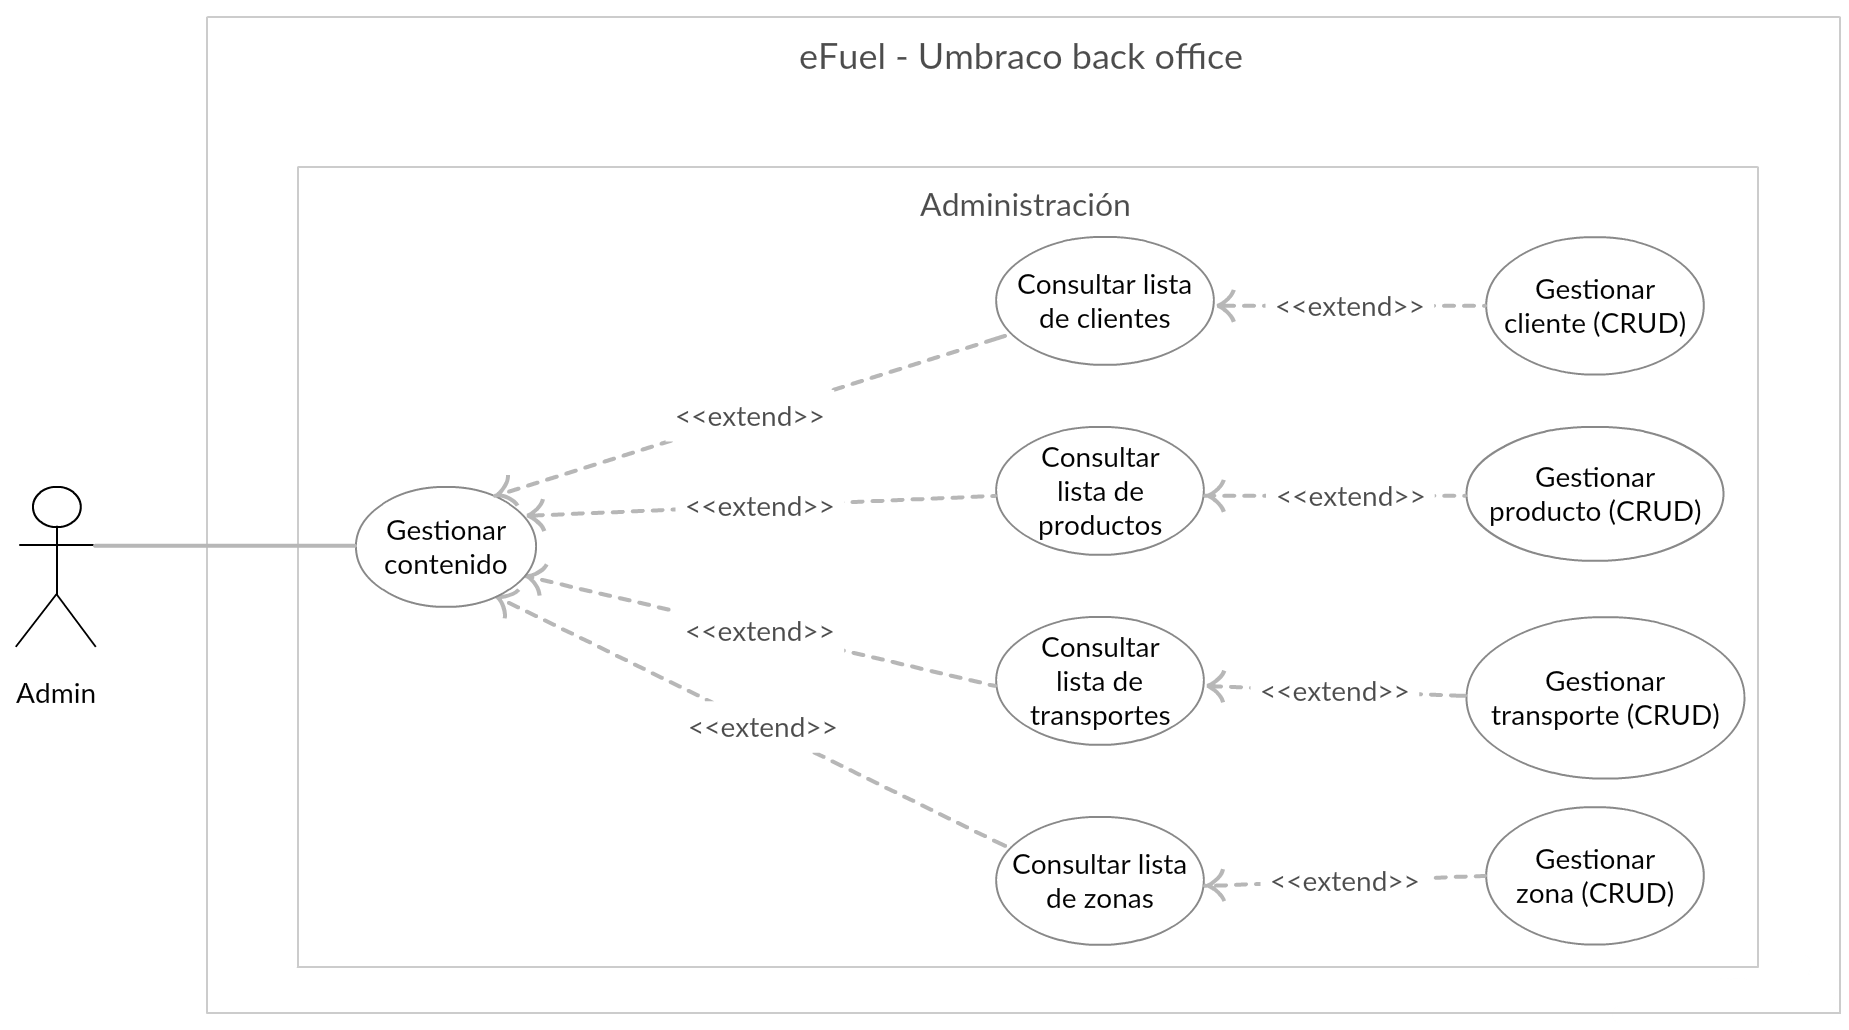
\includegraphics[width=\textwidth]{cu_admin_administracion.png}
    \caption{Casos de Uso Back office - Módulo Administración}
    \label{fig:cu_admin_administracion}
\end{figure}

\newpage
La Figura \ref{fig:cu_admin_pedidos_pagos} muestra los casos de uso del actor \textit{Admin} de los Módulos de Pedidos y Pagos.
\begin{figure}[H]
    \centering
    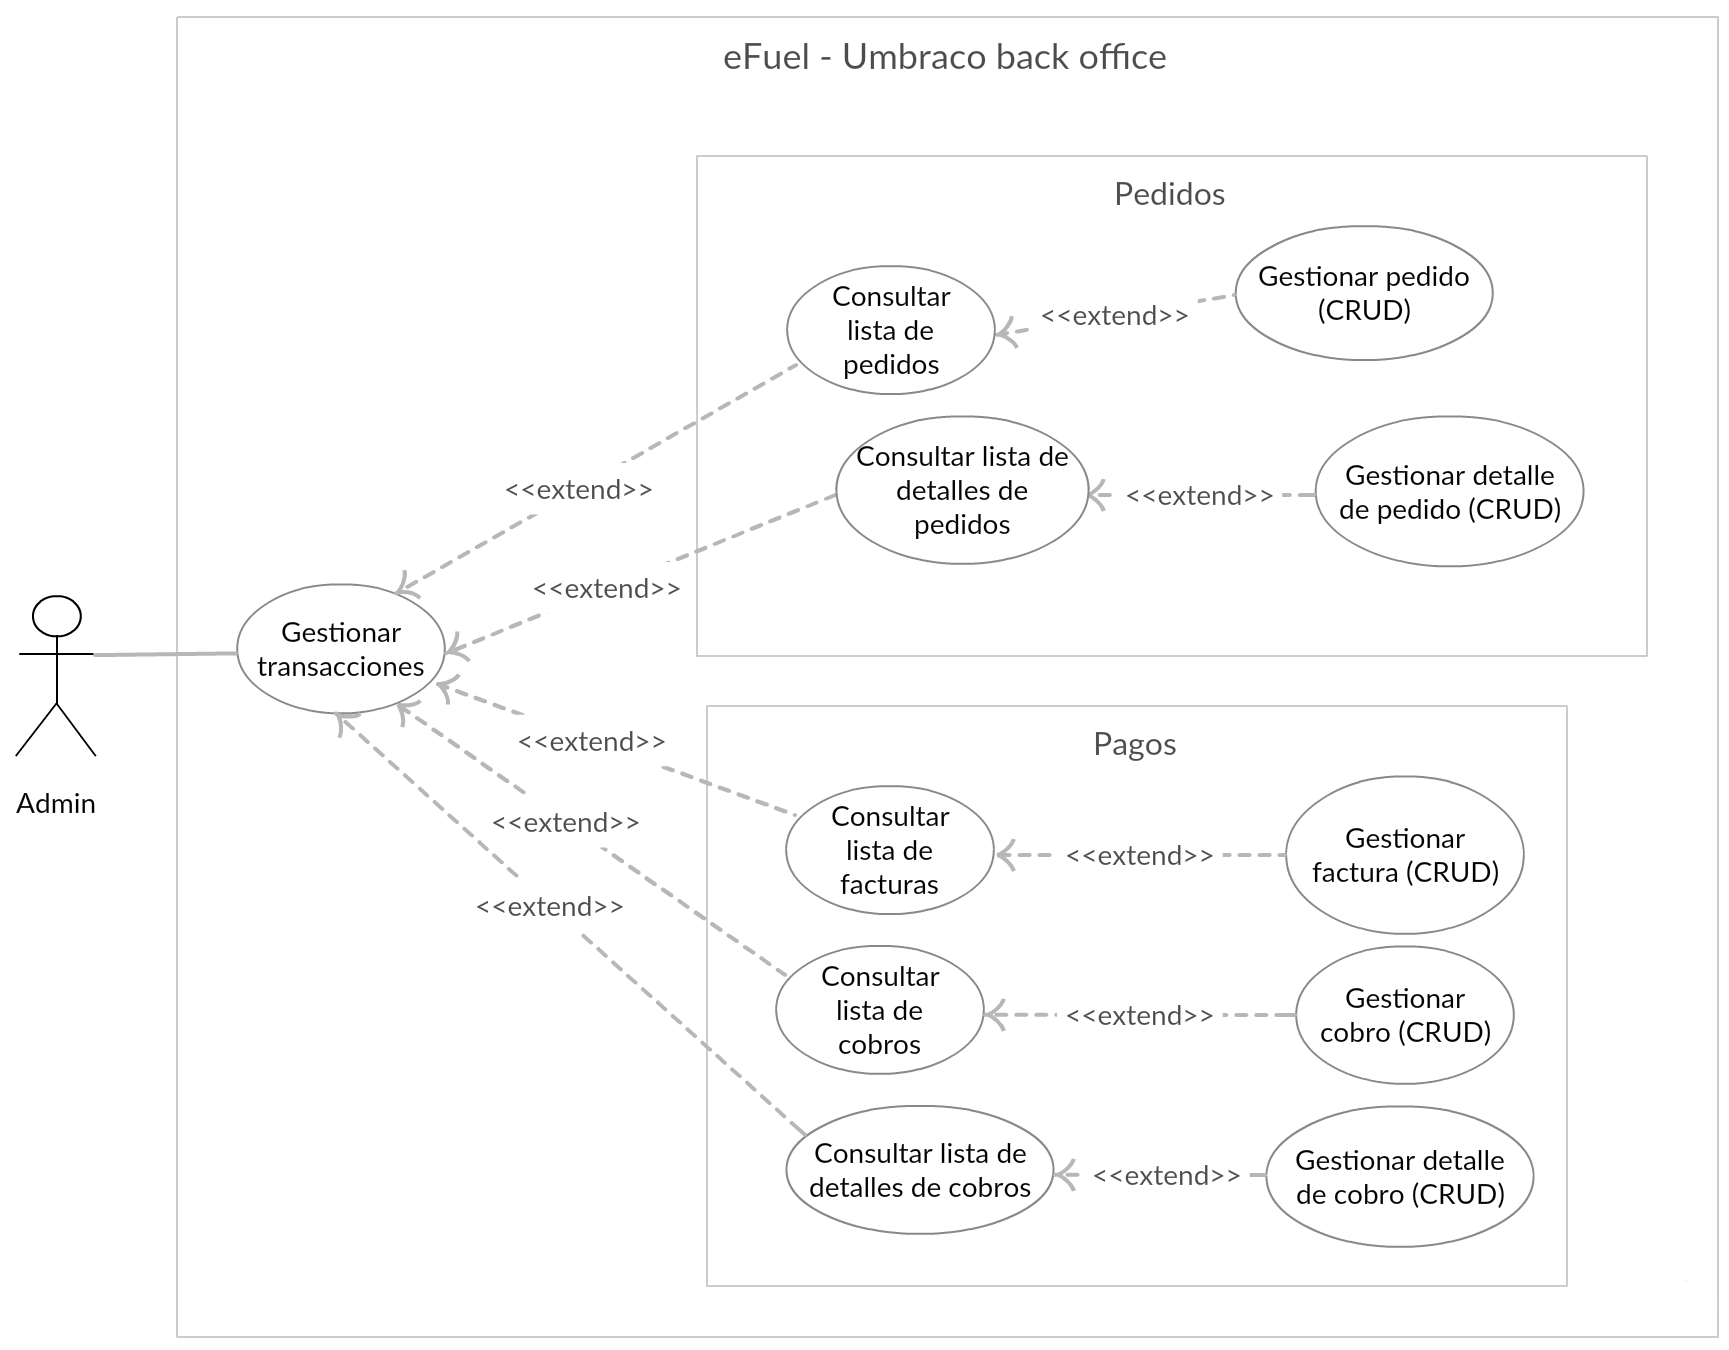
\includegraphics[width=0.9\textwidth]{cu_admin_pedidos_pagos.png}
    \caption{Casos de Uso Back office - Módulos Pedidos y Pagos}
    \label{fig:cu_admin_pedidos_pagos}
\end{figure}

\newpage
La Figura \ref{fig:cu_admin_seguridad} muestra los casos de uso del actor \textit{Admin} del Módulo de Seguridad.
\begin{figure}[H]
    \centering
    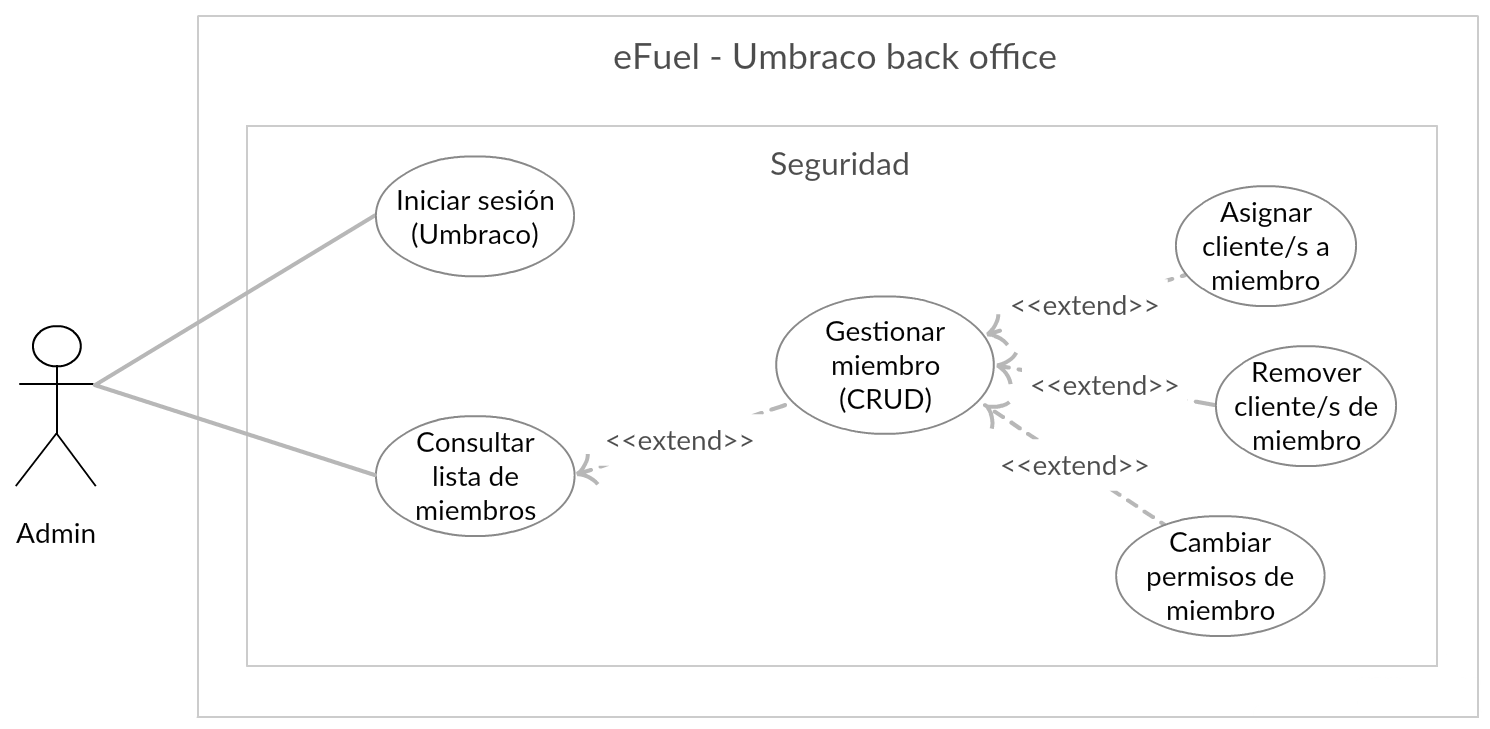
\includegraphics[width=0.9\textwidth]{cu_admin_seguridad.png}
    \caption{Casos de Uso Back office - Módulo Seguridad}
    \label{fig:cu_admin_seguridad}
\end{figure}
\vspace*{\fill}

\newpage
La Figura \ref{fig:cu_customer_staff_pedidos} muestra los casos de uso de los actores \textit{Staff} y \textit{Customer} de los Módulos de Pedidos y Seguridad.
\begin{figure}[H]
    \centering
    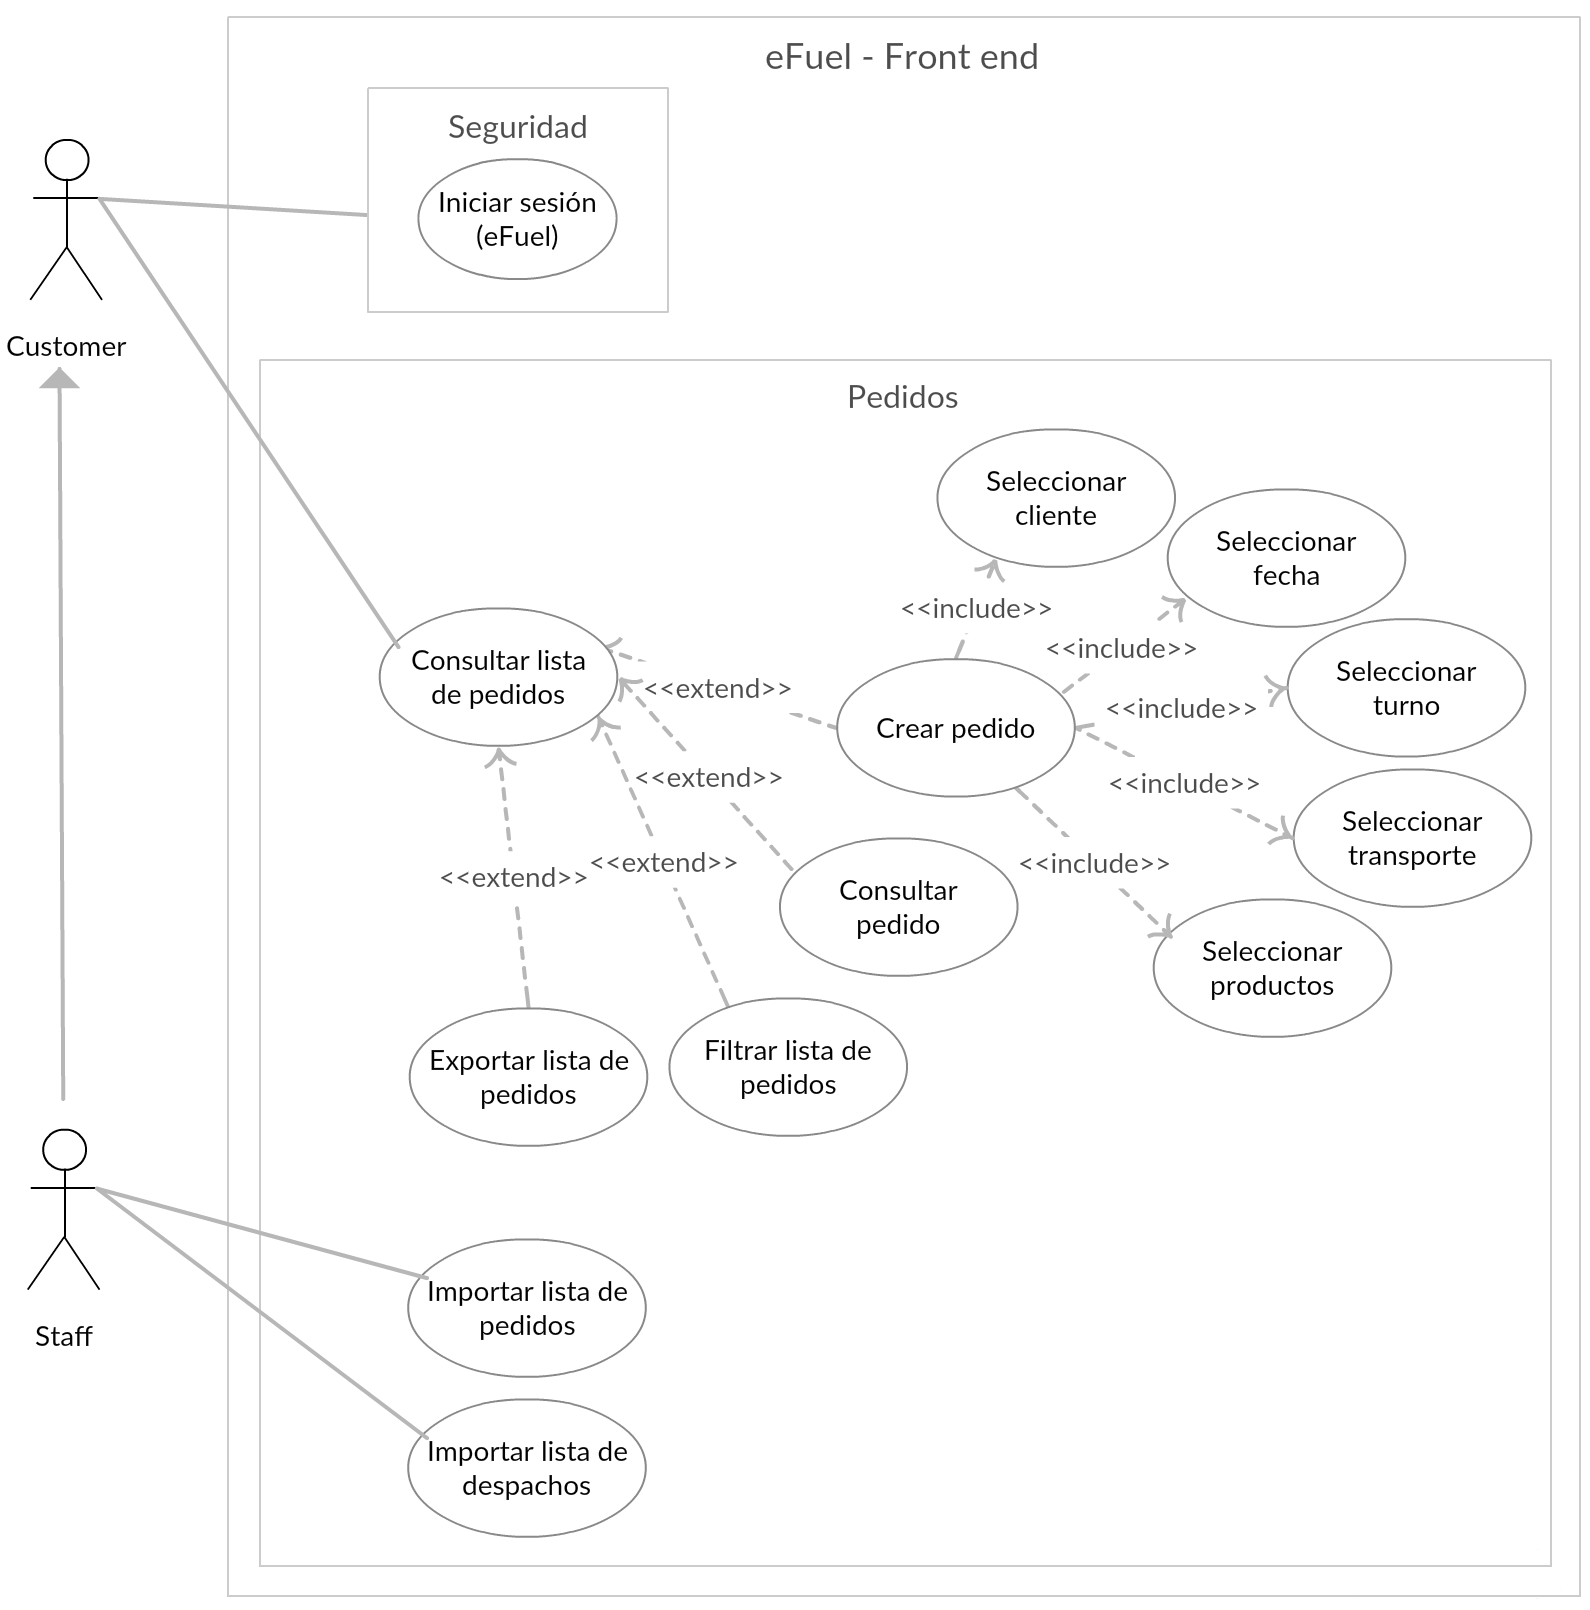
\includegraphics[width=\textwidth]{cu_customer_staff_pedidos_seguridad.png}
    \caption{Casos de Uso Front end - Módulos Pedidos y Seguridad}
    \label{fig:cu_customer_staff_pedidos}
\end{figure}
\vspace*{\fill}

\newpage
La Figura \ref{fig:cu_customer_staff_pagos} muestra los casos de uso de los actores \textit{Staff} y \textit{Customer} del Módulo de Pagos.
\begin{figure}[H]
    \centering
    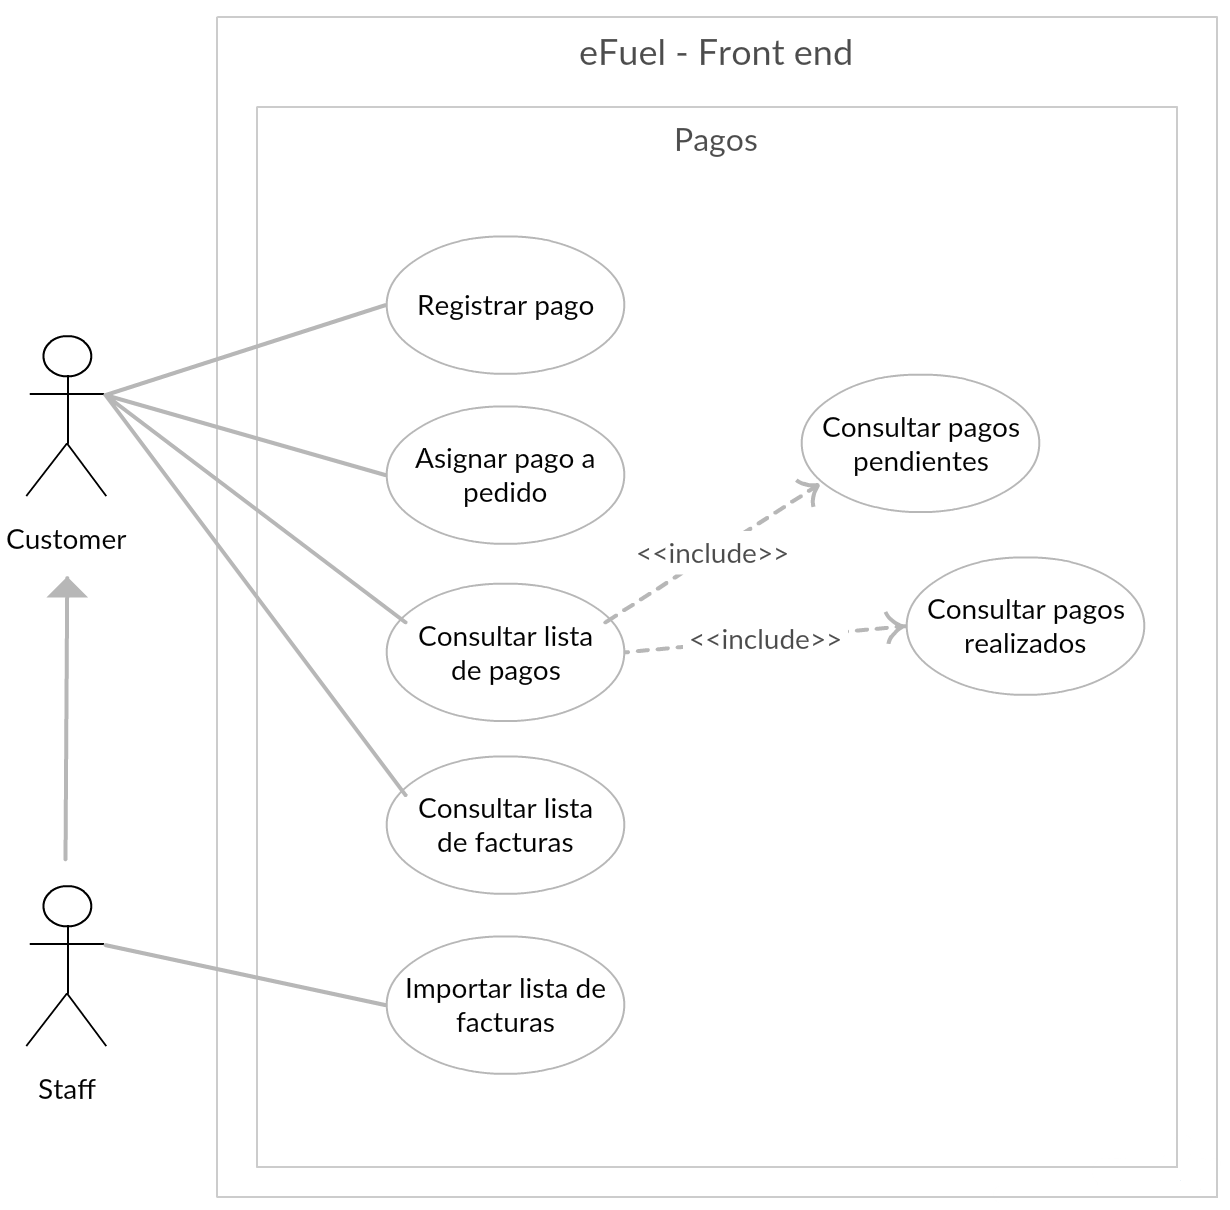
\includegraphics[width=\textwidth]{cu_customer_staff_pagos.png}
    \caption{Casos de Uso Front end - Módulo Pagos}
    \label{fig:cu_customer_staff_pagos}
\end{figure}
\vspace*{\fill}

\newpage
La Figura \ref{fig:cu_customer_staff_administracion} muestra los casos de uso de los actores \textit{Staff} y \textit{Customer} del Módulo de Administración.
\begin{figure}[H]
    \centering
    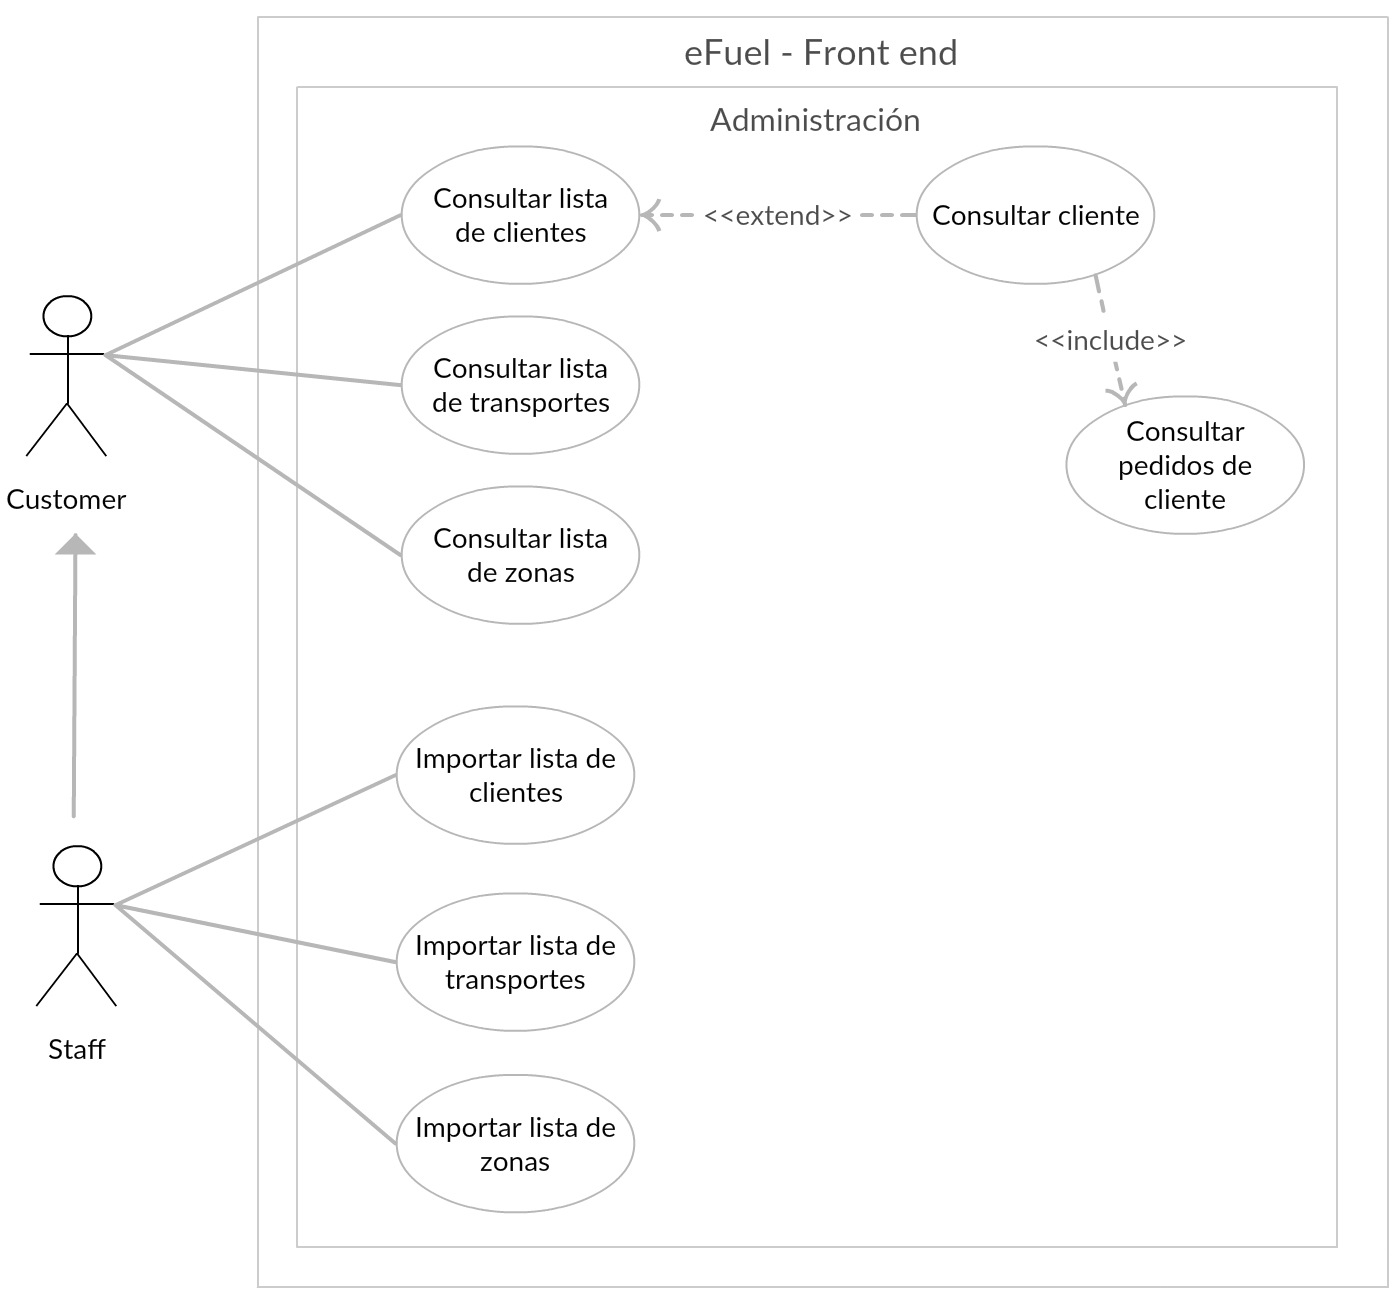
\includegraphics[width=\textwidth]{cu_customer_staff_administracion.png}
    \caption{Casos de Uso Front end - Módulo Administración}
    \label{fig:cu_customer_staff_administracion}
\end{figure}

\newpage
\paragraph{Vista Lógica} se muestran 2 diagramas que describen, de manera estática, la estructura del sistema y su interacción con entidades externas.

\subparagraph*{Diagrama Conceptual (Modelo de Dominio)} este diagrama muestra la interacción de eFuel con sistemas y agentes externos.
\begin{figure}[H]
    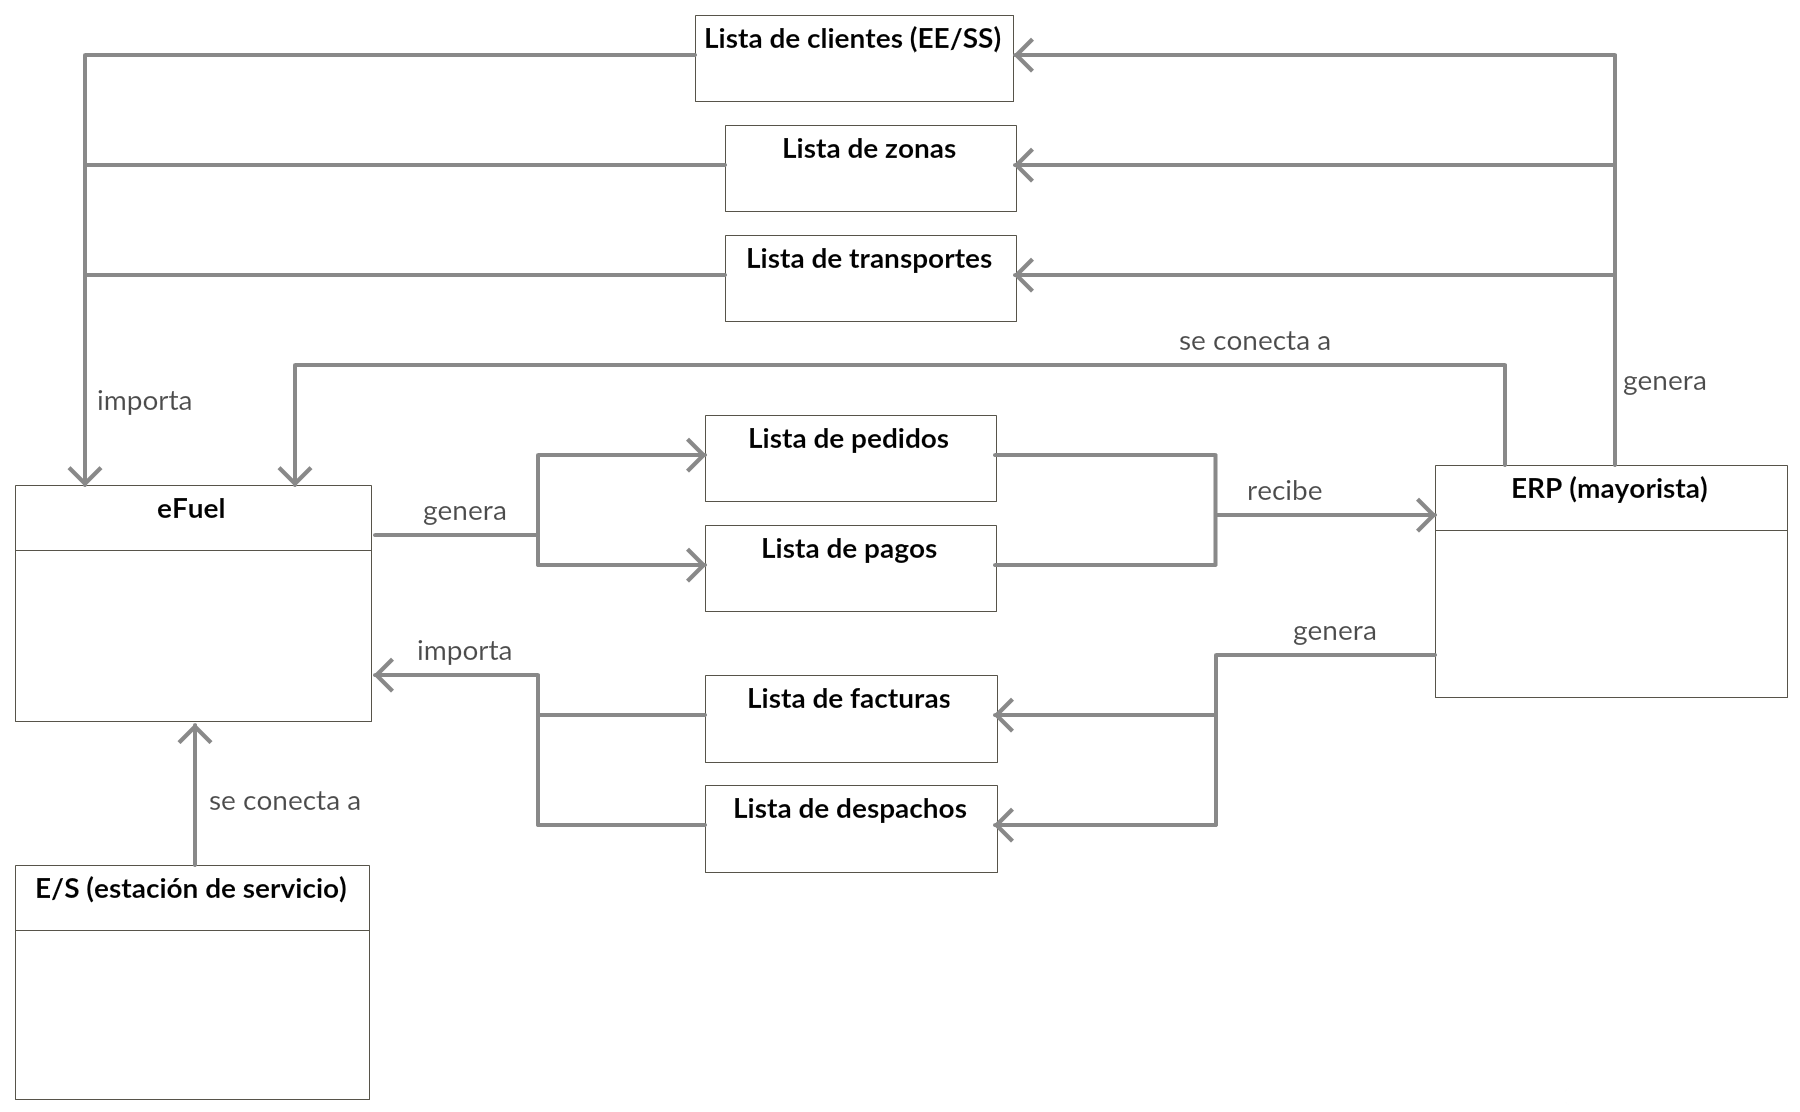
\includegraphics[width=\textwidth]{domain_model.png}
    \caption{Modelo de Dominio}
    \label{fig:domain_model}
    \centering
\end{figure}

\subparagraph*{Diagrama de Clases} a continuación se muestra un diagrama donde están representadas las principales entidades del sistema y las relaciones entre ellas. Las tablas con los bordes punteados son Doctypes de Umbraco representados como clases y los de línea continua son las clases principales del sistema (no son Doctypes de Umbraco).

\begin{figure}[H]
    \centering
    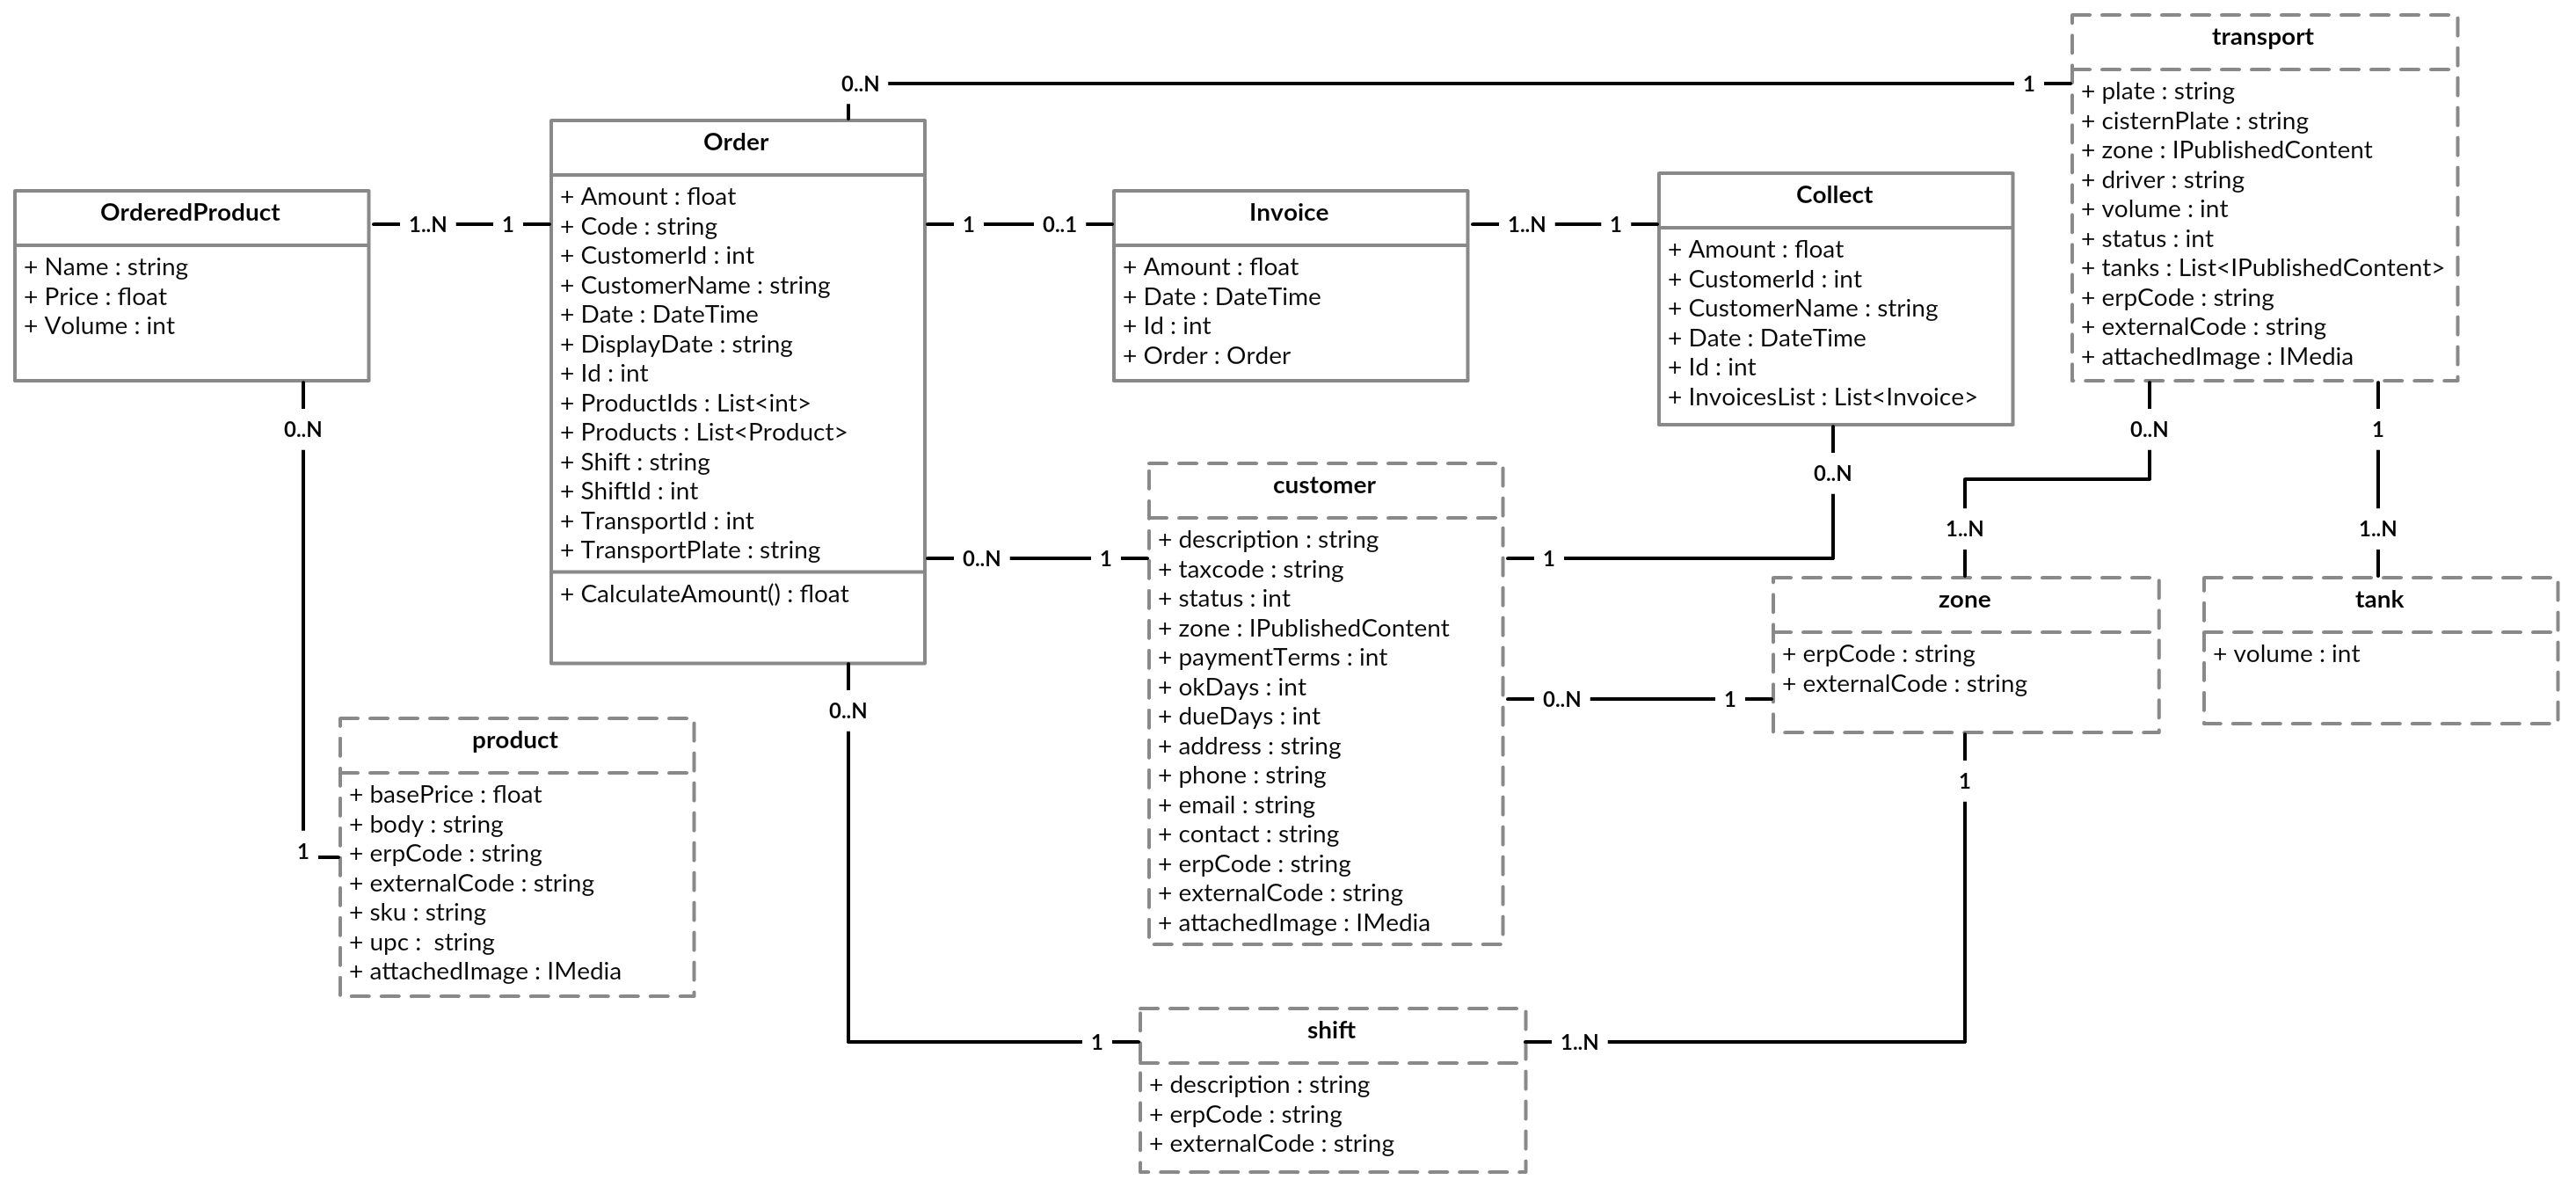
\includegraphics[width=0.7\textwidth]{class_diagram.png}
    \caption{Diagrama de Clases de las entidades principales}
    \label{fig:class_diagram_main}
\end{figure}

\paragraph{Vista de Implantación} esta vista muestra los dispositivos y artefactos necesarios para la implantación del sistema.

\begin{figure}[H]
    \centering
    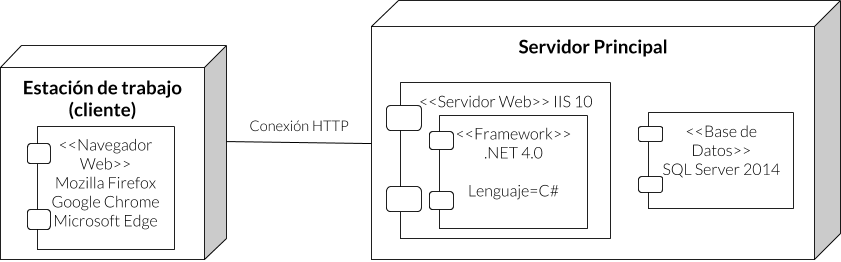
\includegraphics[width=\textwidth]{diagrama_implantacion.png}
    \caption{Diagrama de Despliegue}
    \label{fig:diagrama_implantacion}
\end{figure}

\paragraph{Vista de Implementación} esta vista hace énfasis sobre la organización de los módulos de software en el ambiente de desarrollo, en la terminología de Visual Studio (introducida en el Marco Tecnológico) estos módulos se conocen como "proyectos". La arquitectura de software desarrollada se diseñó basándose en la arquitectura MVC. A continuación se muestra una descripción de los proyectos de la solución de Visual Studio, seguido por el Diagrama de Componentes del sistema.

\subparagraph*{Módulos de eFuel} El proyecto está compuesto por 3 módulos:
\begin{itemize}
    \item \texttt{EF\_API}: contiene los controladores usados para implementar los servicios web. Estos controladores heredan de la clase \texttt{UmbracoApiController} y su función es buscar datos (normalmente listas) y devolverlos en formato JSON al cliente. Se creó un controlador por cada entidad principal del sistema (clientes, transportes, órdenes, etc).
    \item \texttt{EF\_Core}: contiene los controladores del patrón MVC, los manejadores de rutas (Route Handlers) para éstos y los modelos que sirven para interactuar con la base de datos. Los controladores de este módulo heredan de la clase \texttt{SurfaceController} y su función es, básicamente, buscar datos y devolver vistas (esto es, vistas del patrón MVC). Hay un controlador por cada tipo de entidad principal del sistema (clientes, transportes, órdenes, etc).
    \item \texttt{EF\_Miscelaneous}: contiene todos los archivos que implementan las Vistas del patrón MVC, esto es, las vistas de Umbraco (archivos de HTML, ver Sección \ref{umbracoView}), los archivos de estilo (CSS) y los scripts del front end (JavaScript). Además contiene los archivos de configuración de Fluidity.
\end{itemize}

\subparagraph*{Diagrama de Componentes} el usuario introduce un URL, el componente \texttt{eFuel\-RouteHandler} se encarga de asociar un URL con un Controlador para llamarlo, el Controlador realiza sus tareas y devuelve una Vista (del patrón MVC) o datos, dependiendo de si es un \texttt{SurfaceController} o de un \texttt{UmbracoApiController}.

\begin{figure}[H]
    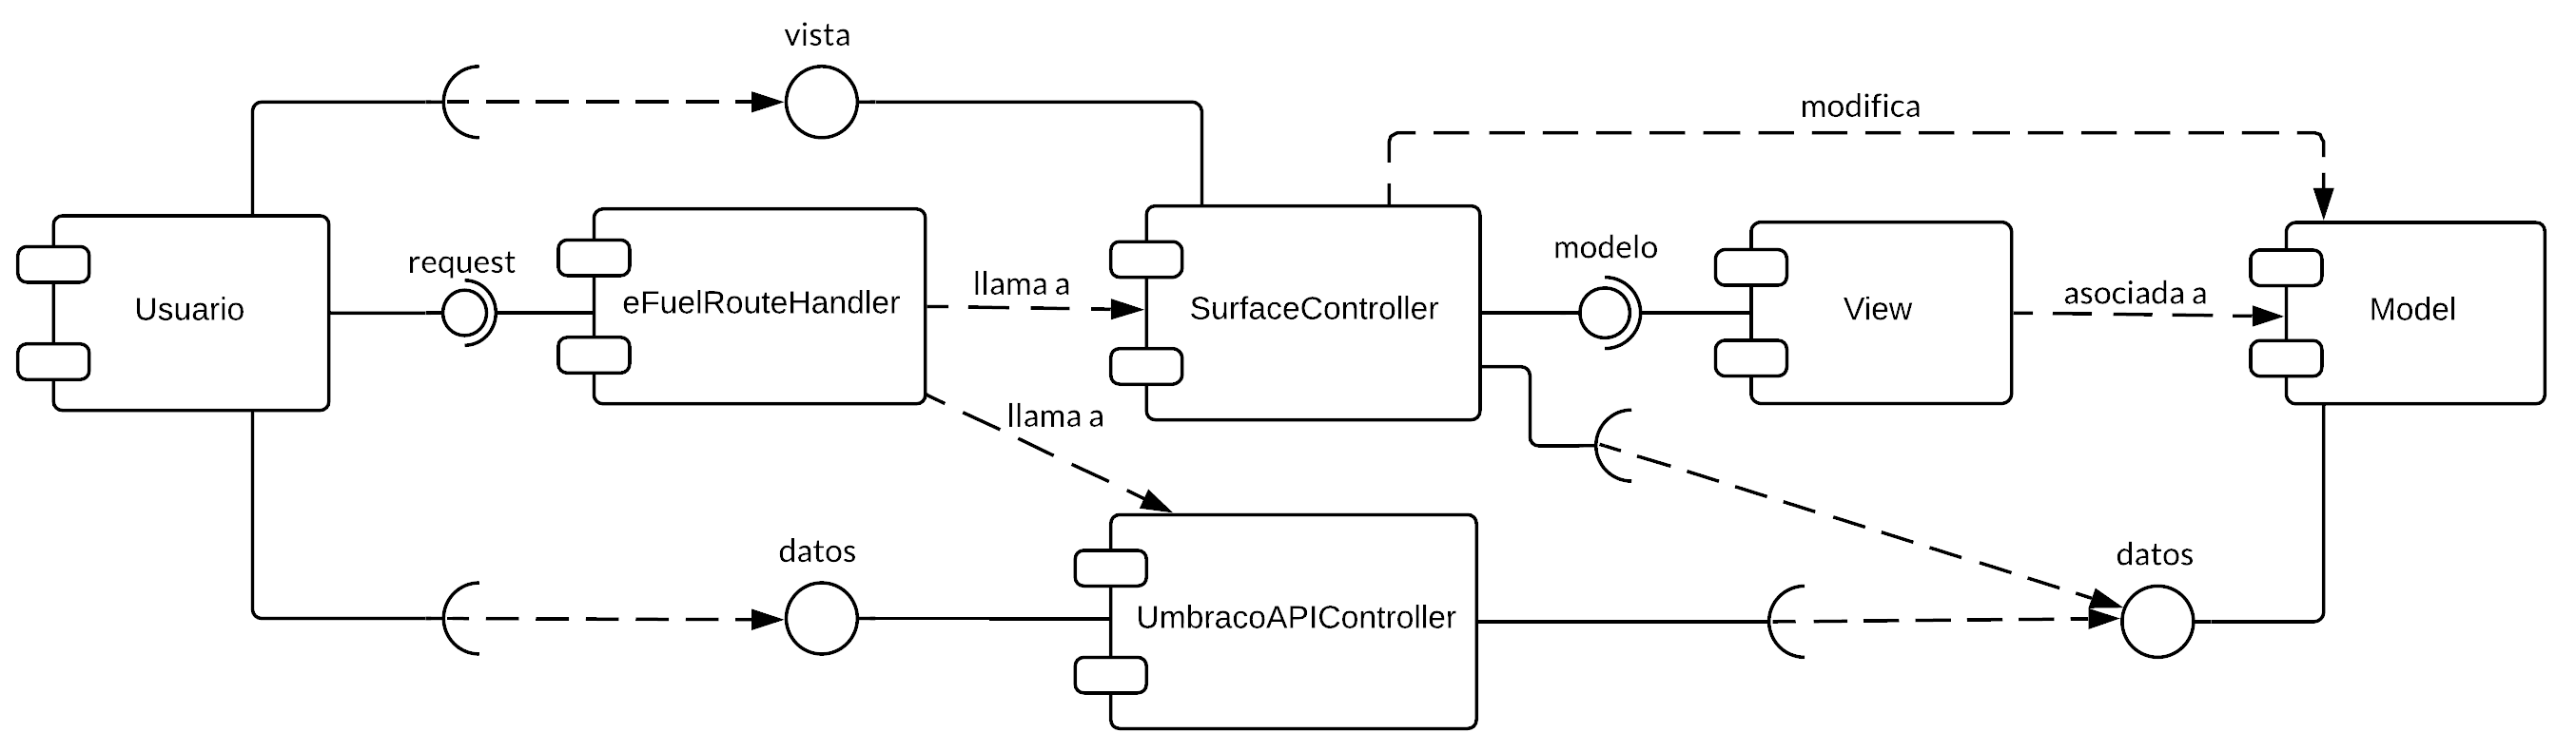
\includegraphics[width=\textwidth]{component_diagram.png}
    \caption{Diagrama de Componentes}
    \label{fig:component_diagram}
    \centering
\end{figure}

\paragraph{Componentes de Umbraco} se documenta la estructura de los componentes desarrollados en el back office de Umbraco. Primero se muestra una tabla con la lista de todas las vistas de Umbraco desarrolladas para el sistema, luego una tabla con los Doctypes y finalmente una tabla con los Data Types diseñados para eFuel.

\begin{longtable}{ | p{5.5em} | p{7em} | p{15em} | c | }
    \hline
    \rowcolor{gray!30}
    \multicolumn{1}{|c|}{Modelo} &
    \multicolumn{1}{|c|}{Nombre} &
    \multicolumn{1}{|c|}{Descripción} &
    \multicolumn{1}{|c|}{Partial View} \\
    \hhline{====}
    \endhead

    \hline
    \endfoot

    \endlastfoot

    Customer
        & Dashboard & Panel con las acciones principales que se pueden realizar sobre los clientes & - \\
    \cline{2-4}
        & Details & Información detallada de un cliente & - \\
    \cline{2-4}
        & Edit & Formulario para editar la información de un cliente & \checkmark \\
    \cline{2-4}
        & List & Tabla con todos los clientes que puede ver el usuario & \checkmark \\
    \hline

    Home
        & Dashboard & Mensaje de bienvenida (eventualmente debe mostrar las opciones más importantes del sistema) & - \\
    \hline

    Invoice
        & Dashboard & Panel con las acciones principales que se pueden realizar sobre las facturas & - \\
    \cline{2-4}
        & List & Tabla con las facturas & \checkmark \\
    \hline

    Membership
        & Index & Página de inicio de sesión & - \\
    \hline

    Order
        & Create & Formulario para crear un nuevo pedido & \checkmark \\
    \cline{2-4}
        & Dashboard & Panel con las acciones principales que se pueden realizar sobre los pedidos & - \\
    \cline{2-4}
        & Details & Información detallada de un pedido & - \\
    \cline{2-4}
        & List & Tabla con todos los pedidos que puede ver el usuario junto con los filtros y opciones de exportar la lista, crear un nuevo pedido y filtrar la lista de pedidos & \checkmark \\
    \hline

    Shared
        & AppTitle & Título de la página actual & \checkmark \\
    \cline{2-4}
        & Breadcrumbs & Cadena de enlaces a las páginas superiores a la página actual & \checkmark \\
    \cline{2-4}
        & LoginForm & Formulario de inicio de sesión & \checkmark \\
    \cline{2-4}
        & LogoutButton & Botón de cerrar sesión & \checkmark \\
    \cline{2-4}
        & Master & Estructura del sitio que es común a todas las páginas del sitio (excepto la página de inicio de sesión). Barra de navegación, barra lateral, título, etc. & - \\
    \cline{2-4}
        & Navbar & Barra de navegación superior & \checkmark \\
    \cline{2-4}
        & Sidebar & Barra de navegación lateral, contiene las secciones del sitio & \checkmark \\
    \hline

    Transport
        & Dashboard & Panel con las acciones principales que se pueden realizar sobre los transportes & - \\
    \cline{2-4}
        & Details & Información detallada de un transporte & - \\
    \cline{2-4}
        & Import & Formulario para importar una lista transportes & \checkmark \\
    \cline{2-4}
        & List & Tabla con los transportes que puede ver el usuario & \checkmark \\
    \hline

    Zone
        & Dashboard & Panel con las acciones principales que se pueden realizar sobre las zonas & - \\
    \cline{2-4}
        & Import & Formulario para importar una lista zonas & \checkmark \\
    \cline{2-4}
        & List & Tabla con las zonas que puede ver el usuario & \checkmark \\
    \hline

    \caption{Vistas del front end}
    \label{table:vistas}
\end{longtable}

\begin{longtable}{ | p{5em} | l | l | }
    \hline
    \rowcolor{gray!30}
    \multicolumn{1}{|c|}{Doctype} &
    \multicolumn{1}{|c|}{Propiedades} &
    \multicolumn{1}{|c|}{Datatype} \\
    \hline
    \endhead

    \hline
    \endfoot

    \endlastfoot

    Cliente
        & Descripción & Textarea \\
        \cline{2-3}
        & Código de impuestos & Textstring \\
        \cline{2-3}
        & Estado & Customer status \\
        \cline{2-3}
        & Zona & Zone node picker \\
        \cline{2-3}
        & Forma de pago & Payment terms \\
        \cline{2-3}
        & Ok days & Numeric \\
        \cline{2-3}
        & Due days & Numeric \\
        \cline{2-3}
        & Dirección & Textstring \\
        \cline{2-3}
        & Teléfono & Textstring \\
        \cline{2-3}
        & Correo & Email address \\
        \cline{2-3}
        & Contacto & Textstring \\
        \cline{2-3}
        & Código ERP & Textstring \\
        \cline{2-3}
        & Código externo & Textstring \\
        \cline{2-3}
        & Imagen & Attached images \\
    \hline

    Producto
        & Precio base & Decimal \\
        \cline{2-3}
        & Descripción & Textarea \\
        \cline{2-3}
        & Código ERP & Textstring \\
        \cline{2-3}
        & Código externo & Textstring \\
        \cline{2-3}
        & SKU & Textstring \\
        \cline{2-3}
        & EAN/UPC & EAN-UPC \\
        \cline{2-3}
        & Imagen & Attached images \\
    \hline

    Tanque
        & Volumen & Numeric \\
    \hline

    Transporte
        & Placa chuto & Textstring \\
        \cline{2-3}
        & Placa cisterna & Textstring \\
        \cline{2-3}
        & Zona & Zone node picker \\
        \cline{2-3}
        & Nombre del conductor & Textstring \\
        \cline{2-3}
        & Volumen total & Numeric \\
        \cline{2-3}
        & Estado & Transport status \\
        \cline{2-3}
        & Tanques & Tank list \\
        \cline{2-3}
        & Código ERP & Textstring \\
        \cline{2-3}
        & Código externo & Textstring \\
        \cline{2-3}
        & Imagen & Attached images \\
    \hline

    Turno
        & Descripción & Textstring \\
        \cline{2-3}
        & Código ERP & Textstring \\
        \cline{2-3}
        & Código externo & Textstring \\
    \hline

    Zona
        & Código ERP & Textstring \\
        \cline{2-3}
        & Código externo & Textstring \\
    \hline

    \caption{Doctypes}
    \label{table:doctypes}
\end{longtable}

\begin{longtable}{  l | l  }
    \hline\hline
    \rowcolor{gray!30}
    \textbf{Datatype} & \textbf{Uso} \\
    \hline\hline
    \endhead

    \hline
    \endfoot

    \endlastfoot

    Collect picker & Seleccionar un cobro \\
    Customer picker & Seleccionar un cliente \\
    Invoice picker & Seleccionar una factura \\
    Order picker & Seleccionar un pedido \\
    Product picker & Seleccionar un producto \\
    Shift picker & Seleccionar un turno \\
    Tank picker & Seleccionar un tanque \\
    Transport picker & Seleccionar un transporte del árbol de contenido \\
    Customer node picker & Seleccionar el nodo de un cliente del árbol de contenido \\
    Zone node picker & Seleccionar el nodo de una zona del árbol de contenido \\
    Attached images & Seleccionar una imagen \\
    Customer status & Elegir uno de los estados del cliente \\
    EAN-UPC & Introducir el código EAN o UPC de un producto \\
    Email address & Introducir un correo electrónico \\
    On Off & Elegir uno de 2 estados: on u off \\
    Payment terms & ELegir una forma de pago \\
    Tank list & Agregar o eliminar tanques a un transporte \\
    Textstring max65 & Introducir texto de máximo 65 caracteres \\
    Transport status & Seleccionar el estado de un transporte \\

    \hline

    \caption{Datatypes}
    \label{table:datatypes}
\end{longtable}

\paragraph{Vista de Datos} se documenta la estructura de las entidades creadas fuera de Umbraco para la base de datos.
\begin{figure}[H]
    \centering
    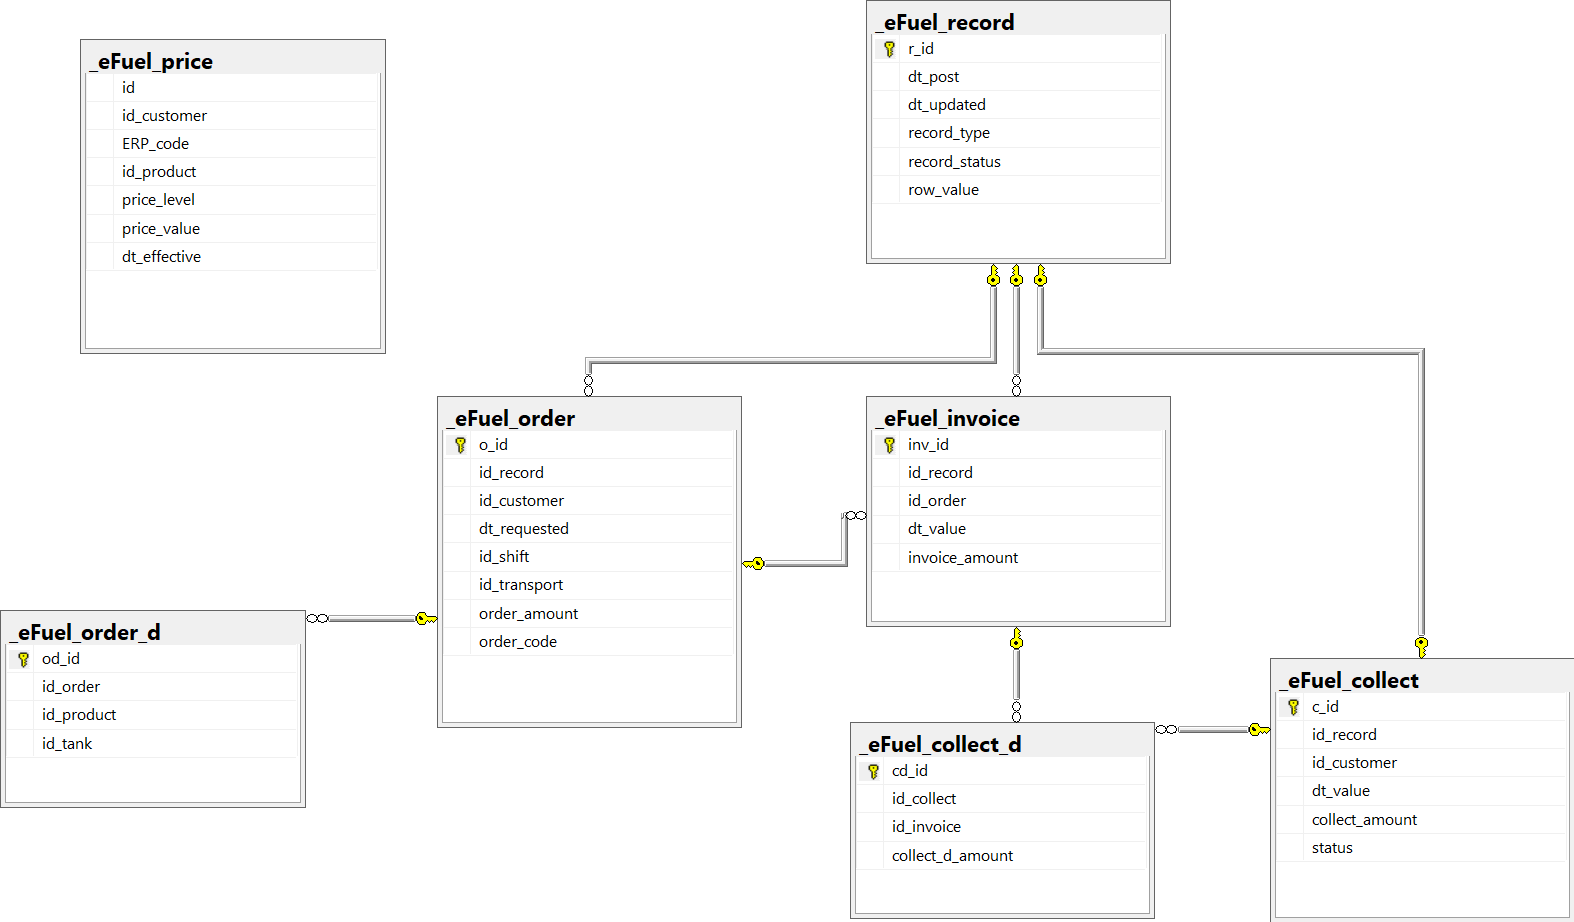
\includegraphics[width=\textwidth]{er_diagram.png}
    \caption{Diagrama ER}
    \label{fig:er_diagram}
\end{figure}
    \chapter{Resultados} \label{results}


\section{Casos de Uso} \label{useCases}


    \chapter*{Conclusiones y Recomendaciones}
Durante el desarrollo hubo algunos retrasos y refactorizaciones en el código (de hecho no se pudo completar la funcionalidad del módulo de conciliación de pagos), esto se puede atribuir a varios factores. Los conocimientos adquiridos durante la fase de inducción no fueron suficientes para llevar un ritmo de desarrollo adecuado, falta de comunicación del pasante con el equipo de apoyo de la empresa, poca revisión del progreso del proyecto por parte del tutor industrial/dueño del producto.

Es de esperarse que cuando se embarca en un proyecto de desarrollo nuevo se deban obtener habilidades nuevas y aprender sobre nuevas tecnologías, sobre todo al nivel de pasante con poca experiencia laboral. Aliviar este inconveniente era el objetivo de la fase de inducción, sin embargo, ese objetivo no fue alcanzado de manera satisfactoria.


Sabiendo esto, hay que resaltar la importancia de generar documentos que ayuden a plasmar una visión del sistema para que todos los actores tengan claro qué hace el sistema y cómo se espera que lo haga, de esta manera el desarrollo será más fluido.


Por otro lado, al enfrentarse con nuevas tecnologías y conceptos es importante saber consultar tanto fuentes de información (documentación, libros, etc) como al equipo de trabajo, ya que muchas veces otra persona del equipo ha resolvido problemas similares o tiene experiencia con las tecnologías utilizadas y puede ayudar a avanzar con el desarrollo de una manera importante. Hay que saber cómo y dónde buscar información.

El pasante obtuvo muchas enseñanzas tanto a nivel tecnológico como a nivel personal, sobre todo con respecto a lo que implica el proceso de desarrollo de software desde la concepción hasta la entrega del producto. La documentación y la planificación son integrales para poder crear un producto de buena calidad y en tiempos deseables, se debe tener siempre en mente que muchos componentes del software cambian a lo largo del desarrollo, también es importante saber cuando se debe pedir ayuda a otras personas del equipo para poder agilizar el desarrollo de la mejor manera posible.

El proyecto de pasantía fue una oportunidad para poner en práctica muchos conceptos y teorías aprendidas en la carrera, para reforzar y complementarlos, para entender por qué son importantes pero también que la teoría y la práctica pueden ser muy diferentes y es el trabajo del ingeniero reconciliar las 2 para mejorar siempre los procesos de desarrollo y sus resultados.

Como recomendaciones se tiene lo siguiente:
\begin{itemize}
    \item Tener documentación adecuada y actualizada del sistema desde el inicio, esto facilita el desarrollo y provee claridad para todos involucrados con el producto.
    \item Realizar pruebas de todo tipo sobre la aplicación antes de continuar con el desarrollo, ya que no se realizaron pruebas durante la pasantía.
    \item Elaborar una guía de usuario.
    \item Proveer más opciones de gestión de datos en el front end de la aplicación para que el usuario no deba alternar entre la interfaz de Umbraco y el front end de eFuel.
    \item Tomar pasos para que la aplicación sea más fácil de instalar en un sitio de Umbraco, apuntar a hacer la aplicación un paquete de Umbraco.
\end{itemize}

    \nocite{*}
    \bibliography{referencias}
    \appendix
    \chapter{VISTAS DE EFUEL} \label{vistas}
\section{Front end}
\begin{figure}[H]
    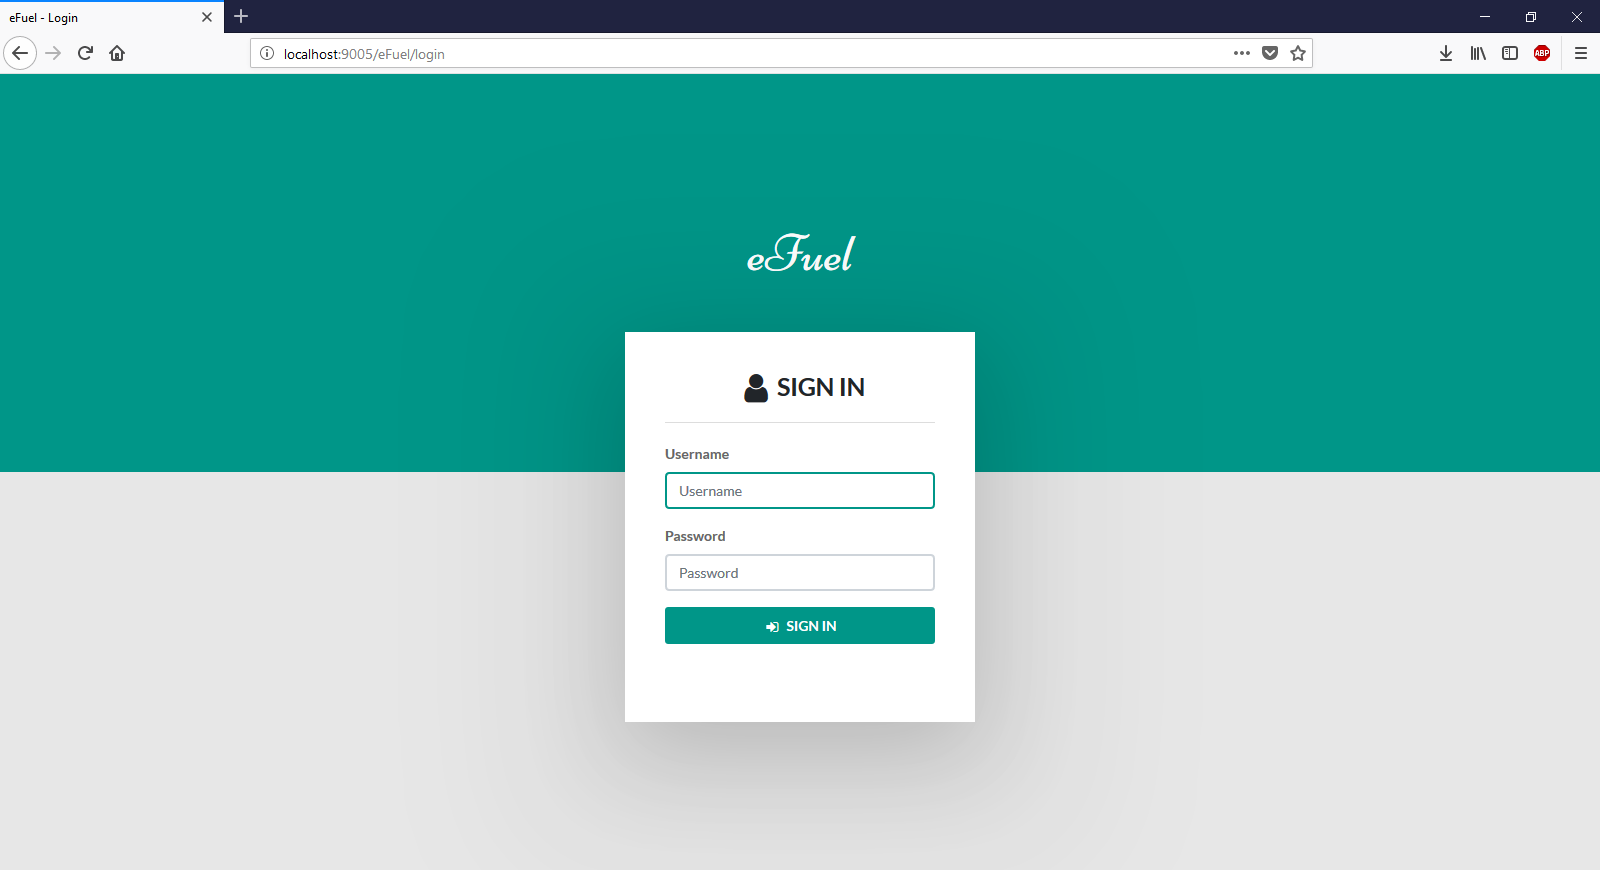
\includegraphics[width=\textwidth]{vistas/frontend/login.png}
    \caption{Inicio de Sesión}
    \label{fig:frontend:login}
    \centering
\end{figure}

\begin{figure}[H]
    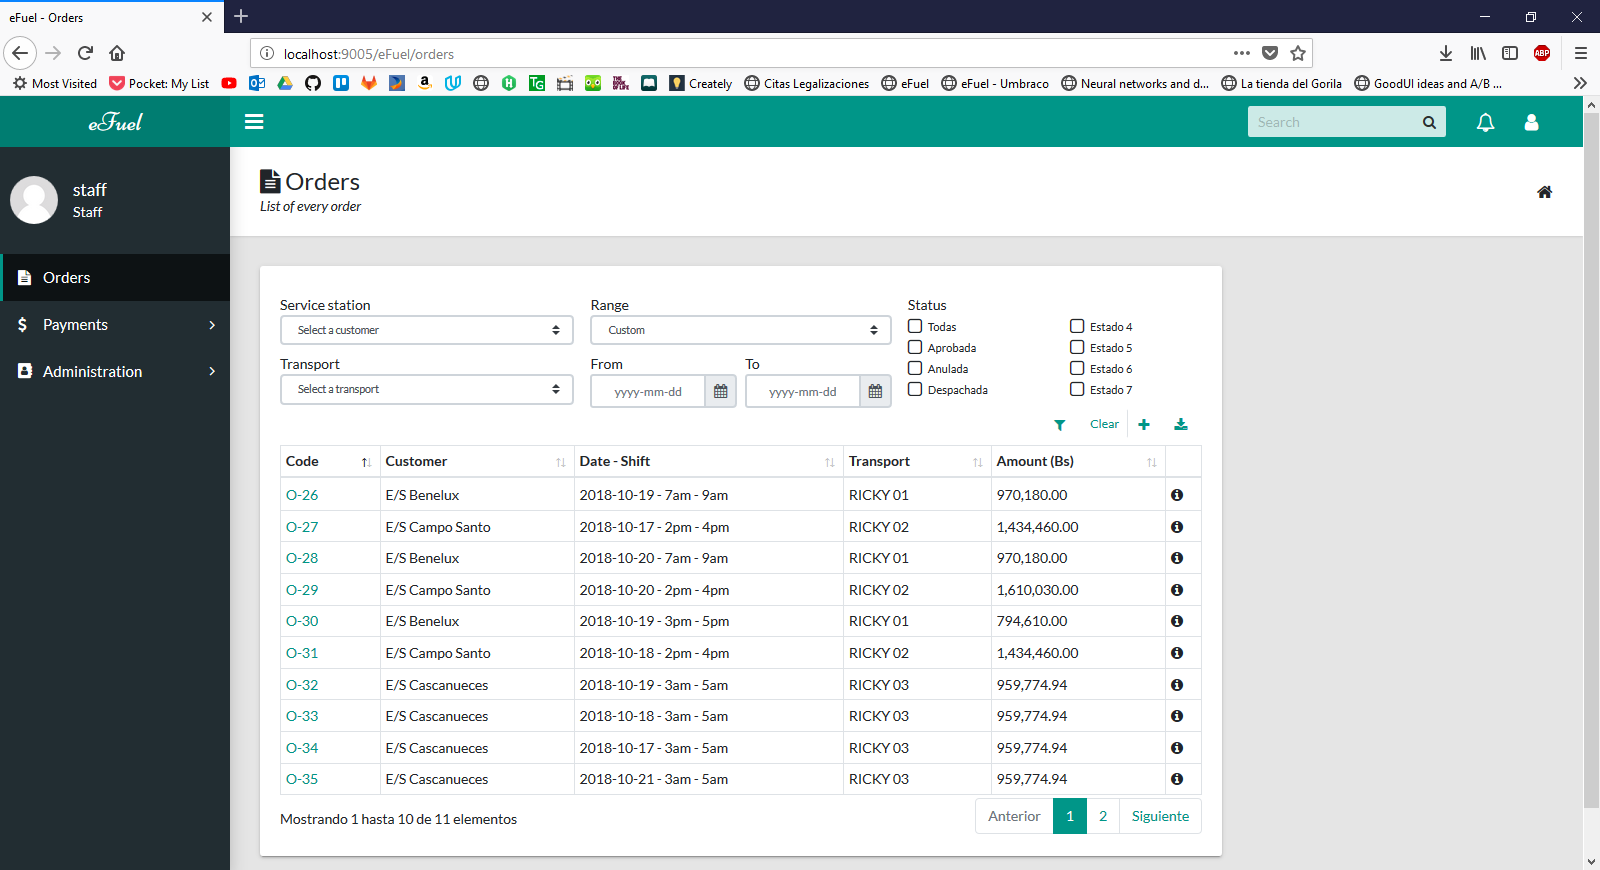
\includegraphics[width=\textwidth]{vistas/frontend/orders_list.png}
    \caption{Lista de pedidos}
    \label{fig:frontend:orders_list}
    \centering
\end{figure}

\begin{figure}[H]
    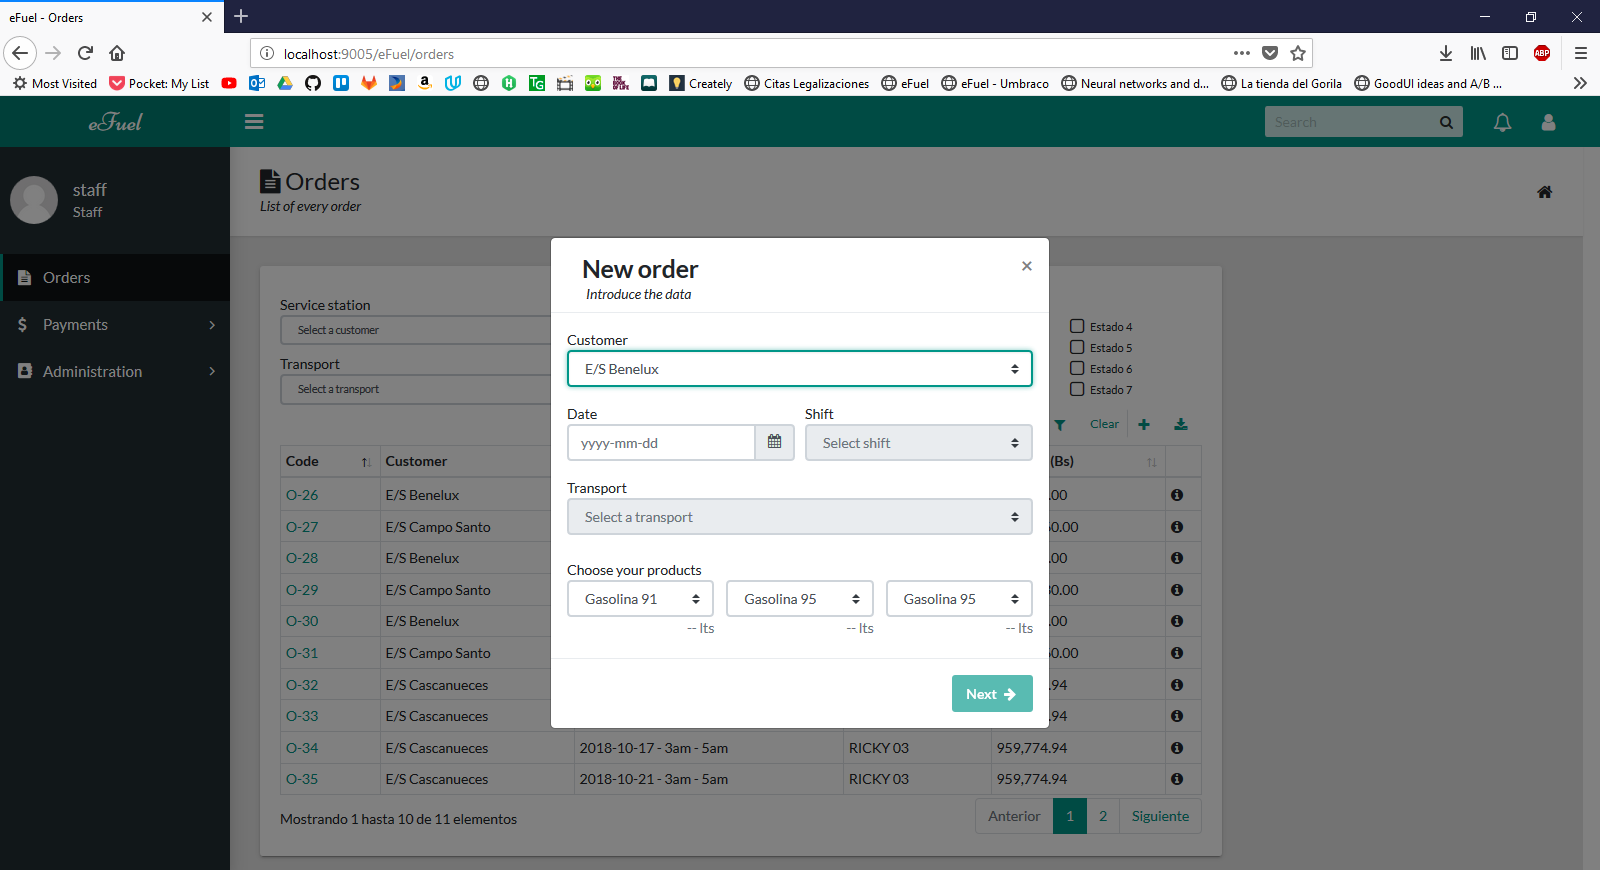
\includegraphics[width=\textwidth]{vistas/frontend/orders_create.png}
    \caption{Crear un pedido}
    \label{fig:frontend:orders_create}
    \centering
\end{figure}

\begin{figure}[H]
    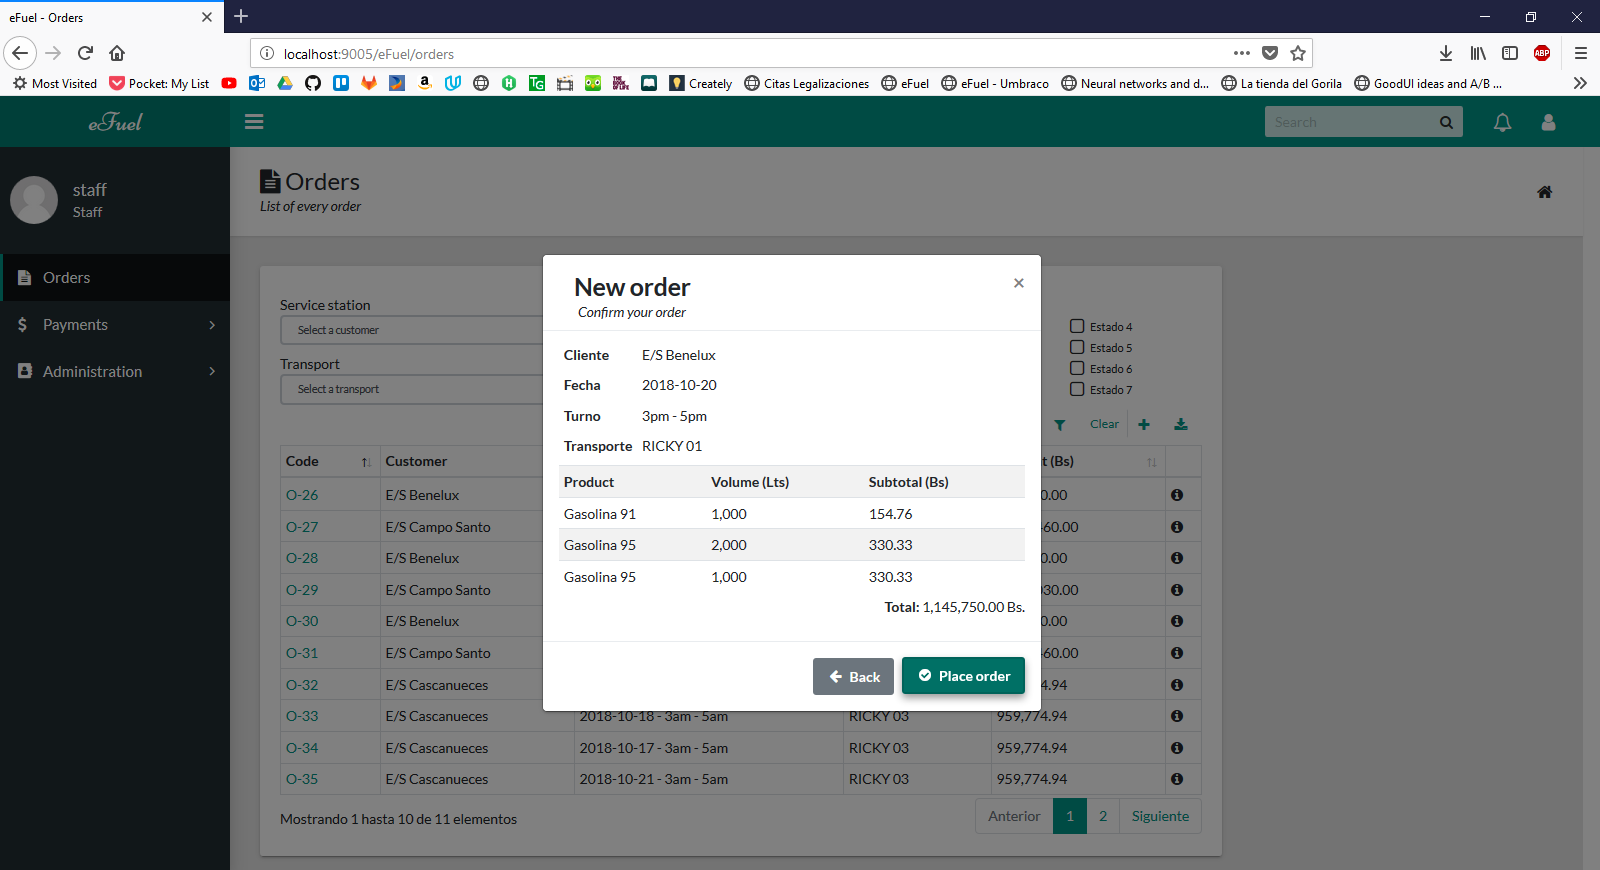
\includegraphics[width=\textwidth]{vistas/frontend/orders_create_preview.png}
    \caption{Crear un pedido - Preview}
    \label{fig:frontend:orders_create_preview}
    \centering
\end{figure}

\begin{figure}[H]
    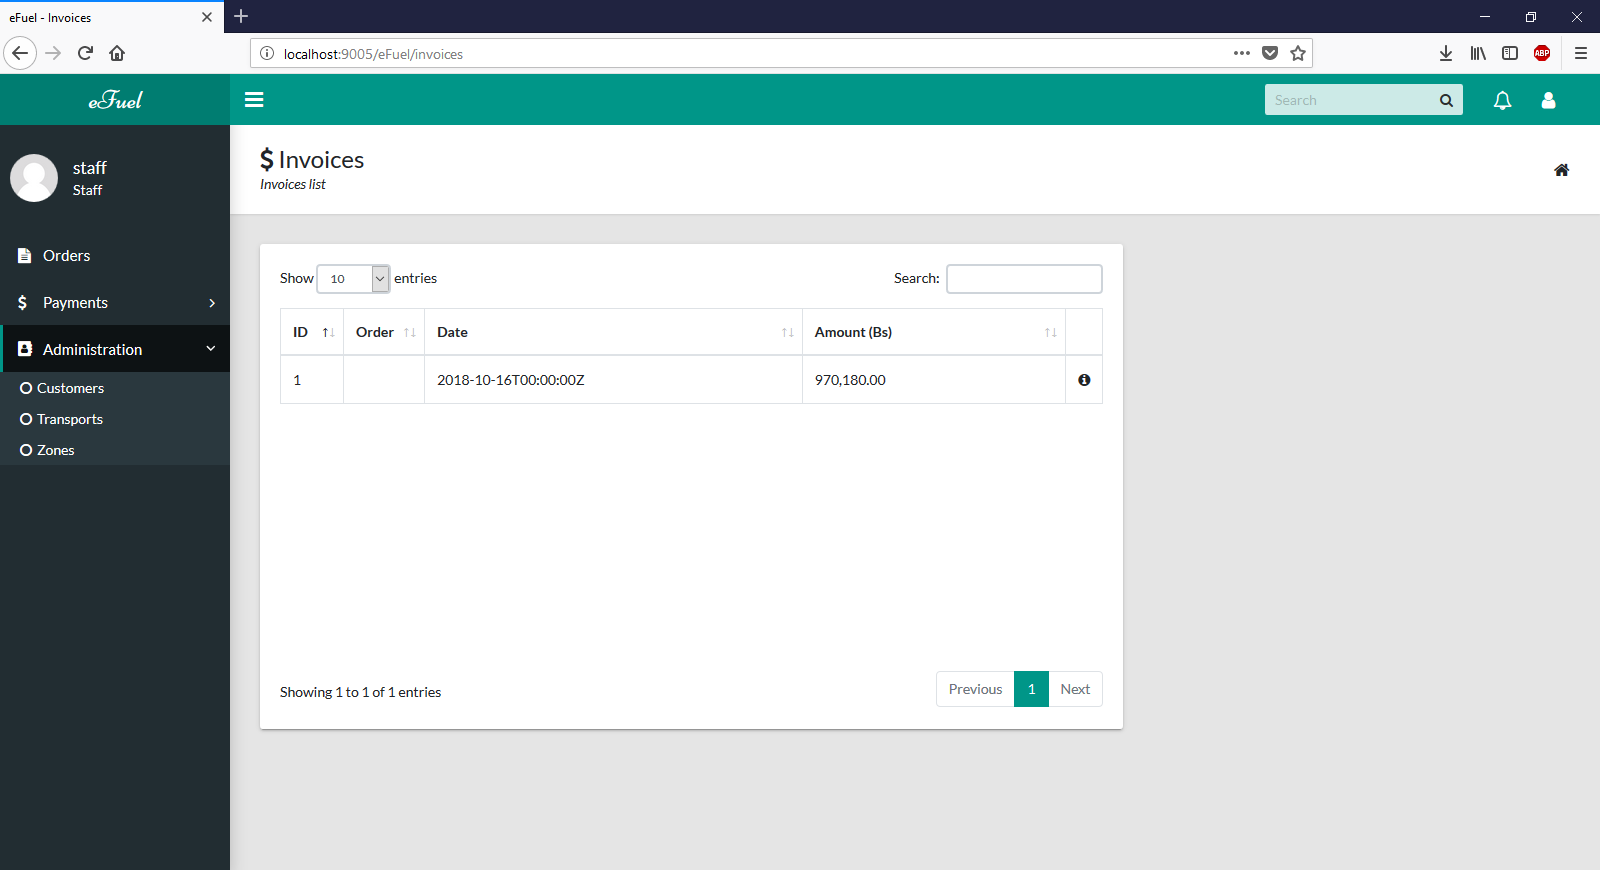
\includegraphics[width=\textwidth]{vistas/frontend/invoices_list.png}
    \caption{Lista de facturas}
    \label{fig:frontend:invoices_list}
    \centering
\end{figure}

\begin{figure}[H]
    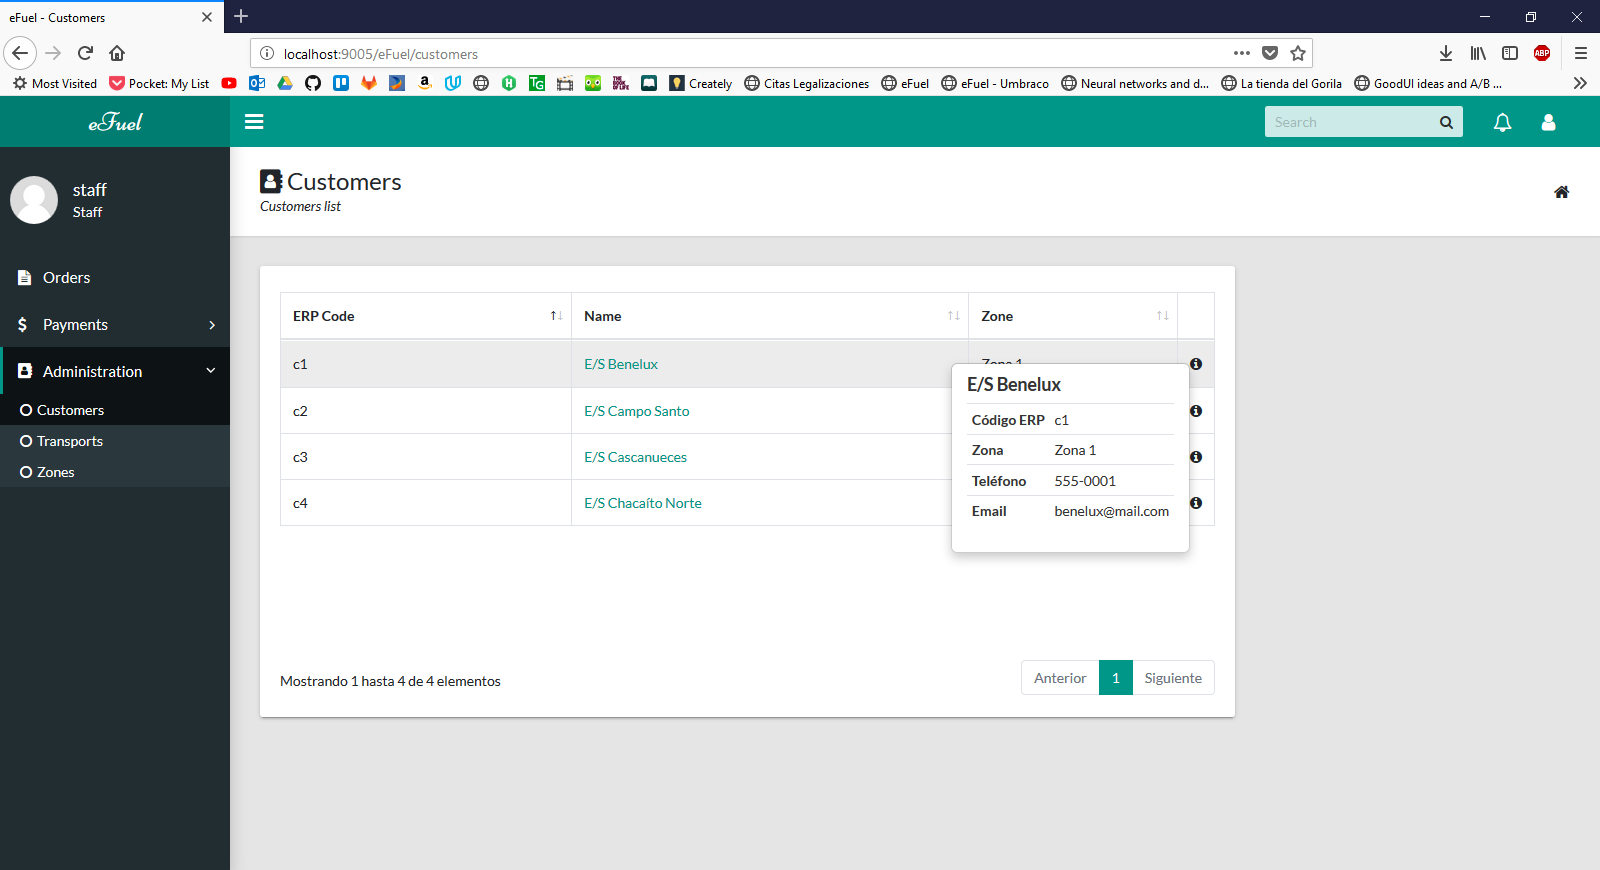
\includegraphics[width=\textwidth]{vistas/frontend/customers_list.png}
    \caption{Lista de clientes}
    \label{fig:frontend:customers_list}
    \centering
\end{figure}

\begin{figure}[H]
    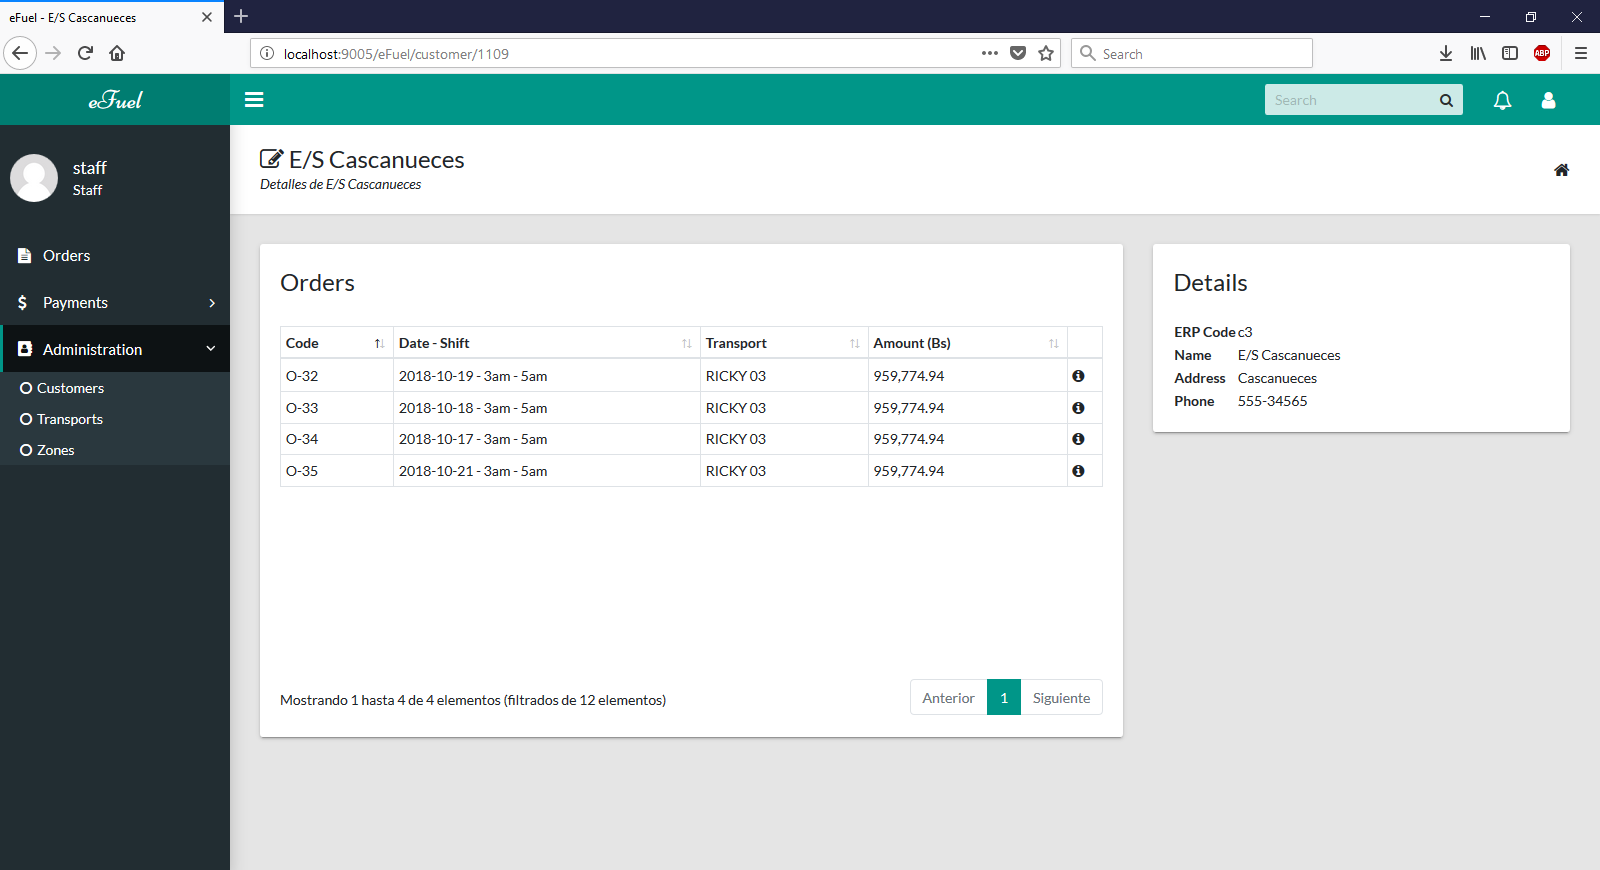
\includegraphics[width=\textwidth]{vistas/frontend/customers_detail.png}
    \caption{Detalles de cliente}
    \label{fig:frontend:customers_detail}
    \centering
\end{figure}

\begin{figure}[H]
    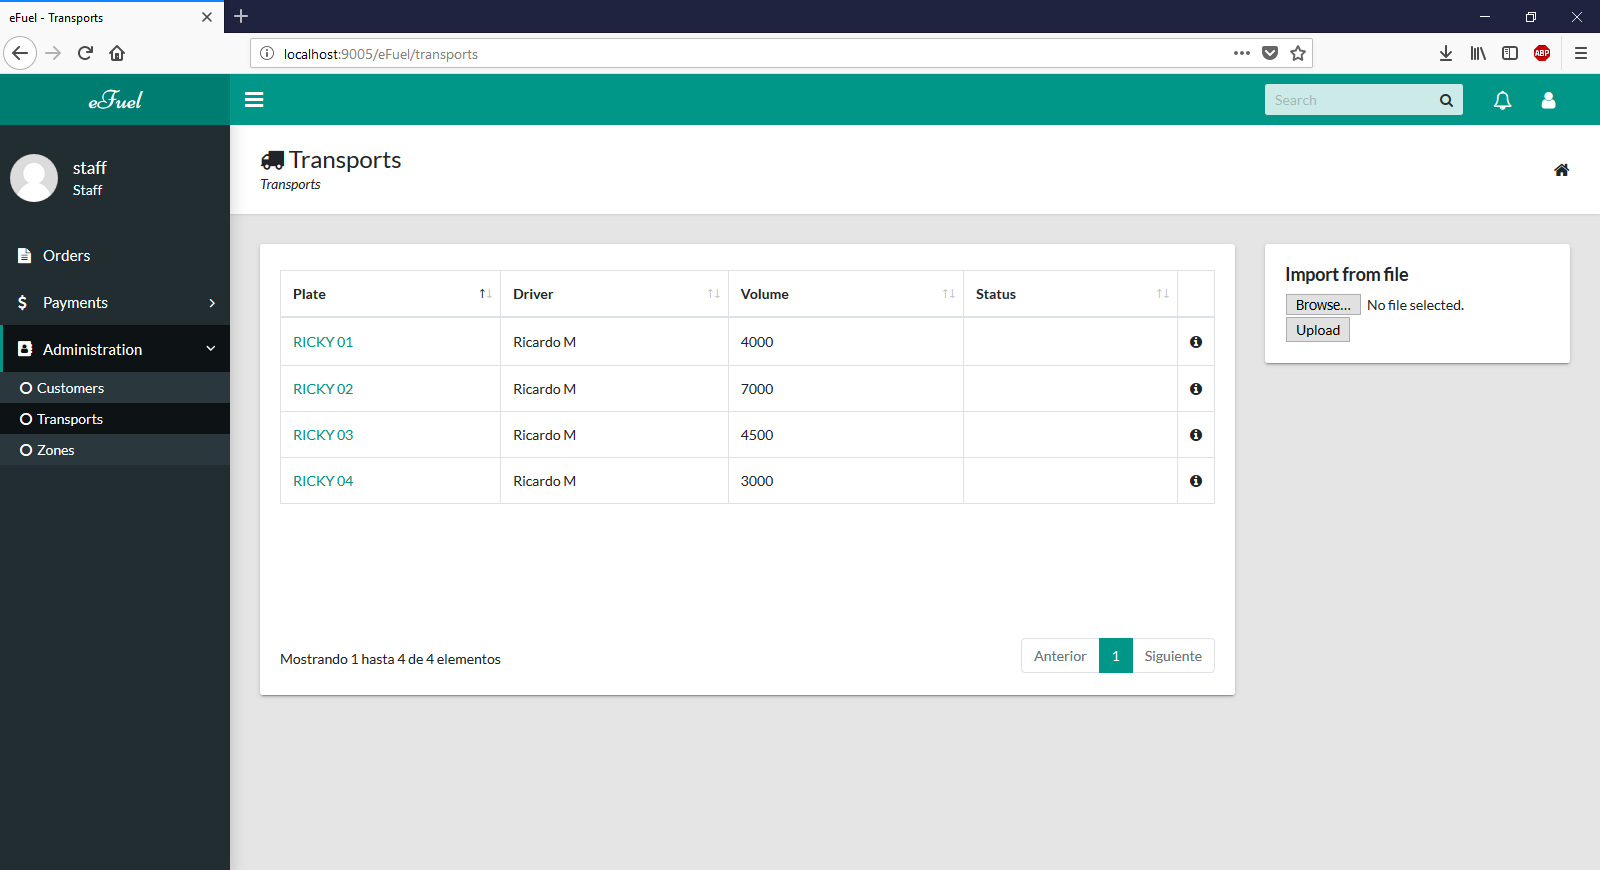
\includegraphics[width=\textwidth]{vistas/frontend/transports_list.png}
    \caption{Dashboard de transportes}
    \label{fig:frontend:transports_list}
    \centering
\end{figure}

\begin{figure}[H]
    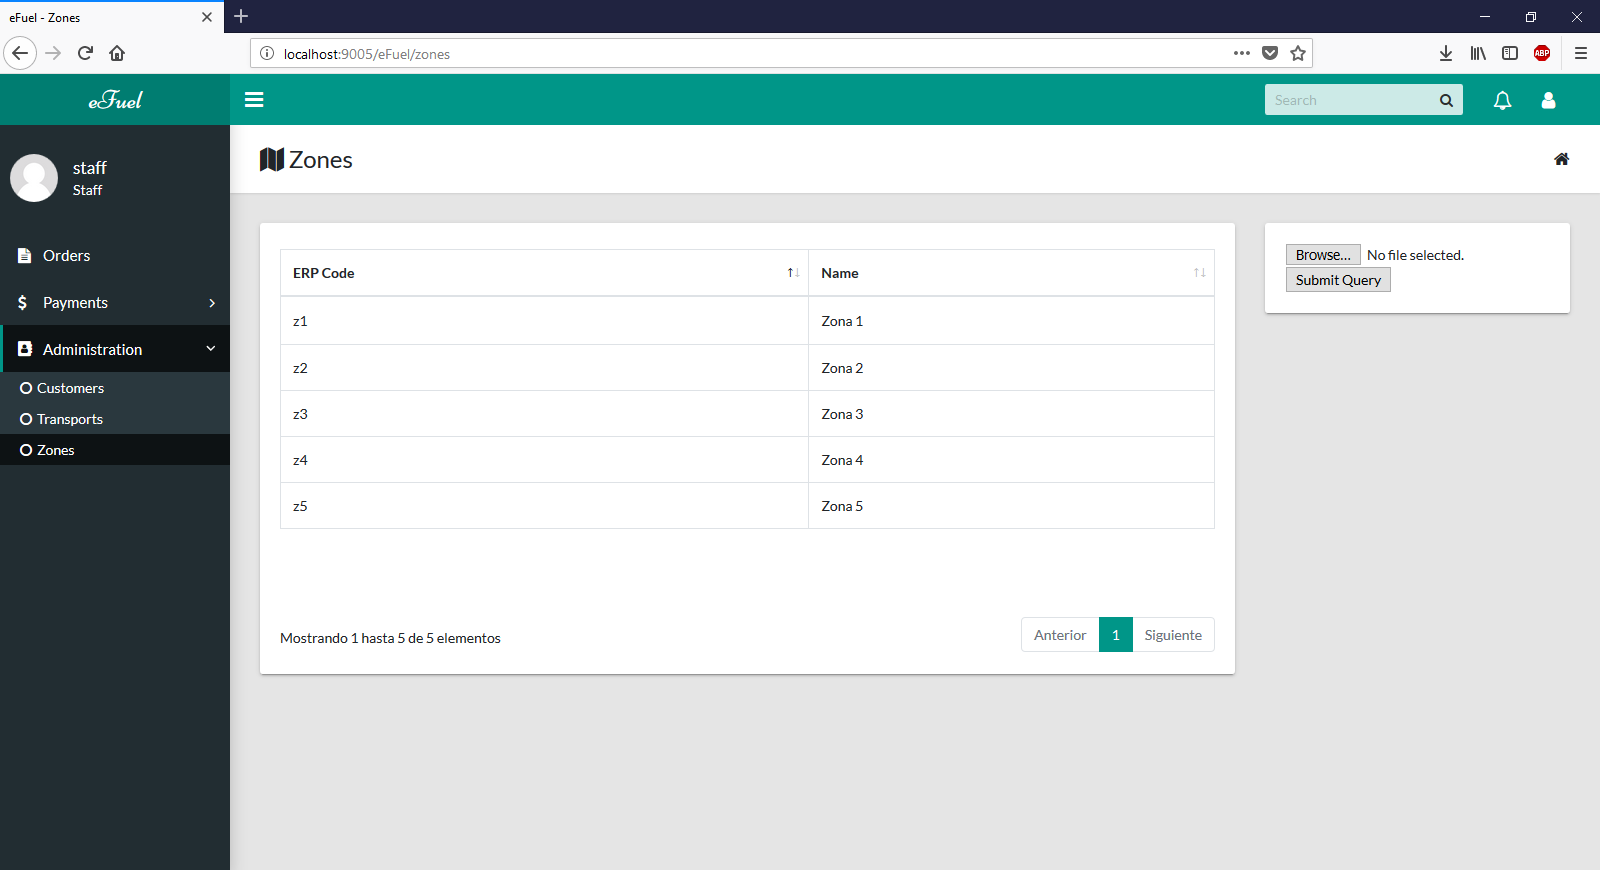
\includegraphics[width=\textwidth]{vistas/frontend/zones_list.png}
    \caption{Dashboard de zonas}
    \label{fig:frontend:zones_list}
    \centering
\end{figure}

\section{Back end (Umbraco)}
\begin{figure}[H]
    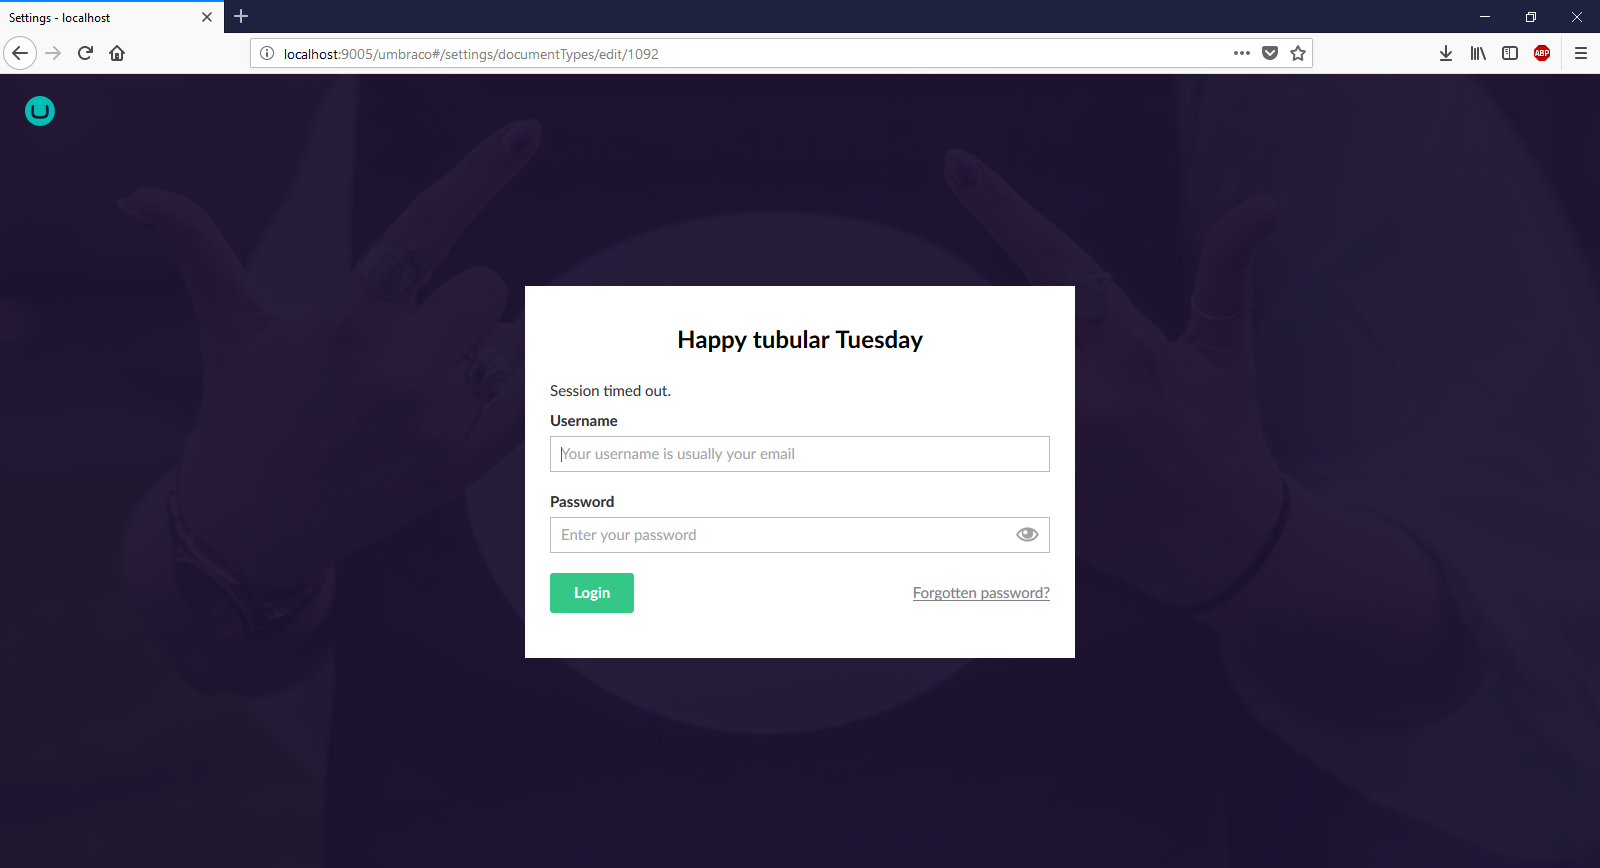
\includegraphics[width=\textwidth]{vistas/backend/login.png}
    \caption{Inicio de sesión (Umbraco)}
    \label{fig:backend:login}
    \centering
\end{figure}

\begin{figure}[H]
    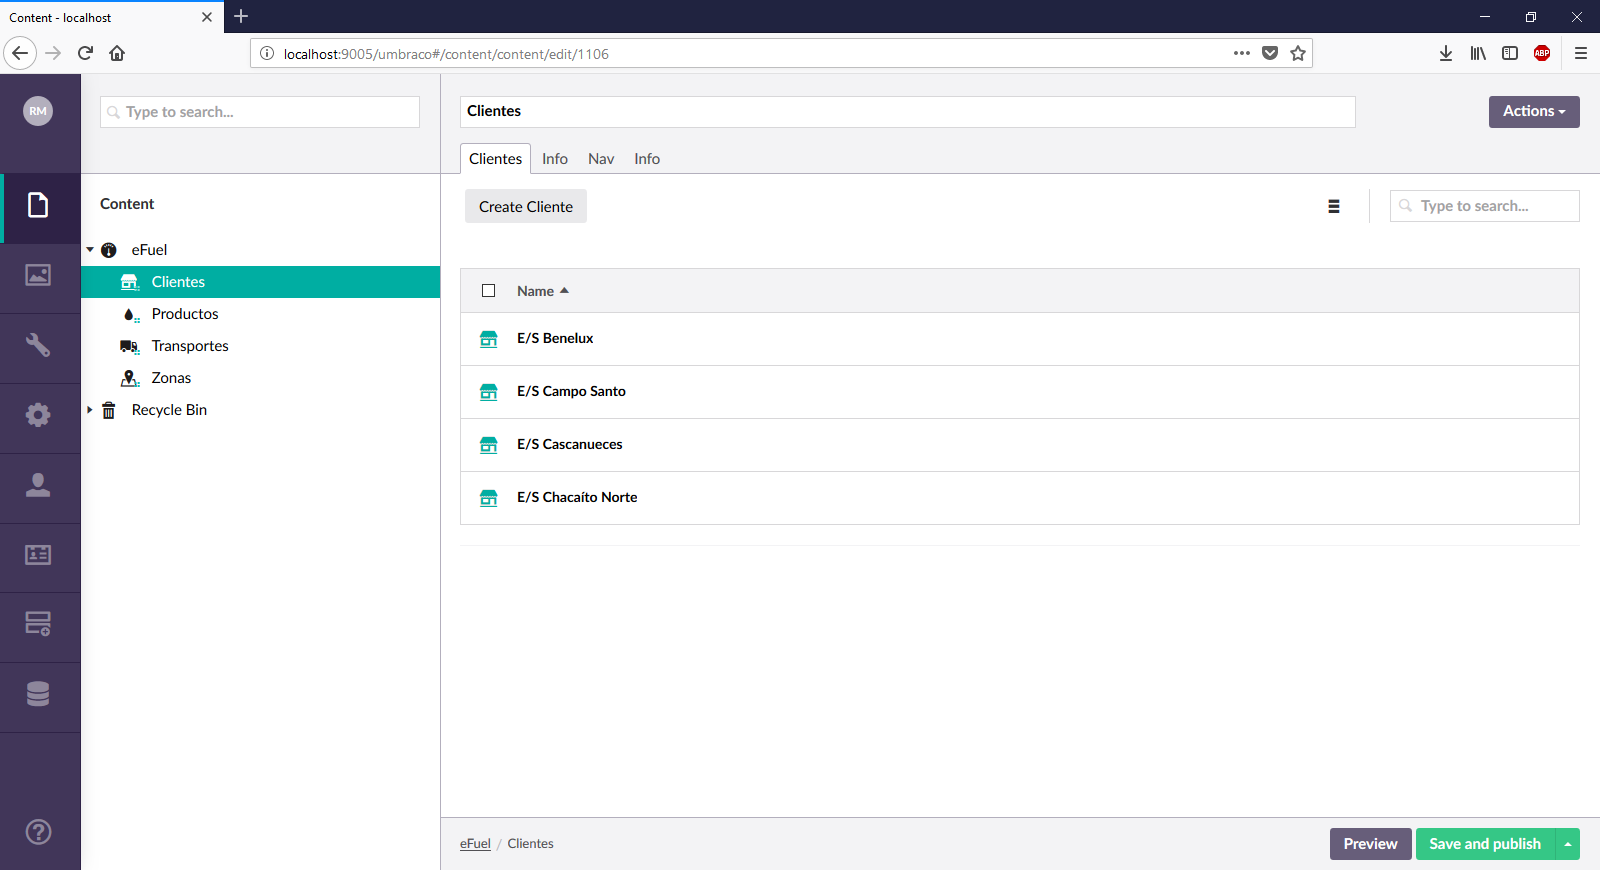
\includegraphics[width=\textwidth]{vistas/backend/list.png}
    \caption{Lista de clientes}
    \label{fig:backend:list}
    \centering
\end{figure}

\begin{figure}[H]
    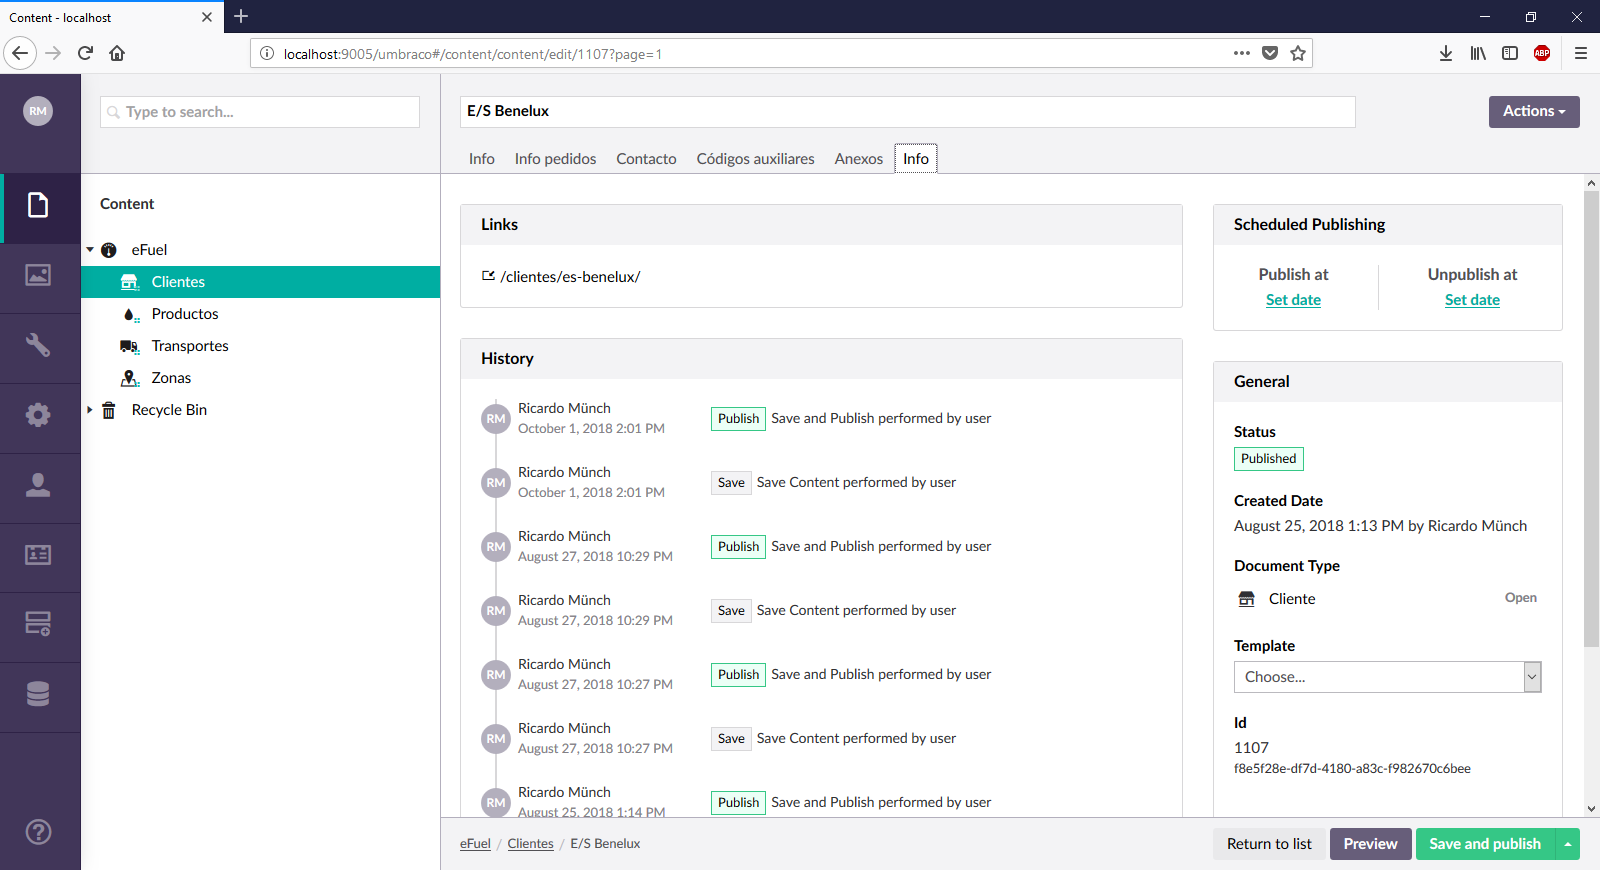
\includegraphics[width=\textwidth]{vistas/backend/details.png}
    \caption{Detalles de cliente}
    \label{fig:backend:details}
    \centering
\end{figure}

\begin{figure}[H]
    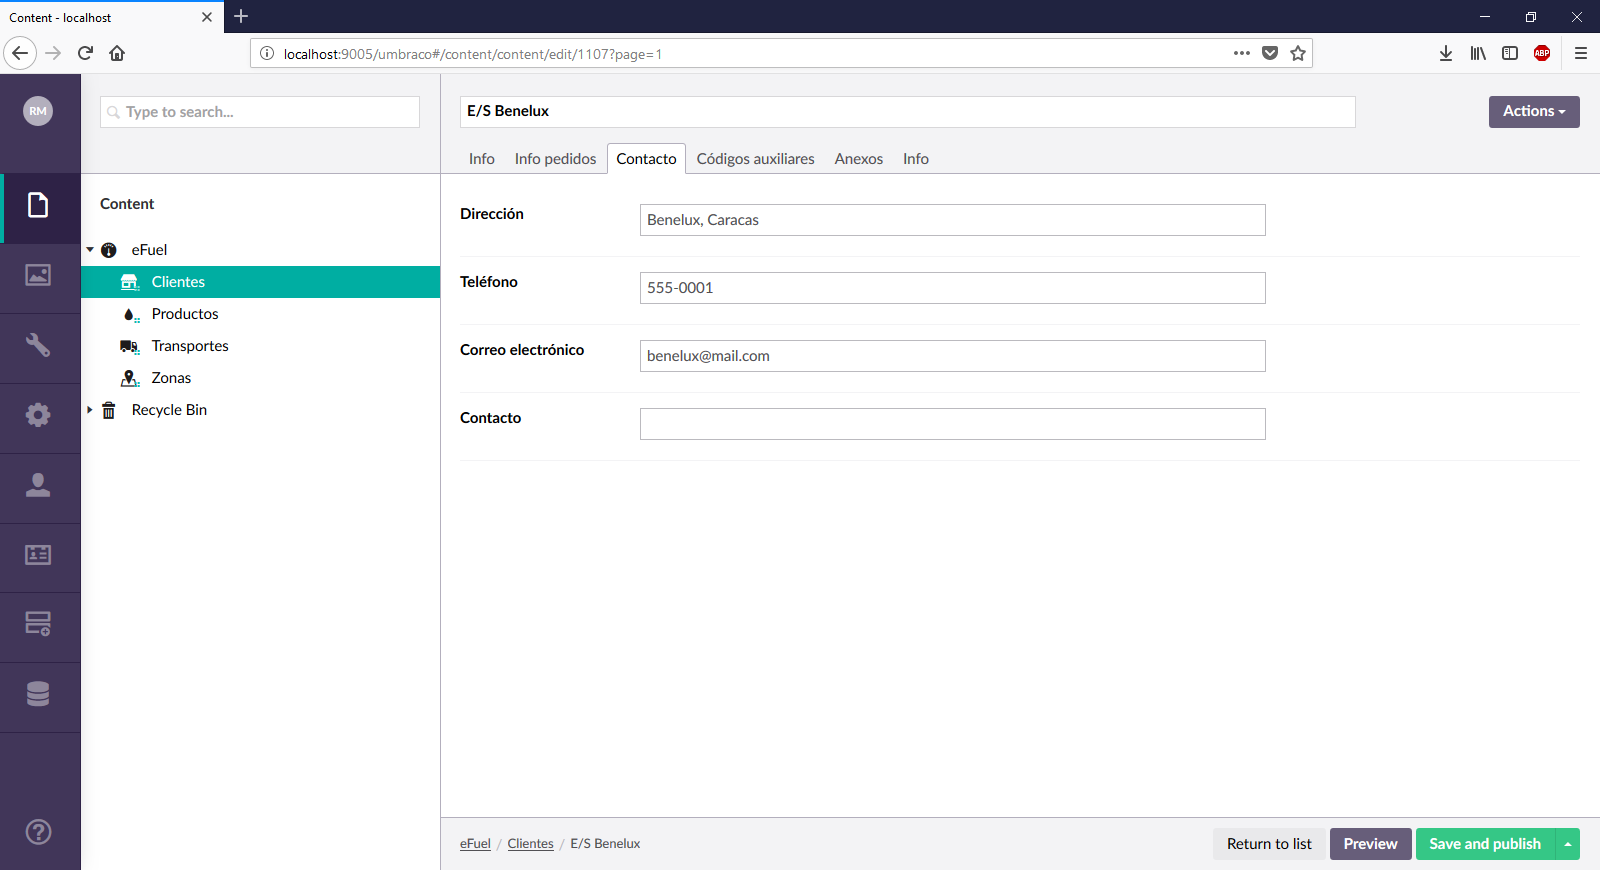
\includegraphics[width=\textwidth]{vistas/backend/edit.png}
    \caption{Editar cliente}
    \label{fig:backend:edit}
    \centering
\end{figure}

\begin{figure}[H]
    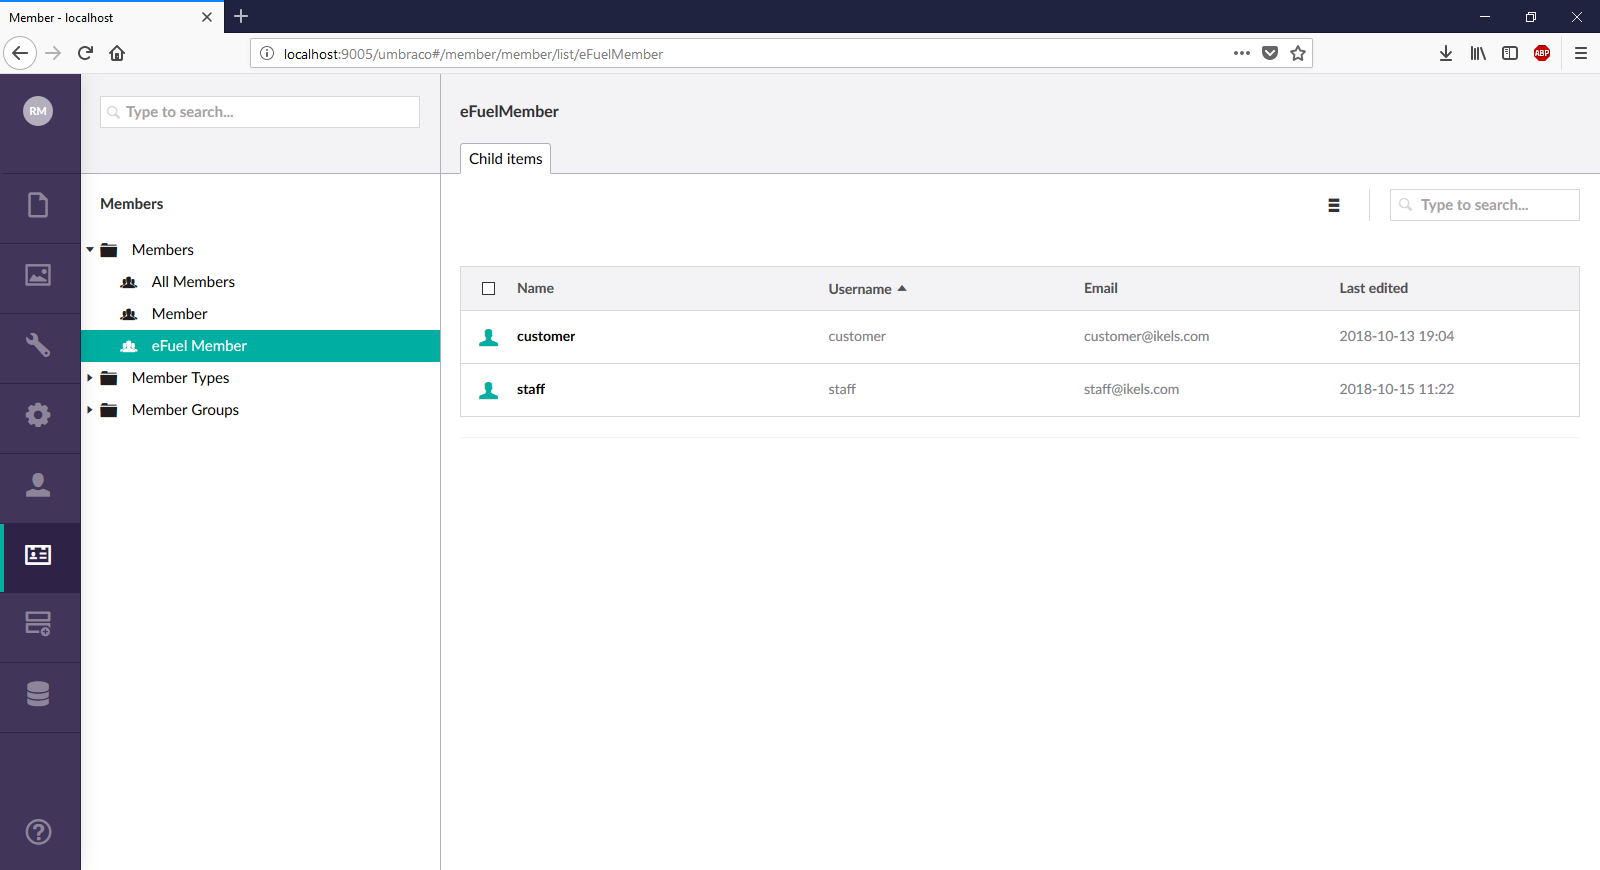
\includegraphics[width=\textwidth]{vistas/backend/members.png}
    \caption{Administración de miembros}
    \label{fig:backend:members}
    \centering
\end{figure}

\begin{figure}[H]
    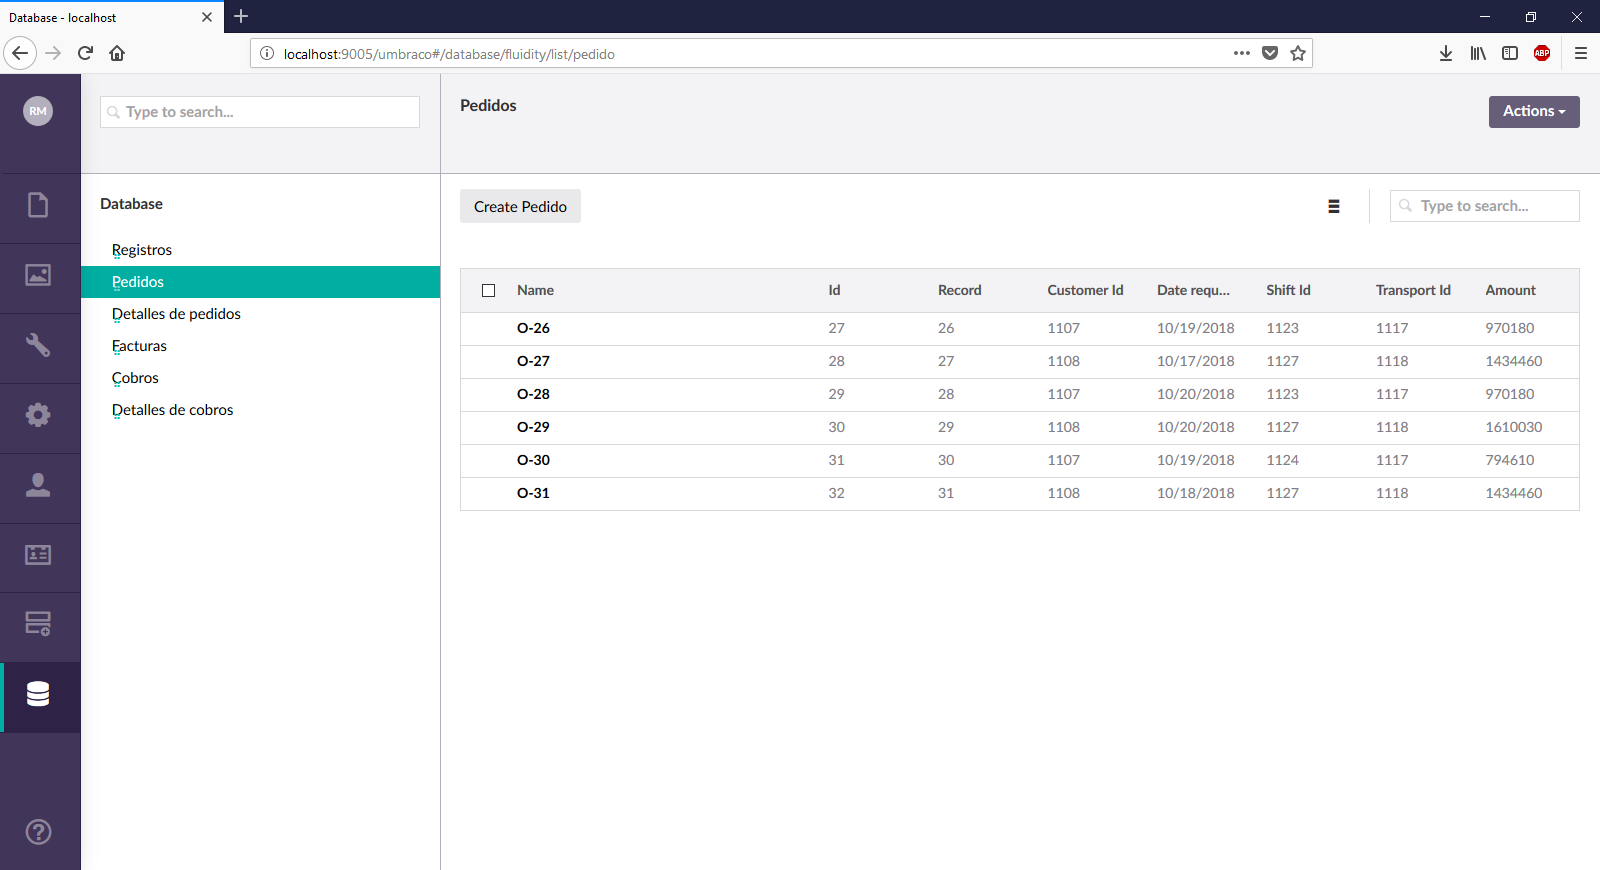
\includegraphics[width=\textwidth]{vistas/backend/flu_list.png}
    \caption{Lista de pedidos (Fluidity)}
    \label{fig:backend:flu_list}
    \centering
\end{figure}

\begin{figure}[H]
    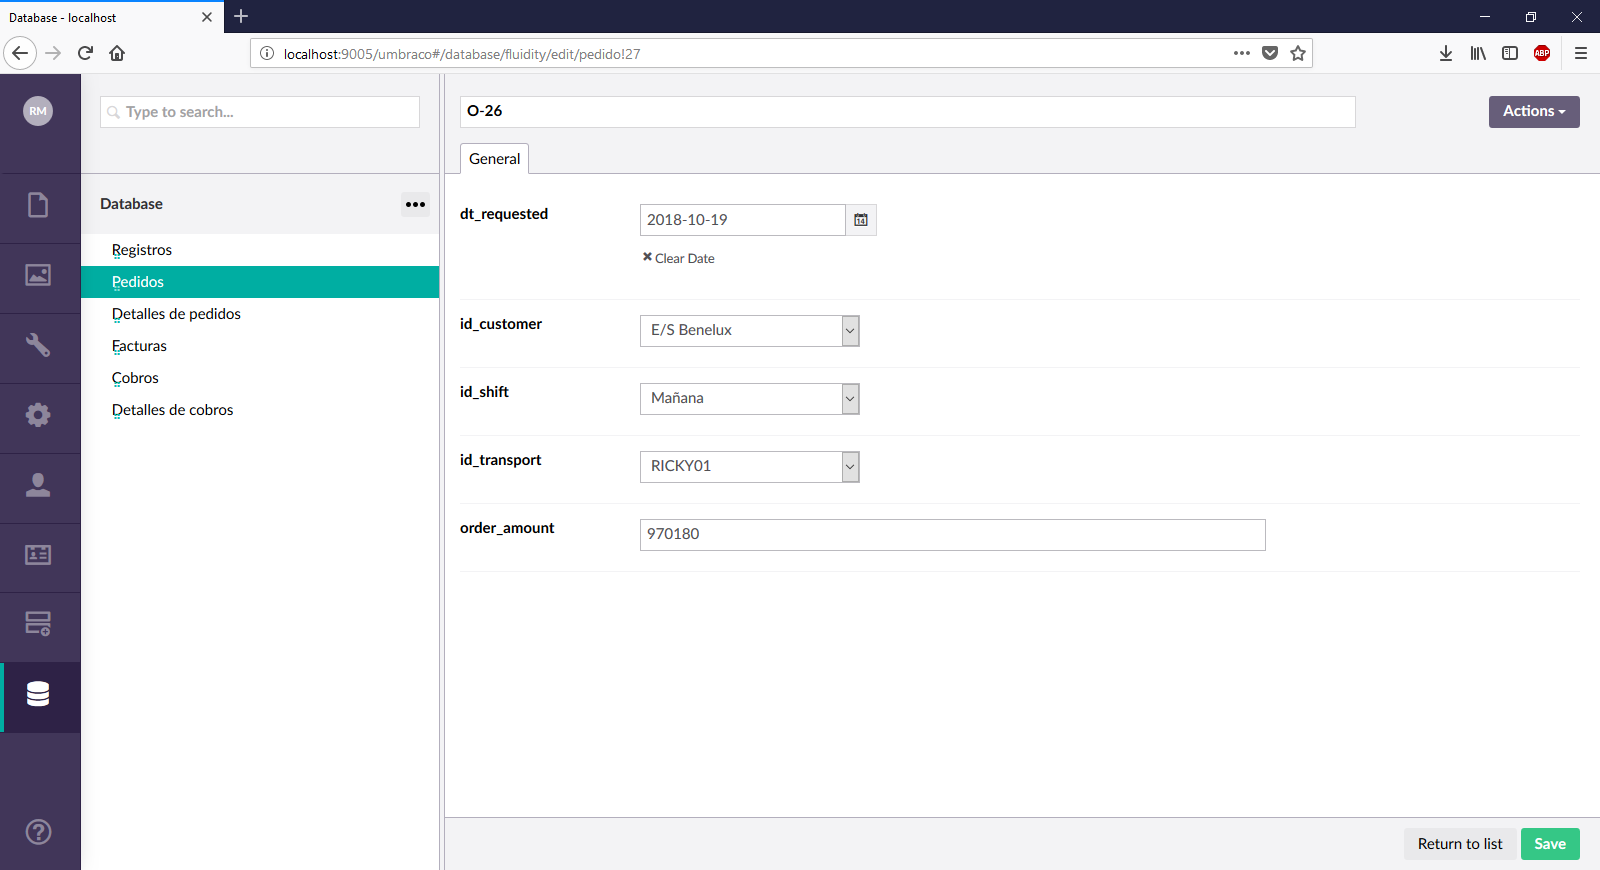
\includegraphics[width=\textwidth]{vistas/backend/flu_detail.png}
    \caption{Detalles de pedido (Fluidity)}
    \label{fig:backend:flu_detail}
    \centering
\end{figure}
    \chapter{GUÍA DE INSTALACIÓN EFUEL} \label{installation}

    \chapter{DOCUMENTO DE ARQUITECTURA DE SOFTWARE} \label{das}
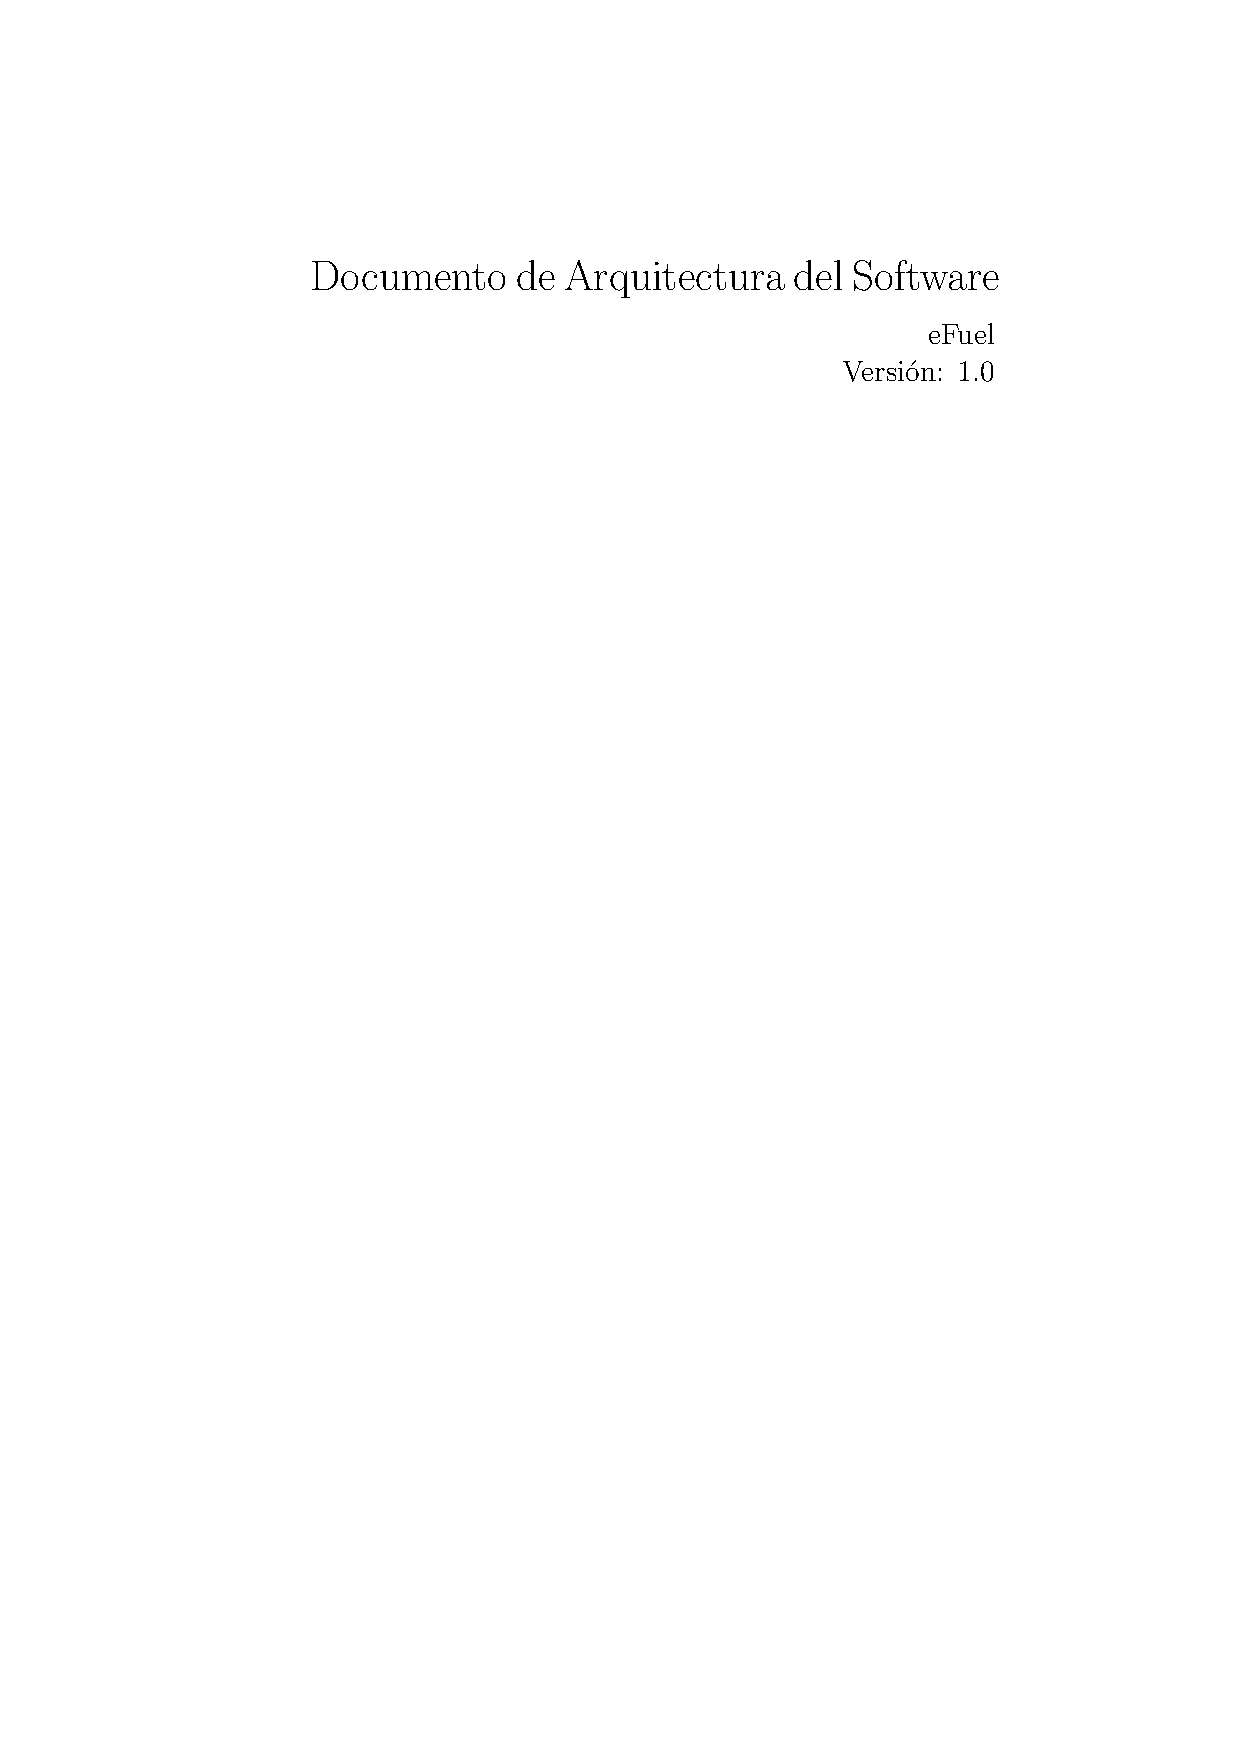
\includepdf[pages=-]{../anexos/das/das.pdf}

\end{document}
